% tirlnx01 - Materiaal om het keuzevak Linux te geven 
% op de Hogeschool Rotterdam.
% Copyright (C) 2010 - 2011  Paul Sohier, Kevin van der Vlist
%
% This program is free software: you can redistribute it and/or modify
% it under the terms of the GNU General Public License as published by
% the Free Software Foundation, either version 3 of the License, or
% (at your option) any later version.
%
% This program is distributed in the hope that it will be useful,
% but WITHOUT ANY WARRANTY; without even the implied warranty of
% MERCHANTABILITY or FITNESS FOR A PARTICULAR PURPOSE.  See the
% GNU General Public License for more details.
%
% You should have received a copy of the GNU General Public License
% along with this program.  If not, see <http://www.gnu.org/licenses/>.
%
% Kevin van der Vlist - kevin@kevinvandervlist.nl
% Paul Sohier - paul@paulsohier.nl

\documentclass[a4paper,11pt]{report}
% Hier hebben we de preamble, alle document settings moeten hier:
\usepackage{graphicx}
\usepackage{url}
\usepackage{appendix}
\usepackage[titles]{tocloft}
\usepackage[dutch]{babel}
\usepackage{listings}
\usepackage{makeidx}
\usepackage{float}
\usepackage[hypertexnames=false]{hyperref}
\usepackage{fancyhdr}
\usepackage{tipa}

% Custom LaTeX commands:
% ~ == {\raise.17ex\hbox{$\scriptstyle\sim$}}
\newcommand{\customtilde}{\raise.17ex\hbox{$\scriptstyle\sim$}}
% Meta info pdf:
\hypersetup{
%bookmarks=true, % show bookmarks bar?
unicode=false, % non-Latin characters in Acrobat’s bookmarks
pdftoolbar=true, % show Acrobat’s toolbar?
pdfmenubar=false, % show Acrobat’s menu?
pdffitwindow=false, % window fit to page when opened
%pdfstartview={FitH}, % fits the width of the page to the window
pdftitle={TIRLNX01}, % title
pdfauthor={Paul Sohier, Kevin van der Vlist}, % author
pdfsubject={Inleiding Linux}, % subject of the document
pdfcreator={make}, % creator of the document
pdfproducer={make}, % producer of the document
pdfkeywords={Linux} {Basis}, % list of keywords
pdfnewwindow=true, % links in new window
colorlinks=false, % false: boxed links; true: colored links
linkcolor=black, % color of internal links
citecolor=green, % color of links to bibliography
filecolor=magenta, % color of file links
urlcolor=cyan % color of external links
}

% Paragrafen hebben een witregel ertussen, en geen indent tab:
\setlength{\parindent}{0.0in}
\setlength{\parskip}{0.1in}
% Onderstaande is voor de dots tussen chapter title + blz. 
\makeatletter
\renewcommand*\l@chapter[2]{%
  \ifnum \c@tocdepth >\m@ne
    \addpenalty{-\@highpenalty}%
    \vskip 1.0em \@plus\p@
    \setlength\@tempdima{1.5em}%
    \begingroup
      \parindent \z@ \rightskip \@pnumwidth
      \parfillskip -\@pnumwidth
      \leavevmode \bfseries
      \advance\leftskip\@tempdima
      \hskip -\leftskip
      #1\nobreak\normalfont\leaders\hbox{$\m@th
        \mkern \@dotsep mu\hbox{.}\mkern \@dotsep
        mu$}\hfill\nobreak\hb@xt@\@pnumwidth{\hss #2}\par
      \penalty\@highpenalty
    \endgroup
  \fi}
\makeatother

% End of title + blz.
% Table of content depth van 4, dus tm paragraph
\setcounter{tocdepth}{4}
%\renewcommand{\baselinestretch}{1.5} 1.5 regelafstand 

%Pas listings aan zodat ze duidelijker zijn
\lstset{ %
  language=bash,                % choose the language of the code
  basicstyle=\footnotesize,       % the size of the fonts that are used for the code
  numbers=left,                   % where to put the line-numbers
  numberstyle=\footnotesize,      % the size of the fonts that are used for the line-numbers
  numbersep=5pt,                  % how far the line-numbers are from the code
  showspaces=false,               % show spaces adding particular underscores
  showstringspaces=false,         % underline spaces within strings
  showtabs=false,                 % show tabs within strings adding particular underscores
  frame=lr,	                % adds left and right lines
  tabsize=2,	                % sets default tabsize to 2 spaces
  captionpos=b,                   % sets the caption-position to bottom
  breaklines=true,                % sets automatic line breaking
  breakatwhitespace=false,        % sets if automatic breaks should only happen at whitespace
%  escapeinside={\%*}{*)},         % if you want to add a comment within your code
  morekeywords={*,...}            % if you want to add more keywords to the set
}
%hyperref aanpassingen
\hypersetup{pdfborder=0 0 0}

% We gebruiken de index
\makeindex

% Footer
% \runningfooter{Paul Sohier\\Kevin van der Vlist}{TIRLNX01\\Hogeschool Rotterdam}{\thepage}
\pagestyle{fancy}

\renewcommand{\headrulewidth}{0.0pt}

\lhead{}
\chead{}
\rhead{}

\lfoot{Paul Sohier\\Kevin van der Vlist}
\cfoot{TIRLNX01\\Hogeschool Rotterdam}
\rfoot{Pagina\\\thepage}

% Ook in chapters
\fancypagestyle{plain}{\pagestyle{fancy}}

% Einde preamble, begin document; 
\begin{document}
% Title page
\begin{titlepage}
\vspace*{\fill}
\begin{center}

\textsc{\Huge \bfseries TIRLNX01}\\[0.5cm]
{\large \bfseries Keuzevak Linux}\\[0.25cm]
{\large \bfseries Dictaat}\\[1.5cm]

\begin{minipage}{0.4\textwidth}
\begin{flushleft} \large
\texttt{Auteurs:}\\
\ \\
\textsc{Kevin van der Vlist}\\
\href{mailto:kevin@kevinvandervlist.nl}{kevin@kevinvandervlist.nl}\\
\ \\
\texttt{en}\\
\ \\
\textsc{Paul Sohier}\\
\href{mailto:paul@paulsohier.nl}{paul@paulsohier.nl}
\end{flushleft}
\end{minipage}
\begin{minipage}{0.5\textwidth}

\begin{flushright} \large
\texttt{Gedoceerd te:}\\
\ \\
\textsc{Hogeschool Rotterdam}\\
Vestiging Academieplein
\end{flushright}
\end{minipage}
{\ }\\[1.5cm]
{\large Versie 1.2}\\[0.75cm]
{\large \today}
\vfill
\end{center}
\vspace*{\fill}
\end{titlepage}

% Abstract (+ in toc)?:
\begin{abstract}\centering
We proberen jullie wegwijs te maken binnen een Linux omgeving.\\
Hopelijk slagen we hierin.

\textsc{``Unix is user-friendly. It's just very selective about who its friends are.''}
\end{abstract}

% We baseren structuur op het dictaat Remko & Peter; vermelden
\phantomsection
\addcontentsline{toc}{chapter}{\numberline{}Voorwoord}
\chapter*{Voorwoord}
De structuur van dit dictaat is gebaseerd op het dictaat \textsl{Linux Starter Pack}\cite{bib.rvrijpb}, geschreven door Remko de Vrijer en Peter Berends. We hebben de structuur als basis gebruikt, en verder het document helemaal herschreven met up to date informatie. Daarnaast is het document ook uitgebreid met extra informatie. Enkele kleine delen van de tekst, voornamelijk van technieken die momenteel weinig gebruikt worden, zullen nog uit het originele document komen. 

% De table of contents + toc in toc:
\tableofcontents
\addcontentsline{toc}{chapter}{\numberline{}Inhoudsopgave}

% Inleiding:
\chapter*{Inleiding}
\addcontentsline{toc}{chapter}{\numberline{}Inleiding}
Dit dictaat is erop gericht om jullie op een goede manier in te leiden binnen een \emph{GNU/Linux} systeem. We zullen dit echter op een andere manier aanpakken dan men in eerste instantie zou denken. 

Om een duidelijk beeld te cre\"{e}eren zonder verschillende termen door elkaar te halen zullen door het dictaat de volgende drukstijlen gebruikt worden. 
\begin{itemize}
\item[1.] Normale tekst is gewoon uitleg.
\item[2.] ``Tekst in quotes'' zal betekenen dat we dingen extra willen benadrukken. Denk aan gebruikersnamen en menu-items. 
\item[3.] \emph{Schuin gedrukte woorden} zullen begrippen of namen zijn.
% Alle commando's in de \index{} voor reference. 
\item[4.] Commando's zullen in \texttt{monospaced font} afgedrukt zijn. 
\item[5.] Voorbeelden met code of de uitvoer van commando's zullen in blokken verschijnen met regelnummers. Regelnummers zijn geen onderdeel van de code.
\begin{lstlisting}
Dit is een voorbeeld.
\end{lstlisting}
\end{itemize}
Als eerste zal er duidelijk gemaakt moeten worden dat er niet op een ``grafische'' manier naar een systeem gekeken zal worden. Er zal namelijk geen gebruik gemaakt worden van een \emph{GUI}. De reden hiervoor is de drang om een systeem ``te verbergen'' voor gebruikers. Deze krijgen hierdoor geen mogelijkheid om eens goed onder de motorkap te kijken. 

Ook zal er in server situaties geen \emph{GUI} gebruikt worden. Waarom zou iemand de kostbare resources van een server willen verspillen aan rekentijd voor een grafische omgeving? Dit geldt alleen maar sterker als de snelheid van een geoefende \emph{shell} gebruiker in ogenschouw wordt genomen. 

Dit dictaat zal worden gericht op de distributie \emph{Slackware}. Hier is voor gekozen omdat het relatief weinig wordt gebruikt en omdat het een puristische instelling heeft met betrekking tot de inrichting van het systeem. Dit resulteert in meer ``handwerk'' om het systeem te configureren, maar laat wel beter zien hoe het nu precies in elkaar zit. 

We hopen dat dit dictaat jullie zal helpen bij het begrijpen van de \emph{GNU/Linux} wereld.
% Einde inleiding

% HACK: Page number fixen. Dit is voor makeidx + hyperref
% 13 is de pagina met hoofdstuk 01, dus inleiding erop. 
% Dit zorgt ervoor dat alle
\setcounter{page}{13}
% Nu kunnen we de losse hoofdstukken gaan includen. 
% Includen gebeurt met basename, dus zonder .tex
% tirlnx01 - Materiaal om het keuzevak Linux te geven 
% op de Hogeschool Rotterdam.
% Copyright (C) 2010 - 2011  Paul Sohier, Kevin van der Vlist
%
% This program is free software: you can redistribute it and/or modify
% it under the terms of the GNU General Public License as published by
% the Free Software Foundation, either version 3 of the License, or
% (at your option) any later version.
%
% This program is distributed in the hope that it will be useful,
% but WITHOUT ANY WARRANTY; without even the implied warranty of
% MERCHANTABILITY or FITNESS FOR A PARTICULAR PURPOSE.  See the
% GNU General Public License for more details.
%
% You should have received a copy of the GNU General Public License
% along with this program.  If not, see <http://www.gnu.org/licenses/>.
%
% Kevin van der Vlist - kevin@kevinvandervlist.nl
% Paul Sohier - paul@paulsohier.nl

\chapter{Introductie}
\emph{Linux} is net als \emph{Windows} een operating system, het ``programma'' wat draait op de computer en waarmee de computer bestuurd wordt. \emph{Linux} is ooit bedoeld geweest voor gebruik op een server en wordt daar ook op dit moment nog primair voor gebruikt. Ook als vervanger voor \emph{Windows}, met een grafische schil is \emph{Linux} tegenwoordig goed geschikt. Wel is er nog duidelijk te zien dat \emph{Linux} primair bedoeld is voor gebruik op  een server. Niet voor niets draait \emph{Linux} op de meeste web servers. De \emph{GUI} van \emph{Linux} is ook tegenwoordig goed bruikbaar voor normaal gebruik en er zijn dus ook steeds meer mensen die \emph{Linux} gebruiken voor hun ``normale'' computer. In dit dictaat gaan we geen gebruik maken van een \emph{GUI}\index{GUI}, maar gaan we  puur de \emph{Shell} gebruiken. Met een \emph{GUI} kan je vrij eenvoudig alles instellen en wijzigen, terwijl je met alleen een \emph{shell} je veel meer zelf moet doen.

\section{De geschiedenis}
In 1991 wilde de Finse student Linus Torvalds gebruik maken van \emph{UNIX}\index{UNIX}. Omdat \emph{UNIX} echter een betaald operating system was, ging hij aan de slag met \emph{Minix}. Dit voldeed al snel niet meer aan de eisen welke hij stelde en hij besloot een eigen kernel te gaan schrijven. Eigenlijk wilde hij een compleet operating system gaan maken, maar hij schreef uiteindelijk alleen de kernel. Naast de zelf geschreven kernel gebruikte hij de \emph{GNU tools}. Vandaar dat wanneer er tegenwoordig \emph{Linux} word gezegd, er de \emph{GNU/Linux} combinatie bedoeld wordt. \emph{Linux} is de kernel, met daarop de \emph{GNU tools} in \emph{userland}.\index{GNU}

De eerste versie was niet echt bruikbaar voor de gemiddelde mens, het was het meer een speeltje voor programmeurs en hackers. Door het open karakter en de actieve gebruikers gemeenschap is hier toch een stabiel en volledig werkend operating system uit voortgekomen. In 1994 kwam de eerste versie dan echt uit en sindsdien is de kernel ook sterk verbeterd. Tegenwoordig draait \emph{Linux} niet alleen op standaard computers, maar ook op \emph{embedded systemen}, zoals routers en \emph{telefoons}. In de toekomst zal dit alleen maar toenemen. Er zijn momenteel zelfs al koelkasten in de handel die een \emph{Linux} versie draaien.

De kernel is uiteraard ook op dit moment nog steeds in ontwikkeling. Onder leiding van Linus Torvalds worden er nog steeds nieuwe technieken ge\"{i}mplementeerd en fouten verbeterd. Uiteraard doet hij dit niet in zijn \'{e}\'{e}ntje, iedereen die wilt kan zijn bijdrage doen via de git repository van de kernel. Het aantal personen dat heeft gewerkt aan de source code van de \emph{Linux} kernel bedraagt vele duizenden.

\section{De GNU}
De \emph{GNU foundation} is opgericht door Richard Stallman. Hij is het project begonnen om een vrije implementatie van een \emph{UNIX} systeem te cre\"{e}ren. Het bekendste werk van de \emph{GNU foundation} is de \emph{GNU userland}, het gedeelte wat \emph{Linux} bruikbaar maakt als systeem. Het bied namelijk een vrije verzameling van zogenaamde \emph{userland utilties}, waardoor het systeem daadwerkelijk gebruikt kan worden. De \emph{GNU foundation} zet zich op allerlei manieren in om te garanderen dat deze software vrij blijft. Naast de software is er ook de \emph{GPL}. De \emph{GPL} is de licentie welke is geschreven door de \emph{GNU foundation}. Alle software welke wordt uitgebracht door de \emph{GNU} wordt vrijgegeven onder de \emph{GPL} license. In bijlage \ref{app.gpl} kan er een samenvatting gevonden worden over de \emph{GPL} en wat de \emph{GPL} precies is. In principe zijn alle \emph{Linux} varianten uitgekomen onder de \emph{GPL}. Vroeger was alle software gebruikt onder \emph{Linux} \emph{GNU} software, maar tegenwoordig wordt er steeds vaker gebruik gemaakt van software welke als vervanger is geschreven voor de \emph{GNU} variant. Deze vervangers zijn in sommige gevallen ook niet onder de \emph{GPL} uitgegeven, maar onder een andere open source license.

\section{Niet vrije software?}
Uiteraard is er ook voor \emph{Linux} niet vrije software beschikbaar. Sommige distributies steunen dit en hebben via hun package systeem deze niet vrije software gewoon beschikbaar. Maar er zijn ook distributies welke hier zeer strikt in zijn. Een goed voorbeeld hierbij is \emph{Debian} (officieel \emph{Debian GNU/Linux})\index{Debian}. \emph{Debian} heeft als doel om enkel en alleen vrije software te gebruiken, dus vrijgegeven onder een open source licentie, zoals de \emph{GPL}. Closed source software, maar ook software welke niet voldoende copyright verleend aan de originele maker, zal in principe niet verspreid worden via het package system. \emph{Debian} gaat met dit principe erg ver, er wordt zelfs software verwijderd uit de repository van \emph{Debian} als het niet voldoet aan deze eisen\footnote{Het Firefox logo en de naam Firefox is een merkenrecht, waardoor het niet voldoet aan de richtlijnen voor vrije software. \emph{Debian} besloot hierop een versie zonder dit merkenrecht te verspreiden. Je zal in Debian dus gebruik maken van Iceweasel (en Icedove voor Thunderbird) in plaats van Firefox.}\footnote{Zie bijvoorbeeld ook hier \url{http://www.debian.org/News/2010/20101215}}. Andere distributies zijn hier soms minder streng in.

\section{Ik wil mijn eigen distributie maken?}
Door het vrije karakter is dit een van de mogelijkheden. Veel distributies zijn afgeleid van een andere distributie. Als je kijkt naar de historie van alle distributies \cite{bib.wiki.timeline} zie je dat een aantal distributies aan het begin begonnen zijn, de belangrijkste (en nog steeds gebruikten/ontwikkelde) hierin zijn: \emph{Debian}, \emph{Slackware} (gebaseerd op \emph{SLS}), \emph{Suse} (gebaseerd op \emph{Slackware}) en \emph{Red Hat}. Deze namen zullen je bijna allemaal redelijk bekend in de oren klinken, want ze zijn allemaal nog erg in trek. Je kan hier ook zien dat \emph{Slackware} op dit moment het langs ontwikkelde (en nog steeds in ontwikkeling zijnde) distributie is. 

Vanaf de hierboven genoemde distributies zijn andere distributies voortgekomen, zogenaamde forks (afsplitsing). Ze kunnen op deze manier een geheel eigen distributie maken, zolang deze maar voldoet aan de voorwaarde waar het origineel onder is uitgebracht (dit is bijna altijd de GPL).

Je kan dus zelf zo van het ene op het andere moment een  eigen distributie beginnen, zonder dat je erg veel werk hebt. Uiteraard zal je hiervoor heel wat meer kennis nodig hebben als uit dit document, maar het bevind zich onder de mogelijkheden.

\section{De kracht van Linux}
De kracht van Linux is natuurlijk het open karakter. Iedereen kan, als die persoon zich hiervoor openstelt, het aanpassen naar zijn eigen wens. Mochten er dus aanpassingen nodig zijn, zal er niemand zijn die de programmeur tegenhoud om dit door te voeren. 

Wanneer een wijziging ook voor anderen van toegevoegde waarde is, kan \emph{upstream} (het ontwikkelteam van het project) besluiten de verbeteringen te integreren in de software, waarna het ook voor anderen beschikbaar gesteld word. Dit effect treed vooral op wanneer er fouten of veiligheidsrisico's optreden. E\'{e}n willekeurige ontwikkelaar hoeft maar een patch te maken die de problemen verhelpt, waarna het probleem wereldwijd is opgelost. Er is nu geen afhankelijkheid meer van een (onwillende) derde partij. 

Het nadeel van deze open structuur is de mogelijkheid tot een wildgroei van projecten. Het is meerdere malen voorgekomen dat door een ruzie binnen een project forks ontstaan. Hierdoor komt er op de lange termijn een enorme wildgroei aan projecten, wat het overzicht voor de gebruikers niet duidelijker maakt. Een echte oplossing voor dit systeem is er niet, omdat de software compleet vrij is. Nadelige gevolgen kunnen echter wel worden beperkt door het gebruik van package managers binnen een distributie. Zij zorgen er dan voor dat er een duidelijke hoeveelheid packages is waaruit gekozen kan worden. 

% tirlnx01 - Materiaal om het keuzevak Linux te geven 
% op de Hogeschool Rotterdam.
% Copyright (C) 2010 - 2011  Paul Sohier, Kevin van der Vlist
%
% This program is free software: you can redistribute it and/or modify
% it under the terms of the GNU General Public License as published by
% the Free Software Foundation, either version 3 of the License, or
% (at your option) any later version.
%
% This program is distributed in the hope that it will be useful,
% but WITHOUT ANY WARRANTY; without even the implied warranty of
% MERCHANTABILITY or FITNESS FOR A PARTICULAR PURPOSE.  See the
% GNU General Public License for more details.
%
% You should have received a copy of the GNU General Public License
% along with this program.  If not, see <http://www.gnu.org/licenses/>.
%
% Kevin van der Vlist - kevin@kevinvandervlist.nl
% Paul Sohier - paul@paulsohier.nl

\chapter{Linux en Hardware}
Een belangrijk deel in \emph{Linux} is de hardware aansturing. Zonder hardware zal een computer in principe niet werken, hij bestaat immers dan niet meer. Hierdoor is er dus veel focus op hardware support binnen \emph{Linux}. Dit complete hoofdstuk gaat over de hardware in een computer.

\section{Harde schijven}\index{libata}
Harde schijven zijn een vrij belangrijk onderdeel binnen je computer. In het verleden werd er verschil gemaakt tussen \emph{IDE} (PATA)\index{IDE} en \emph{S-ATA}\index{SATA}. In de huidige kernel wordt er gebruik gemaakt van \emph{libata} waardoor alle schijven via dezelfde methode worden afgehandeld. Alle aanwezige schijven zullen een /dev/sdX device aangewezen krijgen, zoals bijvoorbeeld \emph{/dev/sda} voor de eerste schijf. Hierbij staat de X voor het schijfnummer in de vorm van een letter. Deze letter wordt toegewezen op de volgorde waarop  de schijven aanwezig zijn in de computer.
Wanneer er partities aanwezig zijn op een harde schijf krijgen deze na \emph{/dev/sdX} een nummer toegewezen, zoals bijvoorbeeld \emph{dev/sda3} voor de derde partitie van de eerste harde schijf.

\subsection{eSATA}\index{eSATA}
Met de moderne hardware van tegenwoordig zijn er ook veel externe harde schijven. Veel schijven worden via \emph{USB} aangesloten, maar tegenwoordig zijn er ook schijven verkrijgbaar welke via \emph{eSATA} aangestuurd kunnen worden. \emph{eSATA} is op dezelfde standaard gebaseerd als \emph{SATA}, maar dan voor externe schijven. \emph{eSATA} schijven worden ook door \emph{libata} afgehandeld.

\section{USB}\index{USB}
\emph{USB} is \'{e}\'{e}n van de meest gebruikten aansluitingen op een computer om randapparatuur aan te sluiten. \emph{Linux} biedt ondersteuning aan via \emph{libusb}\index{libusb} ondersteuning voor een hoop \emph{USB}-apparatuur. We proberen hier de meest gebruikte \emph{USB}-hardware te bespreken, maar we kunnen uiteraard niet alles bespreken. 
\subsection{USB-sticks}
Onder \emph{USB-sticks} valt eigenlijk veel meer dan alleen maar een simpele \emph{USB} stick. Eigenlijk valt alles wat op de computer via \emph{USB} aangesloten wordt en een benaderbaar schrijfbaar medium bevat hieronder. Dit betekend bijvoorbeeld een fotocamera, externe harde schijf (Die niet via \emph{eSATA} aangesloten wordt) enzovoort. Deze \emph{devices} worden net als de normale harde schijven via \emph{libata}\index{libata} aangestuurd. Dit betekend dus dat ze een \emph{sdX} device toegewezen krijgen en dat deze hierna via dit device eenvoudige \emph{gemount} kan worden. Doordat \texttt{mount}\index{mount} tegenwoordig het filesystem herkent hoeft er geen parameter opgegeven te worden over welk filesysteem gebruikt wordt. Door gebruik te maken van \emph{udev}\index{udev} kan het device ook automatische gemount worden. Dit is bijvoorbeeld handig wanneer er gebruik wordt gemaakt van een \emph{GUI}.

\subsection{Muizen en toetsenborden}
Tegenwoordig wordt er steeds meer gebruik gemaakt van muizen en toetsenborden welke ook via \emph{USB} worden aangestuurd. Doordat er een standaard is ontwikkeld voor de communicatie van deze apparaten is het voor de makers ervan heel eenvoudig om een nieuw device te maken. Ook voor gebruikers is het eenvoudig om een nieuw device in gebruik te nemen. Door het soort \emph{USB} device door te geven weet de \emph{kernel} met wat voor soort device hij te doen heeft en kan hij deze direct aanroepen en aansturen. Hierdoor hoeft niet voor ieder nieuw device een aanpassing voor de \emph{kernel} gemaakt te worden. Dit zou niet te doen zijn en je ontwikkeld een enorm probleem voor de ontwikkelaars om dit bij te houden. 

\section{Netwerkkaarten}
Een netwerkkaart wordt in bijna alle gevallen automatische door de kernel herkend indien er in de kernel een module aanwezig is voor de netwerk kaart. Tegenwoordig zijn voor de meest bekende bedrade netwerkkaarten drivers aanwezig. Voor \emph{WIFI} kaarten geldt eigenlijk hetzelfde. Een uitzondering hierop is wanneer de drivers niet open source zijn en je bijvoorbeeld gebruik maakt van een distributie zoals \emph{Debian}. Zie hoofdstuk \ref{h.netwerk} over netwerken voor meer informatie over het gebruik van het netwerk en de configuratie.

\section{Overige hardware}
Veel hardware wordt eigenlijk direct ondersteund door de \emph{Linux} kernel. De reden hiervoor is eigenlijk vrij simpel. De meeste hardware welke er is maakt gebruik van \emph{USB}. Doordat \emph{libUSB} ontzettend veel randapparatuur standaard ondersteund maken veel fabrikanten gebruik hiervan. Er zijn eigenlijk maar weinig verschillende soorten poorten op een computer/server aanwezig naast de \emph{USB}-poorten. Hierdoor is het vaak ook niet nodig om extra ondersteuning toe te voegen voor apparaten welke niet gebruik maken van \emph{USB} of bijvoorbeeld \emph{PCI-Express}. Ook \emph{PCI-Express} wordt standaard ondersteund door \emph{Linux}.



% tirlnx01 - Materiaal om het keuzevak Linux te geven 
% op de Hogeschool Rotterdam.
% Copyright (C) 2010 - 2011  Paul Sohier, Kevin van der Vlist
%
% This program is free software: you can redistribute it and/or modify
% it under the terms of the GNU General Public License as published by
% the Free Software Foundation, either version 3 of the License, or
% (at your option) any later version.
%
% This program is distributed in the hope that it will be useful,
% but WITHOUT ANY WARRANTY; without even the implied warranty of
% MERCHANTABILITY or FITNESS FOR A PARTICULAR PURPOSE.  See the
% GNU General Public License for more details.
%
% You should have received a copy of the GNU General Public License
% along with this program.  If not, see <http://www.gnu.org/licenses/>.
%
% Kevin van der Vlist - kevin@kevinvandervlist.nl
% Paul Sohier - paul@paulsohier.nl

\chapter{Installatie}\label{h.inst}
In dit complete dictaat is er gekozen voor de \emph{Slackware} distributie. Dit is gedaan omdat het een van de oudste, nog ``levende'' distributies binnen de \emph{Linux} wereld is, maar ook omdat je in \emph{Slackware} ontzettend veel zelf moet doen.

In dit hoofdstuk zal de lezer geholpen worden met het installeren van \emph{Slackware}, om precies te zijn met versie 13.1. De installatie kan plaatsvinden op een fysieke computer, maar ook het gebruik van \emph{VirtualBox} is erg handig. Zie voor het gebruik van \emph{Virtualbox} bijlage \ref{app.virtualbox}. 

Wanneer er een nieuwe versie van \emph{Slackware} uit is als de gebruikte versie in dit document is het altijd aan te raden deze nieuwe versie te gebruiken.

\section{Voordat we beginnen}
Voordat we beginnen met de installatie zijn we van het volgende uitgegaan bij het schrijven van dit dictaat;
\begin{itemize}
  \item We gaan er vanuit dat er geen data aanwezig is op de huidige harde schijf.
  \item We gaan er vanuit dat je gebruikt maakt van virtualbox, met een harde schijf van 25GiB. Maak je gebruik van een andere schijfgrote, zullen de commando's welke we gebruiken niet kloppen met wat jij moet uitvoeren.
  \item Als we een scherm niet bespreken of uitleggen, kan je gewoon de standaard waarde uit dat scherm aanhouden.
\end{itemize}

\section{Installatie starten} 
Stop de \emph{cd} van \emph{Slackware} in de \emph{cd-rom} speler en start op van \emph{cd-rom}. Via \emph{VirtualBox} zal de \emph{iso} eerste gemount moeten worden voordat de \emph{VM} wordt gestart. Er zal nu het een scherm komen zoals uit figuur \ref{fig:home}.

\begin{figure}[H]
  \begin{center}
    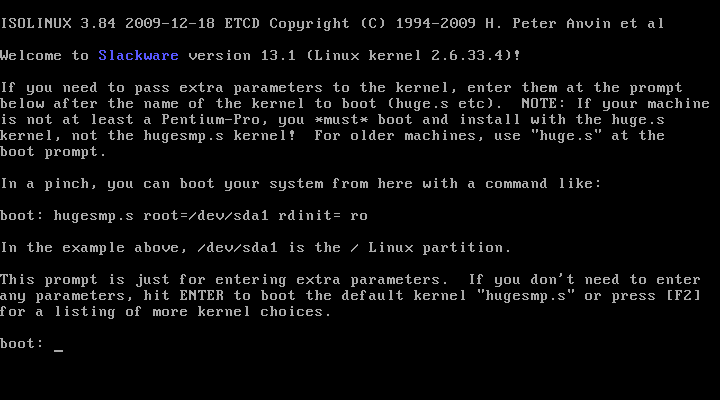
\includegraphics[scale=0.5]{images/09_home}
  \end{center}
  \caption{Voor het booten}
  \label{fig:home}
\end{figure}

Hier hoeft niets opgegeven te worden, er kan direct op enter gedrukt worden. Zodra er een  vraag wordt gesteld over de toetsenbord layout kan dit aangeven worden. Waarschijnlijk is het toetsenbord wat gebruikt wordt gewoon \emph{US-INTL}\footnote{Wanneer dit fout ingevult wordt kan dit later alsnog aangepast worden.} en kan er direct op enter gedrukt worden. Hierna dient er te worden ingelogd als ``root''. Type nu \texttt{setup}\index{setup}.

Zodra je setup hebt gekozen krijg wordt de fout uit figuur \ref{fig:fout} gegeven. Deze fout komt doordat er nog geen partities gemaakt zijn.
\begin{figure}[H]
  \begin{center}
    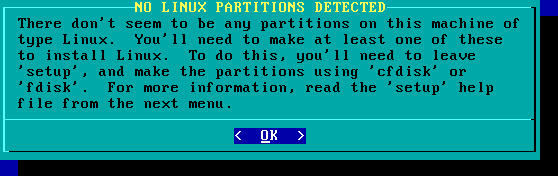
\includegraphics[scale=0.5]{images/08_installer_fout}
  \end{center}
  \caption{Fout bij het begin}
  \label{fig:fout}
\end{figure}

\section{fdisk}
Voordat we dus verder gaan moeten we eerst partities maken. Kies gewoon voor ``Ok'' en sluit de \emph{setup} af. Hierna kunnen we de partities als volgt aanmaken:
\begin{lstlisting}
fdisk /dev/sda
\end{lstlisting}
Waarbij \emph{/dev/sda} de harde schijf is welke gebruikt moet worden voor de \emph{Slackware} installatie. Voer de volgende commando's uit\footnote{Zie bijlage \ref{app.fdisk} voor meer informatie over \texttt{fdisk}\index{fdisk} en wat de onderstaande commando's/parameters betekenen.}:
\begin{lstlisting}
n
p
1
<default>
+10G
n
p
2
<default>
+14G
n
p
3
<default>
<default>
t
3
82
a
1
\end{lstlisting}
Controleer voordat de tabel wordt weggeschreven of dit klopt. Dit kan met de optie \emph{p}. Het zal overeen moeten komen met het onderstaande voorbeeld\footnote{Uiteraard er van uitgaande dat de harde schijf van dezelfde grote is. Controleer met de verhoudingen met de door jou gebruikte harde schijf.}:
\begin{lstlisting}
Command (m for help): p

Disk /dev/sda: 26.8 GB, 26843545600 bytes
255 heads, 63 sectors/track, 3263 cylinders, total 52428800 sectors
Units = sectors of 1 * 512 = 512 bytes
Sector size (logical/physical): 512 bytes / 512 bytes
I/O size (minimum/optimal): 512 bytes / 512 bytes
Disk identifier: 0x028f6a13

   Device Boot      Start         End      Blocks   Id  System
/dev/sda1   *        0       20973567    10485760   83  Linux
/dev/sda2        20973568    50333695    14680064   83  Linux
/dev/sda3        50333696    52428799     1047552   82  Linux swap
\end{lstlisting}
Wanneer het klopt kan de tabel met \emph{w} worden weggeschreven naar de schijf. De partitietabel is dan opgeslagen. \emph{Slackware} weet nu welke ruimte hij kan gebruiken. De installatie kan nu opnieuw gestart worden door het commando \texttt{setup} uit te voeren. 

\emph{Tip: Door de toets combinatie ``ctrl + page\_up'' en ``ctrl + page\_down'' kan door de terminal historie buffer gelopen worden}\index{historie}

\section{De installatie}
Nu begint de echte installatie van \emph{Slackware}. Het menu uit figuur \ref{fig:setup2} komt nu in beeld.
\begin{figure}[H]
  \begin{center}
    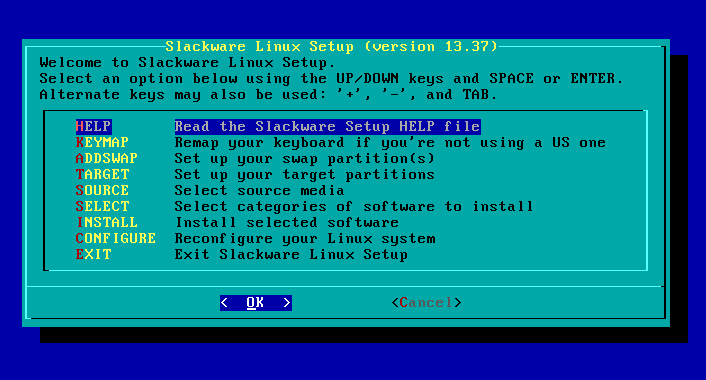
\includegraphics[scale=0.5]{images/01_installer}
  \end{center}
  \caption{Hoofdmenu van de installatie}
  \label{fig:setup2}
\end{figure}
De help functie hebben we niet nodig, omdat er al bekend is wat er gedaan moet worden. Het keyboard is ook al geconfigureerd, dus er kan gelijk gekozen worden voor de optie \emph{addswap}. Wanneer het bij \texttt{fdisk}\index{fdisk} goed is geconfigureerd zal hier \emph{/dev/sda3} weergeven worden. Kies hiervoor en druk op Ok. 

Er volgt nu een optie om op \emph{bad blocks} te controleren. In een \emph{VM} is dit niet nodig, bij fysieke hardware is het aan te raden om problemen te voorkomen. Hierna zal de \emph{swap} geactiveerd worden.

\subsection{Linux partities}
Er volgt nu een nieuw scherm, zoals te zien in figuur \ref{fig:partitie}\footnote{De waardes kunnen anders zijn, afhankelijk van de eerder gekozen waardes.}. \emph{Slackware} wil graag weten op welke partitie de \emph{root (/)} ge\"{i}nstalleerd kan worden. Kies hier voor \emph{/dev/sda1}, de kleinste van de twee. 

\begin{figure}[H]
  \begin{center}
    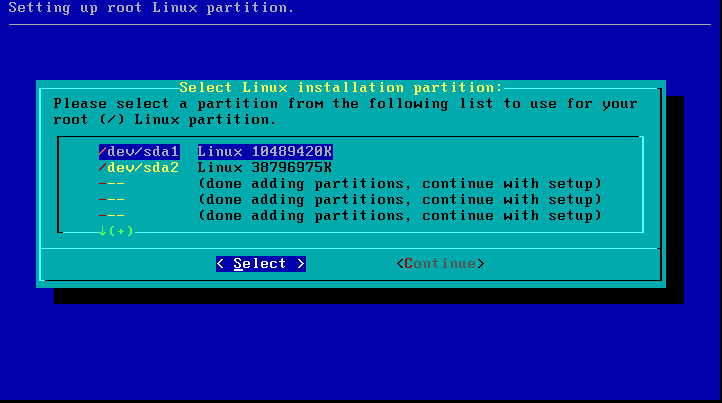
\includegraphics[scale=0.5]{images/02_partition}
  \end{center}
  \caption{Partities.}
  \label{fig:partitie}
\end{figure}

Bij de volgende stap moet het filesystem gekozen worden. Kies voor ``Format'' en in het volgende scherm het type, bijvoorbeeld \emph{EXT4}\index{EXT4}\footnote{Het gaat te ver om in dit document uitgebreid uit te leggen welke type file systems er zijn. \emph{EXT4} werkt in principe correct voor wat wij doen.}. Er kan nu weer een ``mount point'' worden gekozen. Kies hier voor \emph{/home}. Hierna zal er een overzicht te zien zijn, zoals figuur \ref{fig:fstab}.

\begin{figure}[H]
  \begin{center}
    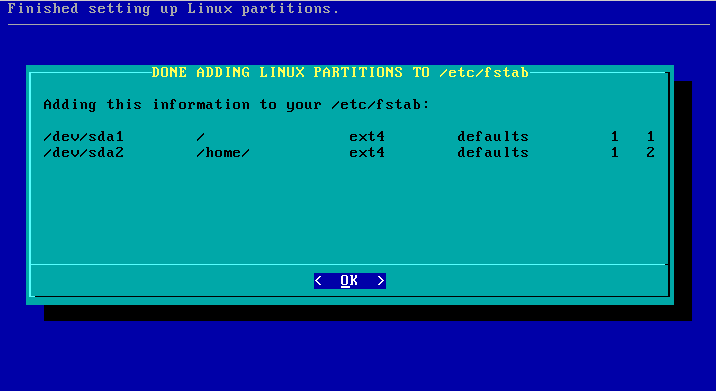
\includegraphics[scale=0.5]{images/03_fstab}
  \end{center}
  \caption{De gemaakte schijfindeling}
  \label{fig:fstab}
\end{figure}

\section{Packages}
De harde schijven zijn nu klaar voor gebruik en er kan begonnen met de installatie van het systeem. Zodra er op ``Ok'' wordt gedrukt zal er gevraagd worden om een locatie van de \emph{packages}. Kies hier voor \emph{FTP/HTTP}\footnote{CD is ook een mogelijkheid, alleen vereist het meer cd's}. Zie ook figuur \ref{fig:source}. 

\begin{figure}[H]
  \begin{center}
    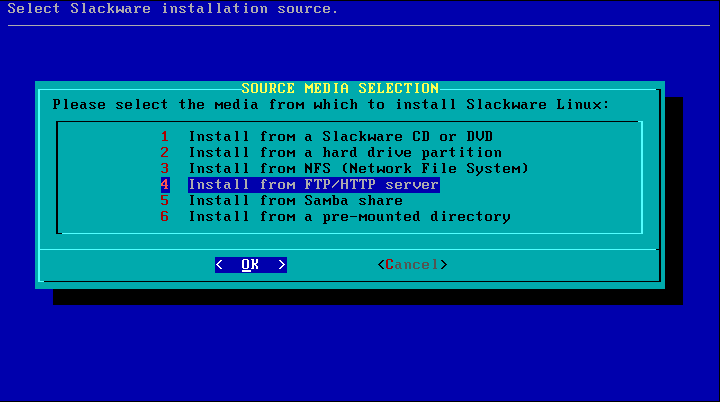
\includegraphics[scale=0.5]{images/04_source_media}
  \end{center}
  \caption{Source media keuze}
  \label{fig:source}
\end{figure}

Er zal nu worden gevraagd naar de netwerk configuratie. Dit is natuurlijk afhankelijk van de situatie. Bij het gebruik van \emph{VirtualBox} zal \emph{DHCP} voldoende zijn. Mocht je geen gebruik maken van \emph{Virtualbox} moet je de gegevens invullen welke voor het lokale netwerk gelden.

Er kan nu een \emph{mirror}\index{mirror} worden gekozen. Dit is een plek waar een kopie van alle \emph{Slackware} packages te vinden is. Een voorbeeld kan zijn \url{ftp://ftp.fu-berlin.de/}\footnote{Op de afbeelding is het IP van deze host te zien.}, zie ook \ref{fig:mirror}. Uiteraard kan ook een andere mirror gekozen worden. Zie hiervoor de \emph{Slackware} site.

\begin{figure}[H]
  \begin{center}
    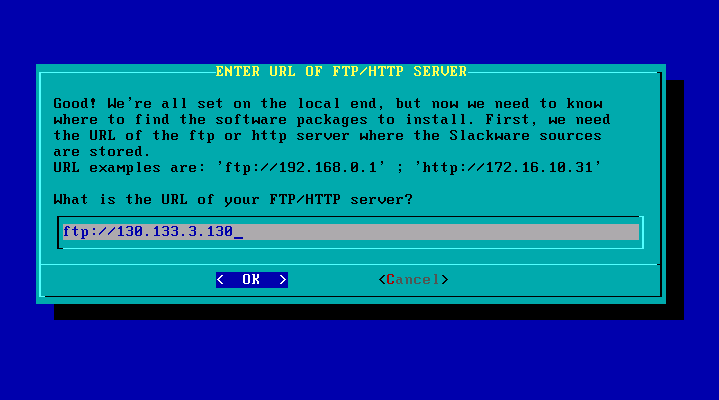
\includegraphics[scale=0.5]{images/05_mirror_location}
  \end{center}
  \caption{Mirror locatie}
  \label{fig:mirror}
\end{figure}

Nu zal er ook nog gekozen moeten worden voor een map op de \emph{mirror server}. Op het moment van schrijven is \emph{unix/linux/mirrors/slackware/slackware/} de goede directory. Dit kan bij het gebruik van een andere mirror een andere map zijn, dit is mirror afhankelijk. Zie hierbij ook figuur \ref{fig:mirror2}.

\begin{figure}[H]
  \begin{center}
    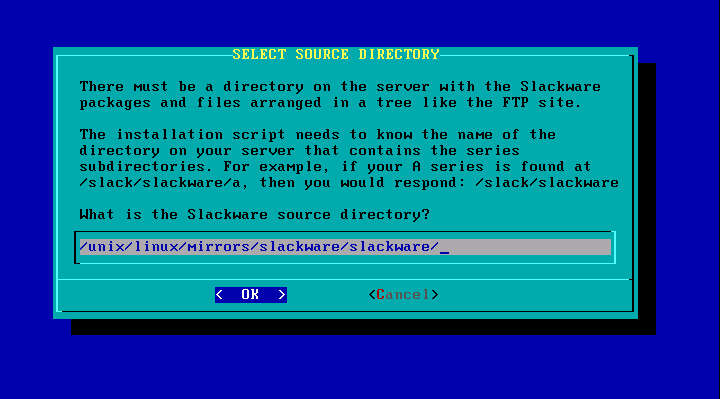
\includegraphics[scale=0.5]{images/06_mirror_location_2}
  \end{center}
  \caption{Mirror locatie}
  \label{fig:mirror2}
\end{figure}
\emph{Slackware} gaat nu controleren of de mirror gegevens kloppen en je krijgt de vraag of je het nogmaals wilt proberen of niet. Je kiest hier uiteraard voor niet.

In dit scherm kan er gespecificeerd worden welke packages ge\"{i}nstalleerd moeten worden. De volgende packages zijn niet nodig, wij willen namelijk geen \emph{GUI} gebruiken. Deselecteer dus de volgende opties: 
\begin{itemize}
  \item[1.] Linux kernel source\footnote{Deze optie is alleen nodig als er kernels compiled worden op de machine}
  \item[2.] KDE
  \item[3.] TEX
  \item[4.] X
  \item[5.] XAP
  \item[6.] Games
\end{itemize}
Kies nu weer ``Ok'', zoals te zien op figuur \ref{fig:packages}. 

\begin{figure}[H]
  \begin{center}
    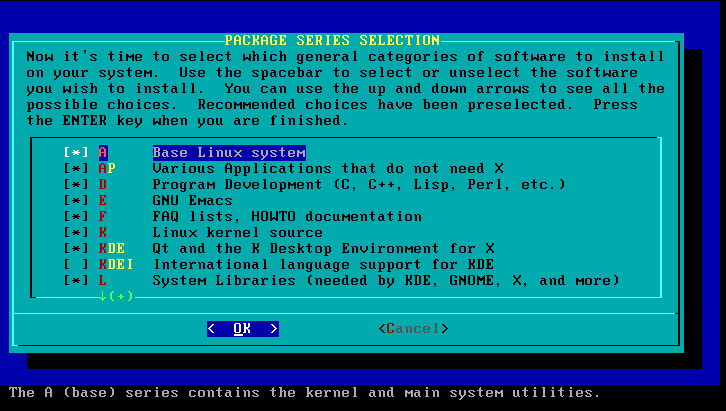
\includegraphics[scale=0.5]{images/07_package_select}
  \end{center}
  \caption{Packages}
  \label{fig:packages}
\end{figure}

Hierna krijg je het scherm zoals in figuur \ref{fig:install_full}. Het is aan te raden hier om ``full'' te kiezen, dit is de snelste optie en hoef je het minste te doen. Wanneer er een package vereist is om te installeren zal deze nu eerst automatisch van de gekozen \emph{mirror} afgehaald worden. Iedere package zal ook een korte beschrijving hebben welke op het scherm staat tijdens de installatie. Zodra \emph{Slackware} klaar is met alle packages op te halen en installeren gaat hij vanzelf verder met figuur \ref{fig:install_usb}. Op deze vraag kies je ``skip''.
\begin{figure}[H]
  \begin{center}
    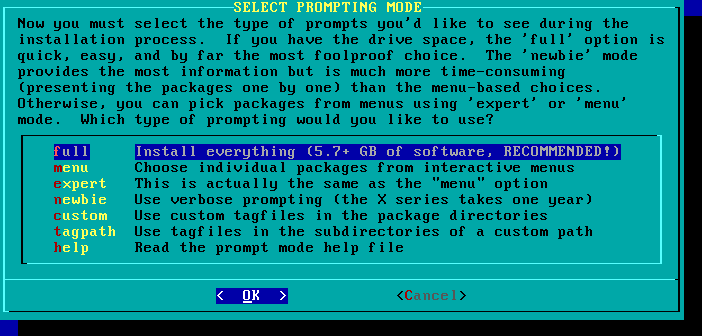
\includegraphics[scale=0.5]{images/install_full}
  \end{center}
  \caption{Installatie optie}
  \label{fig:install_full}
\end{figure}

\begin{figure}[H]
  \begin{center}
    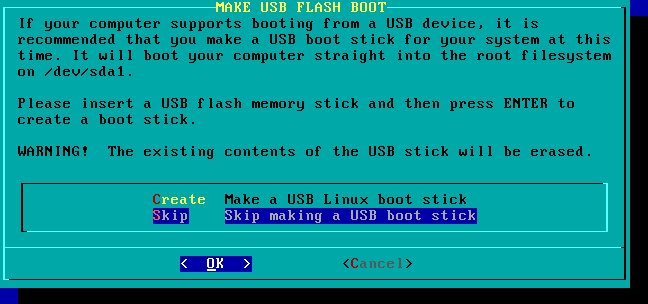
\includegraphics[scale=0.5]{images/install_usb}
  \end{center}
  \caption{USB opstart disk}
  \label{fig:install_usb}
\end{figure}


\section{LILO}
\begin{figure}[H]
  \begin{center}
    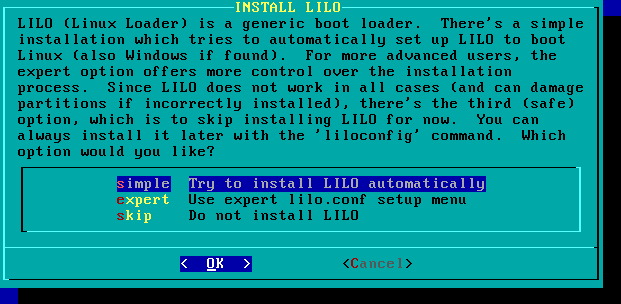
\includegraphics[scale=0.5]{images/install_lilo1}
  \end{center}
  \caption{LILO installatie}
  \label{fig:install_lilo1}
\end{figure}
\emph{LILO}\index{LILO} is de standaard bootmanager van \emph{Slackware}, \emph{LILO} is echter niet heel uitgebreid en je kan er niet veel mee. Hierom hebben wij ervoor gekozen om \emph{GRUB}\index{GRUB} te gaan gebruiken als bootmanager en gaan we deze later dan ook installeren. Maar voordat we dit kunnen, moeten we eerst een werkend systeem hebben en moet je dus \emph{LILO} installeren. 

In het scherm van \ref{fig:install_lilo1} moet je ``simple'' kiezen. Hierna krijg je het scherm uit figuur \ref{fig:install_lilo2}. Je kan hier de standaard instelling behouden.

\begin{figure}[H]
  \begin{center}
    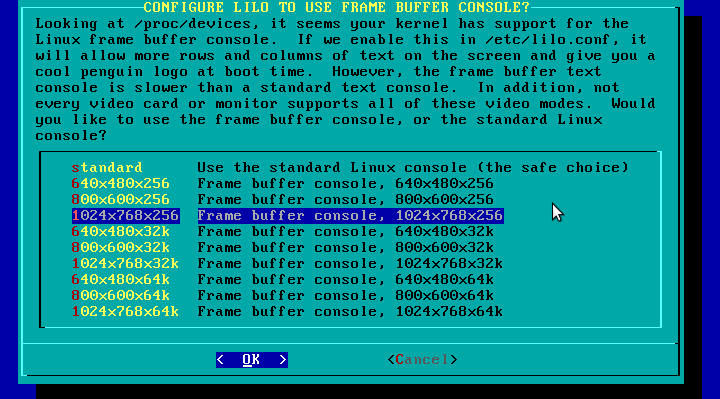
\includegraphics[scale=0.5]{images/install_lilo2}
  \end{center}
  \caption{LILO framebuffer}
  \label{fig:install_lilo2}
\end{figure}

\begin{figure}[H]
  \begin{center}
    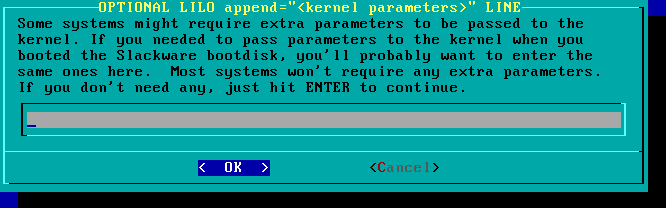
\includegraphics[scale=0.5]{images/install_lilo3}
  \end{center}
  \caption{LILO kernel options}
  \label{fig:install_lilo3}
\end{figure}
\begin{figure}[H]
  \begin{center}
    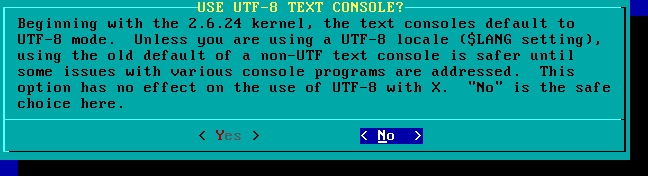
\includegraphics[scale=0.5]{images/install_lilo4}
  \end{center}
  \caption{LILO UTF8}
  \label{fig:install_lilo4}
\end{figure}
In sommige gevallen is het nodig om de kernel een aantal extra opties mee te geven om op te starten. Dit kan je in de installatie opgeven in \ref{fig:install_lilo3}. In principe hoef je hier niets op te geven en werkt het direct. Voor de echte instellingen krijgen we eerst nog een vraag over UTF8 zoals uit figuur \ref{fig:install_lilo4}. Je kan hier gewoon het standaard antwoord kiezen.

\begin{figure}[H]
  \begin{center}
    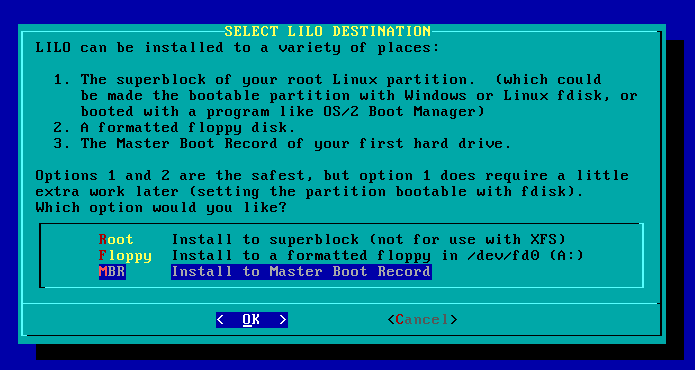
\includegraphics[scale=0.5]{images/install_lilo5}
  \end{center}
  \caption{LILO locatie}
  \label{fig:install_lilo5}
\end{figure}
In het scherm van figuur \ref{fig:install_lilo5} wordt gevraagd waar \emph{LILO} geinstalleerd moet worden. Je kan hier kiezen voor \emph{mbr}, de standaard keuze. In principe kan je ook kiezen voor \emph{root}, mits je de partitie als \emph{bootable} hebt ingesteld. Als je de instructies correct gevolgd heb was hij al bootable.

\section{Laatste configuratie}
Kies als muis voor een generieke \emph{PS2} muis. Dit zal de minste kans op problemen geven. 
Er zal ook nu weer om de netwerk configuratie gevraagd worden. Vul deze weer op de gewenste manier in. Vul als hostname een zelf gekozen naam in.

Op de vraag over welke \emph{services} geactiveerd moeten zijn kan er gewoon met ``Ok'' de default waardes worden bevestigd. Als tijdzone kan er natuurlijk gewoon ``Europe/Amsterdam'' worden gekozen, tenzij er een andere waarde gewenst is. 

Om het systeem veilig te kunnen gebruiken is het nodig om een \emph{root wachtwoord} op te geven. Dit wachtwoord is nodig om als hoofdgebruiker op het systeem in te kunnen loggen en zal dus een veilig en sterk wachtwoord moeten zijn. Onthoud en bescherm dit goed! 

Na een herstart (\texttt{reboot}\index{fdisk}) kan er ingelogd worden met ``root'' en het gekozen wachtwoord. 

\section{GRUB installatie}
De standaard bootloader van \emph{Slackware} is \emph{LILO}. Omdat \emph{GRUB} gemakkelijker en uitgebreider is, gaan we in dit dictaat gebruik maken van \emph{GRUB}.

\subsection{Downloaden en installeren GRUB}
In het geval van \emph{GRUB} bestaat er een standaard package om te installeren, maar staat deze enkel in ``extra''. Dit kunnen we vinden in de \emph{PACKAGES.TXT}\footnote{\url{ftp://ftp.fu-berlin.de/unix/linux/mirrors/slackware/slackware-13.1/extra/PACKAGES.TXT}}. Download de \emph{package}, en installeer deze: 
\begin{lstlisting}
root@slackbak:~# cd /tmp/
root@slackbak:/tmp# wget "ftp://ftp.fu-berlin.de/unix/linux/mirrors/slackware/slackware/extra/grub/grub-0.97-i486-9.txz"
root@slackbak:/tmp# installpkg grub-0.97-i486-9.txz 
\end{lstlisting}

\subsection{grubconfig}
\emph{GRUB} is nu ge\"{i}nstalleerd, maar nog niet geconfigureerd. Voordat \emph{GRUB} gebruik kan worden zal dat eerst gedaan moeten worden. Dit is echter erg eenvoudig:
\begin{lstlisting}
grubconfig
\end{lstlisting}
Hierna krijg je de zelfde soorten vragen als bij \emph{LILO}, je kan hier ook dezelfde antwoorden invullen.

De installatie is nu helemaal afgerond. Wanneer er gebruik wordt gemaakt van \emph{VirtualBox} is het aan te raden een kopie te maken van de harde schijf. Wanneer er dan iets fout gaat, kan simpelweg de kopie van de schijf worden teruggezet. Dit scheelt een herinstallatie van \emph{Slackware}. 

% tirlnx01 - Materiaal om het keuzevak Linux te geven 
% op de Hogeschool Rotterdam.
% Copyright (C) 2010 - 2011  Paul Sohier, Kevin van der Vlist
%
% This program is free software: you can redistribute it and/or modify
% it under the terms of the GNU General Public License as published by
% the Free Software Foundation, either version 3 of the License, or
% (at your option) any later version.
%
% This program is distributed in the hope that it will be useful,
% but WITHOUT ANY WARRANTY; without even the implied warranty of
% MERCHANTABILITY or FITNESS FOR A PARTICULAR PURPOSE.  See the
% GNU General Public License for more details.
%
% You should have received a copy of the GNU General Public License
% along with this program.  If not, see <http://www.gnu.org/licenses/>.
%
% Kevin van der Vlist - kevin@kevinvandervlist.nl
% Paul Sohier - paul@paulsohier.nl

\chapter{Het systeem}
Nu het systeem gereed is, kan er begonnen worden met werken in de installatie. Het begint natuurlijk met een inlog prompt: 
\begin{lstlisting}
slackbak login: 
\end{lstlisting}
Na de installatie is er maar \'{e}\'{e}n gebruiker beschikbaar, de zogenaamde \emph{root account}\index{root}. Het wachtwoord van deze gebruiker is opgegeven tijdens de installatie. Na het inloggen kan er begonnen worden met de configuratie van het systeem.

\section{root}
De gebruiker ``root'' heeft alle rechten op het systeem. Het is daarom erg gevaarlijk om onder dit account te werken. E\'{e}n verkeerd commando en het systeem is vernietigd\footnote{rm -rf /tmp/ vs rm -rf /tmp /}. Het ``root'' account dient daarom alleen gebruikt te worden wanneer dit noodzakelijk is. Als het dan toch gebruikt moet worden, maak dan gebruik van de volgende stappen\footnote{by Matt Welsh}:
\begin{itemize}
  \item[1.] Ga op je handen zitten.
  \item[2.] Denk na over wat je wilt doen.
  \item[3.] Typ de commando's in.
  \item[4.] Ga weer op je handen zitten.
  \item[5.] Denk na over de consequentie van het commando.
  \item[6.] Toets ``enter''.
  \item[7.] Log uit of ga naar 1.
\end{itemize}

Zo op het eerste gezicht zal dit misschien erg overtrokken overkomen. Iedere gebruiker die al wat langer met \emph{UNIX} werkt zal echter kunnen vertellen dat de bovenstaande procedure een echte \emph{lifesaver} is. De meeste mensen hebben wel een keer meegemaakt dat ze iets uitvoerden waar ze na het intoetsen van ``enter'' al spijt van hadden.

\subsection{root worden}
Om root te worden volstaat het om het commando \texttt{su}\index{su} in te typen in de shell. Er zal nu om het wachtwoord gevraagd worden. Als dit goed is, zal de gebruiker een onbeperkte shell gepresenteerd krijgen. 

\section{Reboot, Shutdown \& Runlevels}
Ook een \emph{Linux} systeem dient natuurlijk op een correcte manier gestart en gestopt te worden. Dit kan echter wel op verschillende manieren. Achter de schermen gebeurt er meestal hetzelfde, zoals het \emph{flushen} van openstaande buffers naar de \emph{harde schijf}, of het netjes afsluiten van draaiende \emph{services}. Het afsluiten kan op de volgende manieren: 
\begin{itemize}
  \item[1.] \texttt{init 0}\index{init}
  \item[2.] \texttt{halt}\index{halt}
  \item[3.] \texttt{shutdown}\index{shutdown}
\end{itemize}

Een \emph{reboot} kan op de volgende manieren:
\begin{itemize}
  \item[1.] \texttt{init 6}\index{init}
  \item[2.] \texttt{reboot}
  \item[3.] \texttt{shutdown -r}
\end{itemize}

De reden dat dit op verschillende manier gedaan kan worden heeft te maken met de geschiedenis van \emph{Linux}. Wanneer \texttt{shutdown}\index{shutdown} wordt aangeroepen, zal er eerst een \emph{SIGTERM} signal verstuurd worden naar alle processen. Ook zal login \emph{blocking} worden en zullen gebruikers genotificeerd worden dat het systeem down gaat. De \emph{shutdown} of \emph{reboot} word dus aangekondigd. Hierna wordt er achter de schermen aan init gevraagd om het \emph{runlevel} te wijzigen naar het gevraagde niveau. Wanneer er gebruik gemaakt wordt van \texttt{halt}\index{halt} zal er direct een \emph{SIGKILL} signal naar de actieve processen gestuurd worden. Aangezien dit signal niet door het proces zelf kan worden genegeerd, krijgen actieve processen geen kans om gebruikers nog dingen te vragen\footnote{Een duidelijk voorbeeld is het afsluiten wanneer een \emph{tekst editor} nog data heeft die nog niet is opgeslagen. Er zal nu geen dialoog worden getoond met de vraag of er nog moet worden opgeslagen}. Dit kan resulteren in dataverlies. Tegenwoordig zal een aanroep aan halt standaard worden doorgewezen naar shutdown, omdat dit gebruiksvriendelijker is en beter voor de consistentie van het systeem. Het zal immers een unieke gelegenheid zijn als men geen gebruik wilt maken van een nette afsluit procedure. Tegenwoordig dient er om dat doel te bereiken dan ook een speciale \emph{flag} mee worden gegeven aan \texttt{halt}\index{halt}:
\begin{lstlisting}
kevin@slackbak:~$ man halt
[..]
       -f     Force halt or reboot, don't call shutdown(8).
\end{lstlisting}%$ 

Als laatste is er \texttt{init}\index{init}, welke direct de \emph{runlevels} modificeerd. Een \emph{runlevel} is een gevolg van een \emph{System V} gebaseerde systeem initialisatie. Ieder \emph{runlevel} heeft bepaalde taken die in dat niveau worden uitgevoerd. \emph{Slackware} maakt gebruik van de volgende \emph{runlevels}: 

\begin{tabular}[t]{ll}
  \hline
  Runlevel & Taken\\
  \hline
  0 & Halt het systeem\\
  1 & Single user mode\\
  2,3 & Multi User Mode - Default\\
  4 & 3 + X11\\
  6 & Reboot het systeem\\
\end{tabular}

\section{Aanmaken van gebruikers}
\emph{Linux} is een zogenaamd \emph{multi-user} operating system. Dit betekent dat meerdere gebruikers gemakkelijk van hetzelfde systeem gebruik kunnen maken. Dit kan zijn via netwerk gerelateerde diensten als remote terminals zoals \emph{ssh}\index{ssh}, maar ook met meerdere hardware sets, zodat er meerdere werkplekken op een systeem ontstaan. 

Voordat er van het bovenstaande gebruik gemaakt kan worden, zal een gebruiker eerst een \emph{account} moeten krijgen op een systeem. Dit kan met behulp van het commando \texttt{adduser}\index{adduser}.
\begin{lstlisting}
root@slackbak:/home/kevin# adduser klaasvaak
Login name for new user: klaasvaak
User ID ('UID') [ defaults to next available ]: 
Initial group [ users ]: 
Additional UNIX groups:
[...]
: 
Home directory [ /home/klaasvaak ] 
Shell [ /bin/bash ] 
Expiry date (YYYY-MM-DD) []: 
New account will be created as follows:
---------------------------------------
Login name.......:  klaasvaak
UID..............:  [ Next available ]
Initial group....:  users
Additional groups:  [ None ]
Home directory...:  /home/klaasvaak
Shell............:  /bin/bash
Expiry date......:  [ Never ]
\end{lstlisting}

\section{Terminals}
Het inloggen in \emph{Linux} gebeurt in een terminal. Standaard wordt er gestart met terminal 1. Toets ``alt + F2'' en terminal 2 verschijnt. Standaard start \emph{Slackware} zes terminals. Zes verschillende of dezelfde gebruikers kunnen tegelijk ingelogd zijn. Een terminal heet \emph{tty}:\index{tty}

\begin{lstlisting}
kevin@slackbak:~$ ps -ef | grep tty
kevin 1585 1 0 20:32 tty1 00:00:00 -bash
root  1586 1 0 20:32 tty2 00:00:00 /sbin/agetty 38400 tty2 linux
root  1587 1 0 20:32 tty3 00:00:00 /sbin/agetty 38400 tty3 linux
root  1588 1 0 20:32 tty4 00:00:00 /sbin/agetty 38400 tty4 linux
root  1589 1 0 20:32 tty5 00:00:00 /sbin/agetty 38400 tty5 linux
root  1590 1 0 20:32 tty6 00:00:00 /sbin/agetty 38400 tty6 linux
\end{lstlisting}%$
Hier is een overzicht te zien van alle \emph{processen} die zijn gerelateerd aan de \emph{tty}. \texttt{agetty}\index{agetty} is een proces wat ervoor zorgt dat er een nieuwe \emph{tty} verbinding kan worden geopend. Hierna zal er een login prompt worden gestart. Er kan dan worden ingelogd op de \emph{terminal}. In het bovenstaande voorbeeld is te zien dat op de tweede \emph{tty} een gebruiker met de naam ``kevin'' is ingelogd. Deze maakt gebruik van de \emph{Bash} shell. \index{Bash}

\section{Mountpoint}
Tijdens het starten van \emph{Linux} worden er automatisch bepaalde partities beschikbaar gemaakt. Dit wordt \emph{mounten} genoemd. Deze automatische \emph{mounts} komen uit een speciale file, namelijk \emph{/etc/fstab}. Deze config file bevat dus de zogenaamde \emph{statische mountpoints}. Wanneer er een bepaalde partitie, bijvoorbeeld \emph{root (/)} \emph{gemount} moet worden, zal dit gedefini\"{e}erd moeten zijn in \emph{fstab}. Een voorbeeld van deze file is hieronder te zien: \index{fstab}\index{/}\index{/etc/fstab}
\begin{lstlisting}
kevin@slackbak:~$ cat /etc/fstab
/dev/sda1   /             ext4     defaults         1   1
/dev/sda2   /home         ext4     defaults         1   2
/dev/fd0    /mnt/floppy   auto     noauto,owner     0   0
devpts      /dev/pts      devpts   gid=5,mode=620   0   0
proc        /proc         proc     defaults         0   0
tmpfs       /dev/shm      tmpfs    defaults         0   0
/dev/sda3   swap          swap     sw               0   0
\end{lstlisting}%$
Hier valt dus te zien dat de eerste partitie van de eerste schijf met type \emph{EXT4} automatisch met default mount opties wordt gemount op de root van het systeem. Zo geldt het ook voor de andere regels. De mountpoints \emph{devpts}, \emph{proc} en \emph{tmpfs} zijn speciale mounts. 

\subsection{Devpts}\index{devpts}
Dit mountpoint bevat alle \emph{pseudo terminals} die geassocieerd zijn met het systeem. Alle programmatuur die gebruik maakt van input en output van userdata (\emph{ssh} en consorten) zal van input devices moeten lezen en naar output devices moeten schrijven. Deze \emph{pseudo terminals} zijn virtual devices die in deze behoefte voorzien. Een \emph{ssh}\index{ssh} sessie registreert bijvoorbeeld een virtueel toetsenbord, dat door \emph{Bash} gebruikt kan worden om input te lezen. Om een wildgroei (en een limiet aan \emph{pseudo devices}) te voorkomen is er een speciale \emph{multiplexer} geschreven welke de afhandeling van alle \emph{pseudo devices} regelt. Dit gebeurt binnen het \emph{devpts} filesystem. 

\subsection{Proc}\index{proc}
Dit mountpoint is een manifestatie van interne datastructuren van de \emph{Linux} kernel. Dit is duidelijker te maken met een voorbeeld:
\begin{lstlisting}
kevin@slackbak:~$ ps -ef | grep udevd
root 1016 1 0 13:49 ? 00:00:00 /sbin/udevd --daemon
kevin@slackbak:~$ cat /proc/1016/cmdline 
/sbin/udevd--daemon
kevin@slackbak:~$ cat /proc/version 
Linux version 2.6.33.4-smp (root@midas) (gcc version 4.4.4 (GCC) ) #2 SMP Wed May 12 22:47:36 CDT 2010
\end{lstlisting}%$
Hier is dus te zien dat de \emph{command line argumenten} van draaiende processen terug te vinden is in het \emph{proc} file system. Veel ervan is read-only, maar sommige kernel variabelen zijn te veranderen door te schrijven naar de speciale files binnen \emph{proc}.

\subsection{Tmpfs}\index{tmpfs}
Het \emph{mountpoint} \emph{tmpfs} staat voor \emph{temporary file system}. Sinds kernel versie 2.4 en groter is dit speciale type file system beschikbaar. Het bestaat uit gealloceerde \emph{memory pages}. De hoevelheid \emph{pages} kan dynamisch groeien indien gewenst. Een andere optimalisatie is dat weinig gebruikte \emph{pages} door de \emph{memory manager} naar de \emph{swap space}\index{swap} verplaatst kunnen worden. Ze zullen dus niet onnodig in het \emph{RAM}\index{RAM} blijven zitten. Dit filesystem kan worden gebruikt om data ``op te slaan'', maar toch in het geheugen te kunnen bewerken. Denk bijvoorbeeld aan tijdelijke opslag. 

\subsection{Swap}\index{swap}
\emph{Swap space} is secundaire memory space voor de \emph{Linux} kernel. Dit wordt gebruikt wanneer de hoeveelheid beschikbaar \emph{RAM} te klein wordt. Er kan dan uitgeweken worden naar de \emph{swap space}. De \emph{swap} is een speciaal geformatteerde partitie, of speciale file \emph{op} een partitie, welke gebruikt kan worden om ongebruikte \emph{memory pages} weg te schrijven. De \emph{swap} is wel merkbaar trager als het \emph{RAM} geheugen. Er moet dus voorkomen worden in veel gevallen dat de \emph{swap} gebruikt wordt.

\subsection{Mount}

Zelf een \texttt{mount}\index{mount} actie uitvoeren is erg simpel. Dit kan bijvoorbeeld als volgt: 
\begin{lstlisting}
mount -t vfat /dev/sdb1 /mnt/usbstick
\end{lstlisting}
Nu wordt \emph{device sdb, partitie 1} door \texttt{mount}\index{mount} aan \emph{/mnt/usbstick} gekoppeld. Het type van het \emph{file system} is expliciet opgegeven als zijnde \emph{FAT}. Dit is niet altijd nodig, aangezien moderne implementaties van \texttt{mount}\index{mount} zelf kunnen bepalen wat het type \emph{file system} is. Het weglaten van de optie '-t' volstaat dan. 

Met \texttt{mount} valt te zien welk \emph{file systems} momenteel \emph{gemount} zijn. Zoals te zien is staat de usb stick er ook bij:
\begin{lstlisting}
kevin@slackbak:~$ mount
/dev/root on / type ext4 (rw,relatime,barrier=1,data=ordered)
proc on /proc type proc (rw)
sysfs on /sys type sysfs (rw)
usbfs on /proc/bus/usb type usbfs (rw)
/dev/sda2 on /home type ext4 (rw)
tmpfs on /dev/shm type tmpfs (rw)
/dev/sdb1 on /mnt/usbstick type vfat (rw)
\end{lstlisting}%$
\texttt{umount}\index{umount} kan worden gebruikt om het \emph{mounted file system} te ontkoppelen. Het device is dan dus niet meer beschikbaar voor het systeem: 
\begin{lstlisting}
umount /mnt/usbstick
\end{lstlisting}
Hierna kan via \texttt{mount} gecontroleerd worden of dit ook echt het geval is.

\section{Slackware Package}
Alle ge\"{i}nstalleerde software is tijdens de installatie van internet gehaald. Wanneer er bepaalde pakketten vervangen moeten worden, of als er nieuwe software ge\"{i}nstalleerd moet worden kan dit op twee manieren. Het gewenste pakket kan van de \emph{Slackware} website of van de \emph{Slackware cd-rom} gehaald worden en met de \emph{package manager} ge\"{i}nstalleerd worden. Een andere manier is de software in \emph{source-code} vorm te installeren. Voor meer informatie over de \emph{Slackware package manager} zie bijlage \ref{app.package} en voor \emph{source-code installatie} zie bijlage \ref{app.source}.

\section{De man pages}\label{man}
E\'{e}n van de belangrijkste commando's op het systeem is \texttt{man}\index{man}\cite{bib.man}\cite{bib.ldp}. Dit commando geeft een \emph{manual} over een programma weer. Hier is in te vinden wat het programma doet en hoe het werkt. Mocht iets niet duidelijk zijn dan is met \texttt{man}\index{man} altijd meer uitleg te vinden:
\begin{lstlisting}
man man
\end{lstlisting}
Dit is alles wat er over het commando bekend moet zijn. De parameter \emph{man} zorgt dat de \emph{manual} van het programma \texttt{man} geopend wordt. Deze \emph{manuals} zijn op een vaste manier opgebouwd, de structuur is bij iedere andere \emph{manual} terug te zien. 
\begin{itemize}
  \item[1] \emph{TITLE}: Bovenaan de pagina staat de titel van de pagina en welke \emph{manual} wordt weergeven\footnote{Er kunnen meerdere manual pages voor een titel zijn: \texttt{man open}\index{man} en \texttt{man 3 open}\index{man}}. In dit geval is het \emph{man(1)}.
  \item[2] \emph{NAME}: Nogmaals de naam van het commando en eventuele synoniemen en een korte omschrijving.
  \item[3] \emph{SYNOPSIS}: De \emph{synopsis} of \emph{syntax} is de manier waarop het commando gebruikt dient te worden. In het geval van \texttt{man} is dit \texttt{man [acdfFhkKtwW] [-m system] [-o string] [-C config\_file] [-M path] [-P pager] [-S section\_list] [section name] \ldots}\index{man}. Alle delen tussen de haken ``[ ]''  zijn eventuele opties. Wanneer deze worden weggelaten ontstaat er \texttt{man name}\index{man}. Dit is te testen door bijvoorbeeld \texttt{man man}\index{man} of \texttt{man ls}\index{man}.
  \item[4] \emph{DESCRIPTION}: Is een uitgebreidere omschrijving van de mogelijkheden van het commando.
  \item[5] \emph{OPTIONS}: Hier worden alle mogelijke \emph{configuratie switches} van het commando beschreven.
  \item[6] \emph{SEE ALSO}: Is een overzicht van verwante commando's.
\end{itemize}
De \emph{manual page} wordt weergeven door middel van het programma \texttt{less}\index{less}. Afsluiten kan met \emph{q}. Voor meer info, \texttt{man less}\index{man}.

Wanneer er voortaan ``naar de documentatie'' wordt verwezen zal, tenzij nader gespecificeerd, de \emph{man page} van het betreffende onderwerp bedoeld worden. 

\section{Libraries}
\emph{Libraries}, of \emph{bibliotheken} zijn bestanden die verschillende \emph{functies} of \emph{subroutines} bevatten die kunnen worden gebruikt door andere software. Op deze manier kan een systeem op een plek bepaalde \emph{libaries} met taken aanbieden, welke dan door de rest van het systeem kunnen worden gebruikt. Niet ieder programma dat een bepaalde taak wil uitvoeren hoeft dan het wiel opnieuw uit te vinden. Het kan dan juist gebruik maken van de logica die al te vinden is in de aanwezige \emph{libraries}. 

In de loop van de tijd zijn er enorm veel \emph{libaries} ontstaan. Als eerste komt dit omdat het ontwikkelen van applicaties veel sneller gaat. Ontwikkelaars kunnen immers code gebruiken die al bepaalde problemen oplost. 

Een tweede oorzaak is de delegatie van verantwoordelijkheid. Wanneer ieder programma wat data moet \emph{comprimeren} gebruik kan maken van dezelfde \emph{libary} zal dit allemaal dezelfde typen bestanden opleveren. Dit is erg gemakkelijk in gebruik, het ontwikkelteam van de \emph{libaries} kan er vervolgens zorgen dat dit formaat bruikbaar blijft. Mochten er fouten gevonden worden in de implementatie, dan hoeft dit ook maar op \'{e}\'{e}n plek te worden opgelost, niet in ieder los programma wat wil comprimeren. 

\subsection{Static libraries}
Een \emph{static library}, of \emph{statische bibliotheek} is een \emph{libary} die tijdens de \emph{compilatie} van een programma wordt \emph{gelinkt}. Dit betekend dat de benodigde delen van de \emph{libary} worden samengevoegd met het programma. 

\subsection{Shared libraries}
In tegenstelling tot \emph{static libaries} zijn \emph{shared libaries} niet tijdens de \emph{compilatie} samengevoegd, maar zullen tijdens het draaien van een programma worden geopend indien nodig. 

Dit gedrag heeft vele voordelen, maar de belangrijkste zijn ruimtebesparing en verminderd onderhoud. 

In het geval van ruimte besparing is dit te verklaren doordat ieder programma geen eigen kopie van een bepaalde \emph{libary} hoeft te hebben. De programma's zijn netto dus kleiner. 

De verbetering op het gebied van \emph{onderhoud} komt voort uit de gevolgen van de \emph{static libaries}. Mocht er een nieuwere versie van een \emph{libaryk} uitkomen omdat die veiligheidsfouten herstelt, zal dat betekenen dat ieder programma opnieuw \emph{gelinked} moet worden aan de \emph{libary}. 

Wanneer een \emph{libary} niet \emph{static}, maar \emph{shared} is kan er eenvoudig weg een upgrade van de betreffende \emph{libary} worden geupgrade. Hierna zal ieder programma gebruik gaan maken van de nieuwe versie, zodra dit programma herstart is. Het hele systeem is dus gelijk veilig. 

\subsubsection{ldconfig}
Om te zorgen dat een systeem een idee heeft over de beschikbare \emph{shared libary} wordt er gebruik gemaakt van het configuratiebestand \emph{ld.so.conf}, te vinden in \emph{/etc/}. 

Dit bestand wordt door \texttt{ldconfig}\index{ldconfig} gelezen, waarna er een cache met beschikbare \emph{libaries} wordt gemaakt. Deze cache kan worden gebruikt door het systeem om programma's de \emph{shared libary} te geven waar ze om vragen. 

Het commando \texttt{ldconfig}\index{ldconfig} leest sowieso de vertrouwde \emph{libary} mappen \emph{/lib} en \emph{/usr/lib} uit, en zal vervolgens in het bestand \emph{/etc/ld.so.conf} kijken waar het nog meer naar \emph{libaries} moet kijken. 

Mocht er dus een map met \emph{libaries} worden toegevoegd aan het systeem zal dat in dit bestand moeten gebeuren. Dit is erg eenvoudig, het bestand bevat alleen regels met locaties:
\begin{lstlisting}
kevin@slackbak:~$ cat /etc/ld.so.conf 
/usr/local/lib
/usr/i486-slackware-linux/lib
/usr/lib/seamonkey
\end{lstlisting}%$
Een nieuwe locatie is dus snel toegevoegd. 

% tirlnx01 - Materiaal om het keuzevak Linux te geven 
% op de Hogeschool Rotterdam.
% Copyright (C) 2010 - 2011  Paul Sohier, Kevin van der Vlist
%
% This program is free software: you can redistribute it and/or modify
% it under the terms of the GNU General Public License as published by
% the Free Software Foundation, either version 3 of the License, or
% (at your option) any later version.
%
% This program is distributed in the hope that it will be useful,
% but WITHOUT ANY WARRANTY; without even the implied warranty of
% MERCHANTABILITY or FITNESS FOR A PARTICULAR PURPOSE.  See the
% GNU General Public License for more details.
%
% You should have received a copy of the GNU General Public License
% along with this program.  If not, see <http://www.gnu.org/licenses/>.
%
% Kevin van der Vlist - kevin@kevinvandervlist.nl
% Paul Sohier - paul@paulsohier.nl

\chapter{Inrichting}
Dit hoofdstuk gaat over de schijf indeling van een \emph{Linux} systeem. We bedoelen niet het type \emph{file system} waarmee de harde schijf is ingedeeld, maar juist de structuur die wordt gebruikt om data \emph{op} de schijf te benaderen. Er zijn hier strikte richtlijnen voor opgesteld. Het volgen van deze richtlijnen wordt dan ook door veel \emph{distributies} gevolgd, al zijn er soms kleine implementatieverschillen. 

\section{Inleiding}
Om door een \emph{file system} heen te kunnen navigeren is het handig dat de basis navigatie bekend is bij de lezer. Lees daarom minimaal de \emph{NAME} en de \emph{DESCRIPTION} uit de \emph{manual} van de volgende commando's:
\begin{itemize}
  \item[1.] \texttt{cd}\index{cd} - \textbf{C}hange \textbf{D}irectory
  \item[2.] \texttt{cp}\index{cp} - \textbf{C}o\textbf{p}y
  \item[3.] \texttt{ls}\index{ls} - \textbf{L}i\textbf{s}t
  \item[4.] \texttt{mkdir}\index{mkdir} - \textbf{M}a\textbf{k}e \textbf{Dir}ectory
  \item[5.] \texttt{pwd}\index{pwd} - \textbf{P}rint \textbf{W}orking \textbf{D}irectory
  \item[6.] \texttt{rm}\index{rm} - \textbf{R}e\textbf{m}ove
  \item[7.] \texttt{rmdir}\index{rmdir} - \textbf{R}e\textbf{m}ove \textbf{Dir}ectory
  \item[8.] \texttt{df}\index{df} - \textbf{D}isk \textbf{F}ree
\end{itemize}

\section{Linux Standard Base}
De \emph{Linux Standard Base}, of \emph{LSB}\index{LSB}\cite{bib.lsb}, is een standaard die binnen de \emph{Linux} wereld is opgestart. Men wilde hiermee een duidelijke richtlijn specificeren over de volgende onderwerpen:
\begin{itemize}
  \item[1.] \emph{ELF}\footnote{\emph{Executeable and Linking Format - Binary interface standaard}} specificatie.
  \item[2.] Standaard \emph{libraries}. 
  \item[3.] Standaard \emph{commando's}. 
  \item[4.] \emph{File System hi\"{e}rarchie}. 
  \item[5.] \emph{Lokalisatie} mogelijkheden van binaries.
  \item[6.] \emph{Systeem initialisatie}\footnote{\emph{Run levels}, \emph{init scripts}, \ldots}.
  \item[7.] \emph{User} en \emph{groep} definities.
  \item[8.] Print framework\footnote{\emph{CUPS}}.
  \item[9.] \emph{Interpreters}\footnote{\texttt{python}\index{python}, \texttt{perl}\index{perl}, \ldots}.
  \item[10.] Basis \emph{X Window} systeem.
\end{itemize}
De meeste punten resulteren in droge opsommingen over wat er precies aanwezig moet zijn op een systeem. De informatie is duidelijk gedocumenteerd, zodat dit zelf opgezocht kan worden wanneer het nodig is. Het is echter wel handig om te weten hoe punt \emph{4} precies in elkaar zit. Dit heeft namelijk veel praktische gevolgen voor het gebruik van een \emph{LSB}-gecertificeerd systeem. 

\section{File System Hi\"{e}rarchie}
Een \emph{Linux} \emph{file systeem} is te representeren als een grote boom. De root node van deze tree is \emph{/}, welke 0-n\footnote{n is afhankelijk van het filesystem. \emph{EXT3} heeft bijvoorbeeld een limiet van 31998.} verschillende \emph{child nodes}\footnote{Directe kinderen, dus bestanden of mappen \emph{in} een \emph{parent}, een map.} bevat. Deze \emph{child nodes} kunnen zelf ook weer \emph{child nodes} hebben. Dit is te visualiseren in figuur \ref{fs_tree}. Hier is een bepaalde \emph{node} \emph{kevin} te zien, welke dus een diepte niveau van 3 heeft.
\begin{itemize}
  \item[1.] \emph{/}
  \item[2.] \emph{/home}
  \item[3.] \emph{/home/kevin}
\end{itemize}

\begin{figure}[H]
  \setlength{\unitlength}{1mm}
  \begin{center}
    \begin{picture}(90, 50)
      \thicklines
      % lvl 0
      % Root node
      \put(30,45){\circle{15}}
      \put(30,45){\makebox(0,1){\texttt{/}}}
      % Arrows
      \put(30,38){\vector(-3,-2){10}}
      \put(30,38){\vector(3,-2){10}}

      % lvl 1
      % usr
      \put(15,25){\circle{15}}
      \put(15,25){\makebox(0,1){\texttt{usr}}}
      % Arrows
      \put(15,18){\vector(-3,-2){10}}
      % home
      \put(45,25){\circle{15}}
      \put(45,25){\makebox(0,1){\texttt{home}}}
      % Arrows
      \put(45,18){\vector(-3,-2){10}}
      \put(45,18){\vector(0,-2){5}}
      \put(45,18){\vector(3,-2){10}}

      % lvl 2
      % usr/bin
      \put(0,5){\circle{15}}
      \put(0,5){\makebox(0,1){\texttt{bin}}}
      % home/femke
      \put(30,5){\circle{15}}
      \put(30,5){\makebox(0,1){\texttt{femke}}}
      % home/kevin
      \put(45,5){\circle{15}}
      \put(45,5){\makebox(0,1){\texttt{kevin}}}
      % home/paul
      \put(60,5){\circle{15}}
      \put(60,5){\makebox(0,1){\texttt{paul}}}
    \end{picture}
  \end{center}
  \caption{Een file system tree}
  \label{fs_tree}
\end{figure}

Alle \emph{nodes} op niveau 2 hebben echter een speciale betekenis. Ze bevatten allemaal \emph{content} die aan hun beschrijving voldoet. Dit maakt het gemakkelijk en voorspelbaar om bepaalde kritieke bestanden te vinden, te gebruiken of aan te passen. Een goed voorbeeld om duidelijk te maken wat er precies bedoeld wordt zijn configuratie bestanden. Deze zijn in principe altijd in \emph{/etc} terug te vinden. De volgende \emph{directories} zijn beschreven met hierbij hun doel:

\begin{tabular}[t]{ll}
  \hline
  Directory & Beschrijving\\
  \hline
  /bin & Basis user-gerelateerde programma's en scripts, zoals \texttt{ls}\index{ls}.\\
  /boot & \emph{Bootloader} (\emph{LILO}, \emph{GRUB}) files.\\
  /dev & \emph{Block-,} en \emph{Character devices}.\\
  /etc & Configuratie en systeem initialisatie.\\
  /home & Gebruikersmappen (geen \emph{root}).\\
  /lib & Belangrijke libraries (\emph{kernel} modules, \emph{libc}).\\
  /mnt & Directory voor generieke \emph{mountpoints}.\\
  /opt & Optionele packages. \emph{Slackware} installeert \emph{KDE} hier.\\
  /proc & \emph{Proc} filesystem voor \emph{kernel} datastructuren.\\
  /root & \emph{Root's} home directory.\\
  /sbin & Systeem programma's, nodig voor startup of \emph{root}.\\
  /tmp & Tijdelijke bestanden, iedereen heeft lees + schrijf rechten hier.\\
  /usr & Gebruikers-gerelateerde programma's (browser, \emph{X11}, \ldots).\\
  /var & Systeem log files, \emph{lock files}, \emph{mail spools} en \emph{printer spools}.\\
\end{tabular}

Als tradities had de ``root'' user zijn home directory oorspronkelijk in \emph{/}, maar veel distributies gebruiken tegenwoordig \emph{/root/}\cite{bib.root}. Dit heeft dus oorspronkelijk niets te maken met de beveiliging van het systeem.

% tirlnx01 - Materiaal om het keuzevak Linux te geven 
% op de Hogeschool Rotterdam.
% Copyright (C) 2010 - 2011  Paul Sohier, Kevin van der Vlist
%
% This program is free software: you can redistribute it and/or modify
% it under the terms of the GNU General Public License as published by
% the Free Software Foundation, either version 3 of the License, or
% (at your option) any later version.
%
% This program is distributed in the hope that it will be useful,
% but WITHOUT ANY WARRANTY; without even the implied warranty of
% MERCHANTABILITY or FITNESS FOR A PARTICULAR PURPOSE.  See the
% GNU General Public License for more details.
%
% You should have received a copy of the GNU General Public License
% along with this program.  If not, see <http://www.gnu.org/licenses/>.
%
% Kevin van der Vlist - kevin@kevinvandervlist.nl
% Paul Sohier - paul@paulsohier.nl

\chapter{Editors}
Op een \emph{Linux} systeem zijn er verschillende \emph{editors}, ofwel tekstverwerkers beschikbaar. De verschillende \emph{editors} hebben allemaal een eigen doelgroep. Zo zijn er \emph{editors} die zich richten op beginnende gebruikers, zoals \texttt{pico}\index{pico}, maar zijn er ook erg geavanceerde programma's als \texttt{emacs}\index{emacs} of \texttt{vim}\index{vim}. 

Een programma als \texttt{pico}\index{pico} is gemakkelijk in het gebruik, er is weinig voorkennis vereist om ermee te werken. Bij \emph{editors} als \texttt{emacs}\index{emacs} of \texttt{vim}\index{vim} is dit het tegenovergestelde. Dit betekent echter wel dat, eenmaal hieraan gewend, dat deze ontzettend snel werken. Verder hebben ze als voordeel dat ze gebruikers beschermen voor dingen als \emph{RSI}, omdat muis gebruik wordt vermeden. 

Vanuit historisch oogpunt is er altijd een laconieke vete geweest tussen twee kampen; \texttt{emacs}\index{emacs} en \texttt{vim}\index{vim}. Dit wordt de \emph{editor wars} genoemd. Er is geen enkele manier om sneller een discussie aan te wakkeren dan te melden dat een van de twee ``veel beter'' is dan de ander.

\section{Pico}
\texttt{pico}\index{pico} is een simpel scherm geori\"{e}nteerde tekst editor. Om de \emph{teksteditor} \texttt{pico}\index{pico} te starten volstaat het om het volgende uit te voeren: 
\begin{lstlisting}
kevin@slackbak:~$ pico document.txt
\end{lstlisting}%$
Het bestand \emph{document.txt} zal nu worden geopend. Mocht het bestand niet bestaan dan zal \texttt{pico}\index{pico} nog steeds opstarten en beginnen in een nieuw bestand met de naam \emph{document.txt}.

\texttt{nano} is een uitgebreide/verbetererde versie van \texttt{pico}.\index{nano} Bij veel distributies zal standaard zowel \emph{pico} als \emph{nano} ge\"{i}nstalleerd zijn. De interface en toetsencombinaties in \emph{nano} werken hetzelfde als die in \emph{pico}.

\subsection{Bediening}
Wanneer \texttt{pico}\index{pico} start zal er onderin het scherm het een en ander aan mogelijkheden staan. Deze opties zijn te gebruiken met de toetscombinnatie die ervoor staat. Het dakje \emph{\^{}} staat voor \emph{ctrl}. De toetsencombinatie \emph{\^{}X} betekent dus \emph{ctrl-X}. De letters zijn niet hoofdlettergevoelig. 

Een ander handigheidje binnen \texttt{pico}\index{pico} is het gebruik van de \emph{kill buffer}. Wanneer de combinatie \emph{\^{}K} wordt gebruikt, zal de huidige regel worden geknipt. Als hij weer moet worden geplakt kan dit gedaan worden met \emph{\^{}K}. 

Zodra er in de huidige \emph{buffer} een wijziging heeft plaatsgevonden zal de tekst \emph{modified} onder in beeld komen. Wanneer \texttt{pico}\index{pico} nu afgesloten wordt zonder het bestand op te slaan, zal deze uit zichzelf een waarschuwing laten zien. Er kan dan alsnog worden gekozen om het bestand op te slaan. 

\section{VI(M)}
\emph{The number of the beast: VI VI VI}\\\\
De bekendste \emph{UNIX} editor is zonder twijfel \texttt{vi}\index{vi}. Deze editor is op elk \emph{UNIX} systeem standaard ge\"{e}nstalleerd en door velen gehaat. \texttt{vim}\index{vim} is een verbeterde versie van \texttt{vi}\index{vi} en werkt vele malen gemakkelijker.

\texttt{vim}\index{vim} is in hoge mate configureerbaar en heeft vrijwel eindeloze mogelijkheden. De bijlage \ref{app.vim} beschrijft enkele configuratie mogelijkheden van \texttt{vim}\index{vim}. 
\begin{figure}[H]
  \begin{center}
    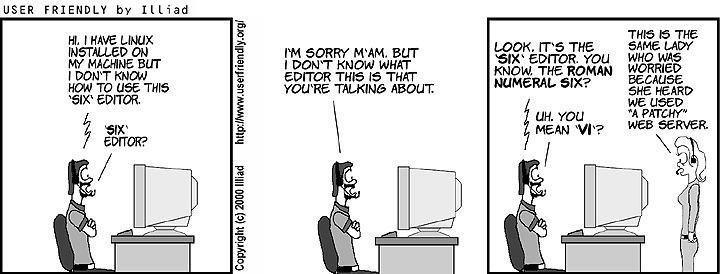
\includegraphics[scale=0.5]{images/uf001688}
  \end{center}
  \caption{Van:userfriend.org}
  \label{fig:setup}
\end{figure}

\section{Emacs}
Omdat er ook mensen waren die met een \emph{handige} \emph{editor} wilden werken, is er ook \'{e}\'{e}n onstaan met de naam \texttt{emacs}\index{index}. Deze \emph{editor} is nog modulairder dan \texttt{vim}\index{vim} en is volgens velen ook handiger in gebruik, al is dit een gegarandeerd discussiepunt. In bijlage \ref{app.emacs} is een kleine inleiding tot het gebruik van \texttt{emacs}\index{emacs} te vinden. 

\begin{figure}[H]
  \begin{center}
    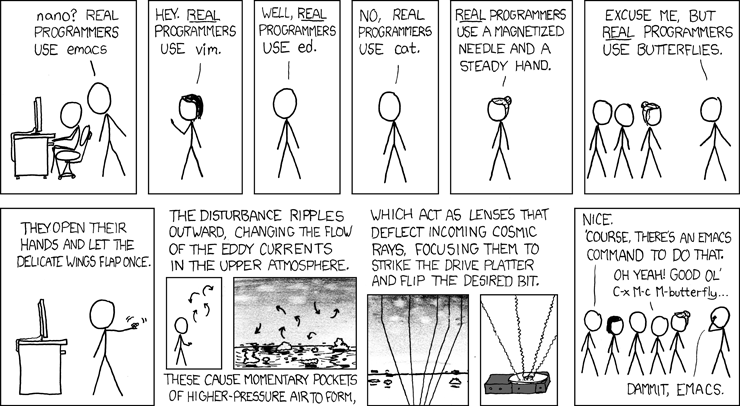
\includegraphics[scale=0.5]{images/real_programmers}
  \end{center}
  \caption{Van:xkcd.org}
  \label{fig:XKCD_emacs_butterfly}
\end{figure}

% tirlnx01 - Materiaal om het keuzevak Linux te geven 
% op de Hogeschool Rotterdam.
% Copyright (C) 2010 - 2011  Paul Sohier, Kevin van der Vlist
%
% This program is free software: you can redistribute it and/or modify
% it under the terms of the GNU General Public License as published by
% the Free Software Foundation, either version 3 of the License, or
% (at your option) any later version.
%
% This program is distributed in the hope that it will be useful,
% but WITHOUT ANY WARRANTY; without even the implied warranty of
% MERCHANTABILITY or FITNESS FOR A PARTICULAR PURPOSE.  See the
% GNU General Public License for more details.
%
% You should have received a copy of the GNU General Public License
% along with this program.  If not, see <http://www.gnu.org/licenses/>.
%
% Kevin van der Vlist - kevin@kevinvandervlist.nl
% Paul Sohier - paul@paulsohier.nl

\chapter{User management}\index{user management}
\emph{Linux} biedt uitgebreide mogelijkheden tot \emph{user management}. Omdat de dingen die in dit hoofdstuk worden uitgelegd voor meer \emph{Unices} gelden, zal het kennis zijn die altijd van pas zal komen. Wanneer de uitleg als kort wordt ervaren kan er door de lezer altijd worden teruggegrepen op de \texttt{man}\index{man} pages van het betreffende onderwerp. 

\section{Commando's}
Het is natuurlijk erg handig om de mogelijkheid te hebben om te kijken wie er momenteel op een systeem bezig is, of wie er ingelogd is geweest. Het zien, en eventueel veranderen van gebruikersinformatie behoord ook tot de mogelijkheden. 

\subsection{who}\index{who}
\texttt{who}\index{who} is een commando dat laat zien welke gebruikers er momenteel zijn ingelogd. Ook is te zien welke terminal ze gebruiken en wanneer ze zijn ingelogd: 
\begin{lstlisting}
kevin@slackbak:~$ who
kevin    pts/0        2010-12-08 08:47 (145.24.213.121)
paul     pts/1        2010-12-08 09:09 (145.24.213.56)
\end{lstlisting}%$

\subsection{w}\index{w}
Het commando \texttt{w}\index{w} laat zien wie er is ingelogd en welke taak ze momenteel uitvoeren. Ook wordt de huidige \emph{load} van het systeem geprint: 
\begin{lstlisting}
kevin@slackbak:~$ w
 09:10:13 up 19:21,  2 users,  load average: 0.00, 0.00, 0.00
USER  TTY   FROM           LOGIN@ IDLE  JCPU  PCPU WHAT
kevin pts/0 145.24.213.121 08:47  0.00s 0.02s 0.00s w
paul  pts/1 145.24.213.56  09:09  4.00s 0.04s 0.03s emacs
\end{lstlisting}%$

\subsection{last}\index{last}
\texttt{last}\index{last} kan gebruikt worden om te zien welke gebruikers er wanneer hebben ingelogd in het systeem: 
\begin{lstlisting}
kevin@slackbak:~$ last
paul  pts/1 145.24.213.56  Thu Dec 9 13:01 - 17:42 (04:40)    
kevin pts/0 145.24.213.121 Thu Dec 9 12:52 - 13:06 (00:13)    
kevin pts/0 145.24.213.121 Thu Dec 9 12:49 - 12:51 (00:02) 
\end{lstlisting}%$

\subsection{getent}\index{getent}
Het commando \texttt{getent}\index{getent} wordt gebruikt om \emph{entries} uit administratieve databases te laten zien. Er kan dus gebruikersinformatie opgehaald worden. Welke databases er worden gebruikt hangt af van de configuratie van het systeem. Standaard zullen dit waarschijnlijk de bestanden \emph{/etc/passwd} en \emph{/etc/group} zijn voor gebruikers en groeps informatie. 

Om de informatie van een gebruiker met de naam ``kevin'' te laten zien kan er het volgende gedaan worden: 
\begin{lstlisting}
kevin@slackbak:~$ getent passwd kevin
kevin:x:1000:100:Kevin van der Vlist,,,:/home/kevin:/bin/bash
\end{lstlisting}%$

\subsection{usermod}\index{usermod}
\texttt{usermod}\index{usermod} stelt een beheerder in staat om gebruikersinformatie aan te passen. Het onderstaande commando laat zien hoe de gebruiker ``kevin'' word toegevoegd aan de groep ``wheel'': 
\begin{lstlisting}
usermod -a -G wheel kevin
\end{lstlisting}

\subsection{chown}\index{chown}
Het commando \texttt{chown}\index{chown} stelt een gebruiker in staat om de eigenaar van een bestand te veranderen. Dit kan natuurlijk alleen als de gebruiker voldoende rechten heeft voor de beoogde wijziging. Het is als ``root'' gebruiker altijd mogelijk om dit commando uit te voeren. 
\begin{lstlisting}
kevin@slackbak:~$ getent group projectgroep
projectgroep:x:1001:kevin,paul
kevin@slackbak:~$ mkdir map
kevin@slackbak:~$ chmod 750 map
kevin@slackbak:~$ ls -l
total 4
drwxrwx--- 2 kevin users 4096 Dec  8 10:45 map
kevin@slackbak:~$ chown kevin:projectgroep map/
kevin@slackbak:~$ ls -l
total 4
drwxrwx--- 2 kevin projectgroep 4096 2010-12-08 10:45 map/
\end{lstlisting}
Hier is te zien dat er een nieuwe map wordt aangemaakt waar de gebruikers ``paul'' en ``kevin'' in kunnen werken. Op deze manier kan er dus op een veilige manier informatie gedeeld worden. Een gebruiker buiten \emph{projectgroep} kan immers niet de map in. 

\section{User Identifiers}\index{uid}
Een \emph{user identifier}, of \emph{uid}, is een uniek getal dat een gebruiker op een \emph{Linux} systeem toegewezen krijgt. Dit getal wordt gebruikt om een gebruiker te identificeren, bijvoorbeeld als eigenaar van een bestand. Er kunnen dus geen twee gebruikers met hetzelfde \emph{uid} voorkomen. 

De ``root'' gebruiker is een speciale gebruiker. Deze krijgt het \emph{uid} 0. Wanneer er in de \emph{source code} van de \emph{Linux kernel} wordt gekeken zal er ook zichtbaar zijn dat er bij belangrijke operaties wordt gekeken of het \emph{uid} van de actieve user 0 is. Er wordt hier wel onderscheid gemaakt tussen een \emph{real user id} en een \emph{effective user id}. 

\subsection{Real User ID}\index{real uid}
Het \emph{real uid} is het echte \emph{uid} van een gebruiker. Dit is het nummer wat te zien is wanneer de gebruikers informatie wordt opgevraagd. Dit is dus het nummer dat ook wordt gebruikt om bestanden aan de gebruiker te koppelen. 

\subsection{Effective User ID}\index{effective uid}
Het \emph{effective uid} is nagenoeg altijd hetzelfde als het \emph{real uid}. Wanneer het \emph{sticky bit} is ingesteld op een bepaald commando zal er pas iets veranderen. De gebruiker behoud dan zijn \emph{real uid}, maar veranderd zijn \emph{effective uid} naar het uid van de \emph{eigenaar} van het bestand. Laten we dit illustreren met een voorbeeld:
\begin{lstlisting}
kevin@slackbak:~$ ls -ln /usr/bin/passwd
-rws--x--x 1 0 0 56255 Feb 28  2010 /usr/bin/passwd
\end{lstlisting}%$
Hier is te zien dat het passwd commando van de gebruiker met uid 0 is, dus van ``root''. We zien echter ook dat het \emph{set-uid} bit is aangezet\footnote{Dit is aangegeven met de s in de chmod waarde, zie \texttt{man chmod} voor meer informatie.}. Wanneer we dit als gebruiker uitvoeren zal tijdens het commando het volgende gelden:
\begin{tabular}[t]{ll}
  \hline
  Wat & Waarde\\
  \hline
  Real UID & 1000\\
  Effective UID & 0\\
\end{tabular}\\
Dit zorgt ervoor dat het programma toegang krijgt tot bestanden die eigenlijk alleen voor de ``root'' gebruiker beschikbaar zijn. 

\section{File mode bits}\index{file mode bits}
\emph{File mode bits} worden gebruikt om bij te houden of gebruikers rechten hebben om een bepaalde file of map te openen of te beschrijven. Deze rechten worden per bestand of map opgeslagen. Het manifesteert zich als volgt:
\begin{lstlisting}
kevin@slackbak:~$ ls -l /home/
total 28
drwxr-xr-x 2 root  root   4096 Feb 13  2010 ftp
drwxr-x--x 3 kevin users  4096 Dec  8 09:39 kevin
drwx------ 2 root  root  16384 Dec  6 13:25 lost+found
drwx--x--x 2 paul  users  4096 Dec  8 09:10 paul
-rw-r--r-- 1 kevin users 0 Dec  8 09:58 bestand
\end{lstlisting}%$
De eerste kolom is de belangrijkste in dit geval. Als voorbeeld wordt er naar de map \emph{kevin} gekeken:
\begin{lstlisting}
drwxr-x--x
\end{lstlisting}
De eerste letter, de \emph{d}, kan verschillende waardes hebben. Elke waarde staat voor een aparte categorie. Deze zijn als volgt:

\begin{tabular}[t]{lll}
  \hline
  Wat & Betekenis\\
  \hline
  - & file\\
  d & directory\\
  b & block special file\\
  c & character special file\\
  l & symbolic link\\
  p & named pipe\\
  s & domain socket\\
\end{tabular}\\
Hierna word er naar groepen van 3 karakters gekeken. De eerste kolom staat voor de rechten van de eigenaar, de tweede groep staat voor de rechten van de groep en de derde staat voor de rechten voor world, de rest. De \emph{r} staat voor read, \emph{w} staat voor write en \emph{x} betekend execute. 
Wanneer we de bovenstaande rechten erbij pakken, zien we het volgende:

\begin{tabular}[t]{lll}
  \hline
  Wie & Rechten & Betekenis\\
  \hline
  owner & rwx & Lezen, schrijven en uitvoeren.\\
  group & r-x & Lezen en uitvoeren.\\
  other & \-\-x & Uitvoeren.\\
\end{tabular}

Aangezien het hier een map betreft heeft \emph{uitvoeren} een speciale betekenis, namelijk de rechten om een map te openen. Het is belangrijk om hier rekening mee te houden:
\begin{lstlisting}
kevin@slackbak:~$ mkdir map
kevin@slackbak:~$ touch map/file
kevin@slackbak:~$ ls -lhR map/
map/:
total 0
-rw-r--r-- 1 kevin users 0 Dec  8 10:30 file
kevin@slackbak:~$ chmod 600 map/
kevin@slackbak:~$ ls -lhR map/
map/:
ls: cannot access map/file: Permission denied
total 0
-????????? ? ? ? ?            ? file
\end{lstlisting}%$
Zoals hierboven te zien is, kan het ``gekke'' resultaten opleveren wanneer een bestand genoeg rechten heeft, maar de map waar deze in staat niet. 

Voor normale bestanden betekend de \emph{uitvoeren} optie dat het bestand uitgevoerd mag worden als shell script. Wanneer dit niet ingesteld is, zal je een \emph{permission denied} foutmelding krijgen op het bestand: 
\begin{lstlisting}
paul@slackbak:~$ ls -l
total 0
-rw-r--r-- 1 paul users 0 2010-12-15 23:37 test.sh
paul@slackbak:~$ ./test.sh
-bash: ./test.sh: Permission denied
\end{lstlisting} 
Ook als er gebruik gemaakt wordt van een taal zoals bijvoorbeeld \emph{perl}, \emph{python} of \emph{php} moet je de permissies op \emph{execute} zetten het bestand te draaien.\index{perl}\index{python}\index{php}

\subsection{Waardes}
De volgende waardes worden gebruikt om rechten aan te geven:\\
\begin{tabular}[t]{lll}
  \hline
  waarde & binair & betekenis\\
  \hline
  1 & 001 & Uitvoeren\\
  2 & 010 & Schrijven\\
  4 & 100 & Lezen\\
\end{tabular}

Deze waardes worden in de praktijk gebruikt voor \texttt{chmod}\index{chmod}
\begin{lstlisting}
kevin@slackbak:~$ chmod 600 map
\end{lstlisting}%$
Dit commando stelt voor de categorie \emph{user} de rechten op 6, binair \emph{110}. Dit betekend dus lezen, schrijven en niet uitvoeren. De rest staat op 0, dus geen toegang. 

\subsection{Gebruik van numerieke waarden}
In veel voorbeelden, zowel in dit document als buiten dit document, zal er gebruikt gemaakt worden van de numerieke varianten, in plaats van de letters. Het is dus belangrijk dat je weet wat de verschillende numerieke waarden betekenen. 

\subsection{umask}
Om te kunnen be\"{i}nvloeden onder welke rechten een bestand word aangemaakt door een proces kan er gebruik gemaakt worden van een \texttt{umask}\index{umask}. Dit staat voor \textbf{u}ser \textbf{mask}. Het betekend dat een proces bepaalde bits gekoppeld aan de file mode bits weghaald. Dit word met een bitwise operatie gedaan, bijvoorbeeld \texttt{777 \& (\~{}022) = 755}. Dit is gemakkelijker te zien met een klein voorbeeld:
\begin{lstlisting}
kevin@slackbak /tmp/demo$ umask 755
kevin@slackbak /tmp/demo$ touch file
kevin@slackbak /tmp/demo$ umask 177
kevin@slackbak /tmp/demo$ touch prive
kevin@slackbak /tmp/demo$ umask 133
kevin@slackbak /tmp/demo$ touch hoi
kevin@slackbak /tmp/demo$ umask 100
kevin@slackbak /tmp/demo$ touch dag
kevin@slackbak /tmp/demo$ ls -lh
total 0
-rw-rw-rw- 1 kevin users 0 2011-04-13 10:24 dag
-----w--w- 1 kevin users 0 2011-04-13 10:24 file
-rw-r--r-- 1 kevin users 0 2011-04-13 10:24 hoi
-rw------- 1 kevin users 0 2011-04-13 10:24 prive
\end{lstlisting}%$

Hier is te zien dat een \texttt{umask}\index{umask} van \texttt{755} resulteert in het weghalen van alle rechten, behalve \emph{read} (octaal 2). Wanneer het \texttt{umask}\index{umask} vervolgens word veranderd naar iets heel anders, bijvoorbeeld 100, blijkt dat er lees en schrijf rechten overblijven.

% tirlnx01 - Materiaal om het keuzevak Linux te geven 
% op de Hogeschool Rotterdam.
% Copyright (C) 2010 - 2011  Paul Sohier, Kevin van der Vlist
%
% This program is free software: you can redistribute it and/or modify
% it under the terms of the GNU General Public License as published by
% the Free Software Foundation, either version 3 of the License, or
% (at your option) any later version.
%
% This program is distributed in the hope that it will be useful,
% but WITHOUT ANY WARRANTY; without even the implied warranty of
% MERCHANTABILITY or FITNESS FOR A PARTICULAR PURPOSE.  See the
% GNU General Public License for more details.
%
% You should have received a copy of the GNU General Public License
% along with this program.  If not, see <http://www.gnu.org/licenses/>.
%
% Kevin van der Vlist - kevin@kevinvandervlist.nl
% Paul Sohier - paul@paulsohier.nl

\chapter{Proces management}
Een \emph{proces} is een actief programma op een machine. Onder actief wordt verstaan dat het programma een gedeelte van de \emph{systeem resources} wil gebruiken. Hiervoor zal het echter wel van de \emph{kernel} toegang moeten krijgen. 

\section{Processen bekijken}
Er zijn verschillende manier om te zien welke \emph{processen} er actief zijn. De meest gebruikte varianten zijn \texttt{ps}\index{ps} en \texttt{top}\index{top}. 
\begin{lstlisting}
kevin@slackbak:~$ man ps
[...]
-e              Select all processes. Identical to -A.
-f              does full-format listing. [...]
kevin@slackbak:~$ ps -ef 
UID   PID PPID  C STIME TTY   TIME     CMD
root  1   0     0 Dec07 ?     00:00:02 init [3]  
root  2   0     0 Dec07 ?     00:00:00 [kthreadd]
[...]
root  2227 1406 0 10:48 ?     00:00:00 sshd: kevin [priv]
kevin 2229 2227 0 10:48 ?     00:00:00 sshd: kevin@pts/0
kevin 2230 2229 0 10:48 pts/0 00:00:00 -bash
kevin 2280 2230 0 11:08 pts/0 00:00:00 ps -ef
\end{lstlisting}
Wanneer deze listing begrepen wordt is er veel informatie uit te halen. Aangezien dit belangrijke en handige informatie betreft, zullen alle kolommen de nodige uitleg krijgen. 

\subsection{UID}
Deze kolom bevat het \emph{effective uid} van het proces op de betreffende regel. Hier blijkt dus onder welke gebruiker een \emph{proces} effectief draait. 

\subsection{PID}\index{pid}
In deze kolom is het \emph{proces id}, of \emph{pid} te zien. Dit \emph{proces id} is een unieke identifier van een \emph{proces}, en kan daarom slechts eenmalig voorkomen. Dit \emph{pid} word gebruikt wanneer een bepaald proces moet worden gespecificeerd.

\subsection{PPID}\index{parent pid}
Dit is het \emph{parent proces id} van een \emph{proces}. Dit geeft het \emph{pid} weer van het proces wat (meestal met behulp van \emph{fork()} een \emph{child} proces heeft gestart. De relatie van een \emph{proces} met zijn parent is een heel belangrijke. Een proces kan namelijk niet leven zonder \emph{parent}. Als de parent sterft, zal het child proces ook mee gaan, tenzij deze is \emph{detached}. 

\subsection{C}
Dit is de integer representatie van het cpu gebruik. Het cijfer wordt als volgt berekend:
$$ \frac{cputijd}{echte\_tijd} \cdot 100 = (int) bezetting$$
\emph{cputijd} is hierbij de tijd waarin een proces zich in \emph{running state} bevindt, \emph{echte\_tijd} is de echte tijd. Het proces om deze \emph{PDF} te maken heeft de volgende kenmerken:
\begin{lstlisting}
real    0m15.877s
user    0m8.221s
\end{lstlisting}
\emph{Cputijd} zou hier dus zijn:
$$ \frac{8.221}{15.877} \cdot 100 = 51.7793034$$
$$(int) bezetting = 51$$

\subsection{STIME}
De kolom \emph{STIME} bevat de start time van het \emph{proces}. 

\subsection{TTY}
In de kolom \emph{TTY} staat de \emph{terminal} waar het proces draait. 

\subsection{TIME}
Dit is de hoeveelheid \emph{cputijd} die een proces heeft gebruikt. Hoe hoger \emph{TIME} is, hoe actiever een \emph{proces} dus is. 

\subsection{CMD}
In deze laatste kolom is de naam van het \emph{proces} te zien, samen met de betreffende parameters. 

\section{Termination} 
Wanneer een \emph{proces} niet meer reageert, of taken gaat uitvoeren die niet binnen zijn takenpakket vallen, kan het zijn dat een proces afgeschoten moet worden. Het commando \texttt{kill}\index{kill} biedt deze mogelijkheid, door een \emph{signal} naar het proces te sturen. Deze \emph{signals} zijn onderdeel van de \emph{POSIX} standaard. De twee belangrijkste signals voor nu zijn \emph{SIGTERM} en \emph{SIGKILL}. Om te kijken wat dit precies betekend zou je in \texttt{man 7 signal} kunnen kijken.

Het eerste \emph{signal} geeft een proces te kennen dat het be\"{i}ndigd moet worden. Het proces zal dan afsluiten: 
\begin{lstlisting}
kevin@slackbak:~$ sleep 10&
[1] 2427
kevin@slackbak:~$ kill 2427
kevin@slackbak:~$ ps -ef | grep sleep
kevin     2429  2230  0 12:28 pts/0    00:00:00 grep sleep
[1]+  Terminated              sleep 10
\end{lstlisting}%$
Een \emph{proces} kan een \emph{SIGTERM} signal afvangen en negeren. Een andere mogelijkheid is dat een \emph{proces} ongedefinieerd gedrag gaat vertonen. Beide situaties kunnen resulteren in een proces dat niet is te stoppen door een \emph{SIGTERM} te sturen: 
\begin{lstlisting}
kevin@slackbak:~$ top&
[1] 2430
kevin@slackbak:~$ kill 2430
[1]+  Stopped                 top
kevin@slackbak:~$ ps -ef | grep top
kevin     2430  2230  0 12:28 pts/0    00:00:00 top
kevin     2434  2230  0 12:29 pts/0    00:00:00 grep top
kevin@slackbak:~$ kill -9 2430
kevin@slackbak:~$ ps -ef | grep top
kevin     2436  2230  0 12:29 pts/0    00:00:00 grep top
[1]+  Killed                  top
\end{lstlisting}%$
Het \emph{SIGHUP} \emph{signal} kan ook door programmeurs worden afgevangen. Dit signal wordt veel gebruikt om een \emph{proces} te laten herstarten. De werking is weer hetzelfde. 
\begin{lstlisting}
kevin@slackbak:~$ kill -HUP 1337
\end{lstlisting}%$
Na het uitvoeren van het \texttt{kill}\index{kill} commando met \emph{PID} 1337 als parameter, zal het \emph{proces} met 1337 als \emph{PID} herstarten zonder dat deze afsluit. 

\section{Zombies}\index{zombie}
\emph{Zombie processen} zijn een speciaal soort processen. Deze processen zijn klaar met het uitvoeren van hun taken en zouden dus moeten verdwijnen uit de \emph{process table}. De \emph{parent} van een \emph{proces} heeft echter nog de mogelijkheid om de exit status van een \emph{child proces} te bekijken. Wanneer dit niet gebeurd, zal het proces nog aanwezig blijven in de \emph{process table}. \emph{Zombie's} zijn per definitie \emph{processen} die geen \emph{resources} gebruiken, dus de enige 'last' die een gebruiker ervan ondervindt is de entry in de \emph{process table}. 

Een \emph{zombie proces} afschieten is niet altijd mogelijk. Wanneer een \emph{zombie proces} een \emph{parent pid} heeft, is het mogelijk om de \emph{parent} af te sluiten. \emph{Childs} zullen hierdoor ook sterven, waardoor de \emph{zombie} weg is. 

Wanneer een \emph{zombie} \texttt{init}\index{init} (pid 1) als \emph{parent} heeft, zal het onmogelijk zijn het \emph{proces} af te sluiten. De enige manier om de \emph{zombie} dan weg te krijgen is een complete reboot. 

\section{Load}
\emph{Load}\cite{bib.load} is een belangrijk getal in de \emph{Linux} wereld. De getallen bij \emph{load} geven aan hoe druk de \emph{CPU} is, maar het interpreteren van het getal gebeurd vaak fout.

De \emph{load} kan via diverse commando's opgevraagd worden, te weten:
\begin{itemize}
  \item \texttt{uptime}\index{uptime}
  \item \texttt{w}\index{w}
  \item \texttt{top}\index{top}
  \item De file \emph{/proc/loadavg}\index{/proc/loadavg}
\end{itemize}
Alle commando's zullen (In principe) dezelfde waarde teruggeven als resultaat.

Bij een computer die niets zal te doen zal de \emph{load} 0.00 zijn.\footnote{\emph{UNIX} en \emph{Linux} verschillen in het berekenen van de \emph{load}. \emph{UNIX} gebruikt alleen de processen welke in \emph{RUNNING} of \emph{RUNNABLE} state zijn, terwijl \emph{Linux} ook de processen in de \emph{uninterruptible} state meerekent. }
Wanneer je het commando \texttt{load} uitvoert komen er drie cijfers uit: 
\begin{lstlisting}
paul@slackbak:~$ uptime  
 16:47:37 up 6 days, 17:37,  1 user,  load average: 0.00, 0.00, 0.00
\end{lstlisting}%$
Zoals te zien heeft onze server momenteel niets te doen.

\begin{lstlisting}
srv01:~# uptime 
 17:05:30 up 224 days,  3:01,  1 user,  load average: 2.37, 3.42, 0.39
\end{lstlisting}
Deze server heeft het een stuk drukker. De drie waardes geven de \emph{load} aan van de laatste minuut, vijf minuten en vijftien minuten. In het geval van hierboven staat er:\footnote{Let op: Dit voorbeeld gaat uit van \'{e}\'{e}n \emph{CPU core}. Wanneer er meer als \'{e}\'{e}n core is, dan moet er in plaats van \'{e}\'{e}n het aantal cores van de load afgehaald worden.}
\begin{itemize}
  \item In de laatste minuut was de \emph{CPU} overbelast met \emph{137\%}.
  \item In de laatste vijf minuten was de \emph{CPU} overbelast met \emph{242\%}.
  \item In de laatste vijftien minuten was de \emph{CPU} onderbelast met \emph{61\%}.
\end{itemize}
Wanneer de \emph{CPU} 1,37 keer sneller was geweest als de huidige \emph{CPU} dan had de \emph{CPU} alle taken in die minuut kunnen uitvoeren.
Een \emph{load} van precies 1.00 betekend dat de \emph{CPU}, indien er \'{e}\'{e}n core is, volledig gebruikt wordt voor die minuut. Als je bijvoorbeeld 4 cores ter berschikking hebt en een \emph{load} van 4.00, betekend dit hetzelfde als een \emph{load} van 1.00 bij een enkele core.

% tirlnx01 - Materiaal om het keuzevak Linux te geven 
% op de Hogeschool Rotterdam.
% Copyright (C) 2010 - 2011  Paul Sohier, Kevin van der Vlist
%
% This program is free software: you can redistribute it and/or modify
% it under the terms of the GNU General Public License as published by
% the Free Software Foundation, either version 3 of the License, or
% (at your option) any later version.
%
% This program is distributed in the hope that it will be useful,
% but WITHOUT ANY WARRANTY; without even the implied warranty of
% MERCHANTABILITY or FITNESS FOR A PARTICULAR PURPOSE.  See the
% GNU General Public License for more details.
%
% You should have received a copy of the GNU General Public License
% along with this program.  If not, see <http://www.gnu.org/licenses/>.
%
% Kevin van der Vlist - kevin@kevinvandervlist.nl
% Paul Sohier - paul@paulsohier.nl

\chapter{Linux networking}\label{h.netwerk}
\emph{Linux} is enorm geschikt om te gebruiken in netwerk gerelateerde toepassingen. Doordat het een \emph{multi-user} systeem is, is het erg gemakkelijk om gebruikers via het netwerk diensten aan te bieden. Voordat een systeem bereikbaar is moet er natuurlijk wel een netwerk configuratie gedaan worden. Daarna willen we een paar veel gebruikte services aanduiden. 

\section{Configuratie}
Het netwerk kan op twee manieren worden ingesteld. Er kan gekozen worden om een automatische configuratie te doen, maar er kan ook voor de handmatige manier gekozen worden. We zullen beide manieren beschrijven. 

\subsection{netconfig}
Om het netwerk in te stellen is er een script wat je hierbij helpt. Dit script heet \texttt{netconfig}. De werking hiervan is enorm eenvouding. Er worden per stap wat vragen aan je gesteld. Geef antwoord op de vragen, en bevestig daarna je instellingen. \texttt{netconfig} zal ze dan toepassen.
\begin{lstlisting}
root@slackbak:/home/kevin# netconfig
\end{lstlisting}\index{netconfig}

\subsection{Handmatige configuratie}\index{rc.inet1.conf}
Om het netwerk handmatig te configureren is het nodig om de netwerk config file aan te passen. Dit bestand bevat alle netwerk gerelateerde configuratie. We zullen hier de relevante informatie geven van een bedraad device onder de naam \emph{eth0}.
\begin{lstlisting}
root@slackbak:/home/kevin# cat /etc/rc.d/rc.inet1.conf 
[...]
# If USE_DHCP[interface] is set to "yes"
# this overrides any other settings.
IPADDR[0]="145.24.222.162"
NETMASK[0]="255.255.255.0"
USE_DHCP[0]=""
DHCP_HOSTNAME[0]=""
[...]
# Default gateway IP address:
GATEWAY="145.24.222.253"
[...]
kevin@slackbak:~$ cat /etc/HOSTNAME 
slackbak.cmi-hro.nl
\end{lstlisting}%$
\index{cat}\index{/etc/HOSTNAME}
Zoals je kunt zien is er niets wereld schokkends aan de config file. Alle velden spreken voorzich. Wanneer het systeem up komt, zullen bovenstaande waardes uitgelezen worden waarna het systeem ze zal gebruiken. 

\subsection{/etc/hosts}\index{/etc/hosts}
Deze file bevat verwijzingen naar hosts op het netwerk, welke niet door de \emph{DNS} server gegeven zullen worden opgezocht. De syntax vereist geen uitleg:
\begin{lstlisting}
127.0.0.1               localhost
145.24.222.162          slackbak.cmi-hro.nl slackbak
145.24.129.221          ftphro.nl ftphro
\end{lstlisting}

\subsection{/etc/resolv.conf}\index{/etc/resolv.conf}
Om de \emph{DNS} in te stellen kan de file \texttt{/etc/resolv.conf} gebruikt worden. DNS servers toevoegen gaat erg gemakkelijk:
\begin{lstlisting}
root@slackbak:/home/kevin# cat /etc/resolv.conf 
nameserver 145.24.129.1
nameserver 145.24.129.2
\end{lstlisting}

\subsection{ifconfig}\index{ifconfig}
Om netwerk instellingen te doen zonder config files aan te passen en services te reloaden is er ook een tool genaamd \texttt{ifconfig} beschikbaar. De output hiervan is behoorlijk intimiderend. Wanneer er echter rustig naar gekeken word, vallen veel regels al op zijn plaats. Wanneer de velden niet duidelijk zijn verwijzen we weer door naar de \emph{man pages}. 
\begin{lstlisting}
kevin@slackbak:~$ /sbin/ifconfig 
eth0 Link encap:Ethernet  HWaddr 00:0c:29:fa:16:57  
     inet addr:145.24.222.162 Bcast:145.24.222.255 Mask:255.255.255.0
     inet6 addr: fe80::20c:29ff:fefa:1657/64 Scope:Link
     UP BROADCAST RUNNING MULTICAST  MTU:1500  Metric:1
     RX packets:16340 errors:0 dropped:0 overruns:0 frame:0
     TX packets:5796 errors:0 dropped:0 overruns:0 carrier:0
     collisions:0 txqueuelen:1000 
     RX bytes:1858849 (1.7 MiB)  TX bytes:1138260 (1.0 MiB)
     Interrupt:18 Base address:0x1400 

lo   Link encap:Local Loopback  
     inet addr:127.0.0.1  Mask:255.0.0.0
     inet6 addr: ::1/128 Scope:Host
     UP LOOPBACK RUNNING  MTU:16436  Metric:1
     RX packets:0 errors:0 dropped:0 overruns:0 frame:0
     TX packets:0 errors:0 dropped:0 overruns:0 carrier:0
     collisions:0 txqueuelen:0 
     RX bytes:0 (0.0 B)  TX bytes:0 (0.0 B)
\end{lstlisting}%$
Deze uitvoer laat de instellingen van twee netwerk devices zien. Namelijk \emph{eth0} en \emph{lo}. Dit zijn respectievelijk de netwerk-kaart en het loopback device. De netwerkkaart (nic) is ingesteld met het commando \texttt{netconfig} en het loopback device (lo) is altijd aanwezig, ook al is er geen nic aanwezig is. 
\begin{lstlisting}
root@slackbak:/home/kevin# ifconfig eth0 down
\end{lstlisting}
Met het commando \texttt{ifconfig} kunnen de network devices ingesteld en verwijderd worden. De manual page van \texttt{ifconfig} zegt dat de synopsis van \texttt{ifconfig}: 'ifconfig interface options' is. Het commando \texttt{ifconfig eth0 down} zorgt ervoor dat de device eth0 verwijderd wordt uit de network configuratie.

\section{SSH}
\subsection{Het verleden}\index{telnet}
Om via het netwerk op een andere machine te werken kan er gebruik gemaakt worden van een remote terminal. De software die een remote terminal mogelijk maakt is in feite niets meer dan een virtueel toetsenbord en een virtuele output device. In het verleden werd hier \emph{telnet} voor gebruikt. 

Een van de grootste nadelen van \emph{telnet} is het gemak waar de communicatie mee afgeluisterd kan worden. Telnet verstuurt al zijn verkeer namelijk onversleuteld. Wanneer je via telnet afgeluisterd zou worden, word dus ook het ``root'' wachtwoord van de betreffende server gecompromitteerd. Omdat servers vaak grote hoeveelheden gevoelige data bevatten is dit een groot gevaar voor de integriteit van onze moderne digitale infrastructuur. 

\subsection{OpenSSH}\index{ssh}
Om toch veilig te kunnen werken op machines waar je via het netwerk mee verbonden bent is er een programma ontwikkeld wat bekend staat onder de naam \emph{openssh}. Deze naam staat voor 'open secure shell', een techniek die van oorsprong uit de \emph{BSD} wereld komt. Deze techniek is dankzij het open karakter van de \emph{BSD-style} licenties uitgegroeid tot een industrie standaard voor remote terminals. 

\emph{OpenSSH} bestaat uit twee delen, een server en een client. De server luisterd standaard op poort 22 naar inkomende verbindingen geiniti\"{e}erd door de OpenSSH client. Omdat SSH een fundamenteel onderdeel is voor onderlinge communicatie tussen servers, maar ook voor onderhoud zullen we in appendix \ref{app.ssh} een overzicht geven over de werking van SSH. 

\subsection{De eerste keer}
Wanneer er voor het eerst verbinding word gemaakt met een host zal het volgende te zien zijn.
\begin{lstlisting}
kevin@slackbak:~$ scp kevin@host.nl:/home/kevin/backup.tar.gz ~/backup.gz
The authenticity of host 'host.nl (1.2.3.4)' can't be established.
RSA key fingerprint is 0e:35:8e:be:6a:61:f0:dd:b1:ef:fe:a6:7f:f6:a5:da.
Are you sure you want to continue connecting (yes/no)? yes
Warning: Permanently added 'host.nl,1.2.3.4' (RSA) to the list of known hosts.
kevin@host.nl's password:
\end{lstlisting}%$
Hiermee wordt de identiteit van een host gecontroleerd. In de toekomst zal dit gebruikt worden om te verifi\"{e}ren of er weer met dezelfde host verbinding wordt gemaakt. 

Het is dus belangrijk om te zorgen dat de \emph{RSA key fingerprint} correct is. Dit is te controleren door deze handmatig te vergelijken met de fingerprint van de server. Vraag bij de beheerder de key op, of controleer hem zelf na de configuratie van server:
\begin{lstlisting}
kevin@slackbak:~$ ssh-keygen -l -f /etc/ssh/ssh_host_rsa_key
2048 0e:35:8e:be:6a:61:f0:dd:b1:ef:fe:a6:7f:f6:a5:da /etc/ssh/ssh_host_rsa_key.pub (RSA)
\end{lstlisting}%$

\subsection{Verbinding}
Wanneer een gebruiker succesvol is ingelogd via SSH, kan er gemakkelijk op het remote systeem gewerkt worden. Alle commando's die in de shell worden uitgevoerd zullen op de remote host gedraaid worden. Het is net alsof je fysiek achter de computer zit. 

\subsection{Problemen}
Wanner de unieke host key van een host is gewijzigd betekend dit dat de unieke fingerprint is gewijzigd. Dit kan zo bedoeld zijn, bijvoorbeeld door een nieuwe installatie waarbij nieuwe keys gegenereerd zijn. Wanneer dit niet zo is zijn we bij optie twee aangekomen; iemand is met de verbinding aan het rotzooien. Let dus enorm op bij de volgende scherm:
\begin{lstlisting}
kevin@slackbak:~$ ssh kevin@host.nl
@@@@@@@@@@@@@@@@@@@@@@@@@@@@@@@@@@@@@@@@@@@@@@@@@@@@@@@@@@@
@    WARNING: REMOTE HOST IDENTIFICATION HAS CHANGED!     @
@@@@@@@@@@@@@@@@@@@@@@@@@@@@@@@@@@@@@@@@@@@@@@@@@@@@@@@@@@@
IT IS POSSIBLE THAT SOMEONE IS DOING SOMETHING NASTY!
Someone could be eavesdropping on you right now (man-in-the-middle attack)!
It is also possible that the RSA host key has just been changed.
The fingerprint for the RSA key sent by the remote host is
b4:85:5a:03:c0:07:5e:9c:52:1d:2d:54:2d:15:59:38.
Please contact your system administrator.
Add correct host key in /home/kevin/.ssh/known_hosts to get rid of this message.
Offending key in /home/kevin/.ssh/known_hosts:1
RSA host key for host.nl has changed and you have requested strict checking.
Host key verification failed.
\end{lstlisting}%$

\section{SCP}\index{scp}
Deze afkorting staat voor \emph{Secure Copy}. Dit gebruikt de faciliteiten van 
\emph{SSH} om een beveiligde verbinding op te zetten met de remote host. Over dit versleutelde kanaal kan vervolgens data verzonden worden. 
\begin{lstlisting}
kevin@slackbak:~$ scp kevin@host.nl:/home/kevin/backup.tar.gz ~/backup.gz
kevin@host.nl's password: 
backup.tar.gz 100% 10MB 88.3KB/s 01:57
\end{lstlisting}%$

\section{FTP}\index{ftp}
Een protocol wat van traditioneel veel gebruikt word om binaire data over te sturen is \emph{FTP}, het \emph{file transfer protocol}. Dit protocol is te gebruiken met het ftp commando. De meest simpele werking is als volgt.
\begin{lstlisting}
kevin@slackbak:~$ ftp ftp.hro.nl
Connected to orpheus.hro.nl.
[...]
220 Service Ready for new User
Name (ftp.hro.nl:kevin): 
\end{lstlisting}%$
of
\begin{lstlisting}
kevin@slackbak:~$ ftp
ftp> open ftp.hro.nl
Connected to orpheus.hro.nl.
[...]
220 Service Ready for new User
Name (ftp.hro.nl:kevin):
\end{lstlisting}%$
Op de regel met \emph{Name} staat 'ftp.hro.nl:kevin'. Dit betekend dat, wanneer je niets invult, er met de user kevin ingelogd zal worden. Dit word gedaan omdat dit de username op je huidige systeem is. 
Gebruik als username \emph{studentno.extensie} en als password je HRO wachtwoord. Je bent nu ingelogd op de FTP-server van de HRO.

Onthoud wel dat \emph{ftp} de data onversleuteld verstuurd. Wanneer je een verbinding dus niet vertrouwd is het af te raden om gebruik te maken van FTP. 

\section{SFTP}\index{sftp}
Omdat \emph{ftp}, zoals vermeld, gebruikt maakt van onversleutelde kanalen kan het reden zijn dit niet te gebruiken. Niemand wil natuurlijk dat zijn account gegevens van een machine op straat komen te liggen. Er kan om deze reden dan ook gebruik gemaakt worden van \emph{sftp}. Dit staat voor \emph{SSH File Transfer Protocol}, of soms het \emph{Secure File Transfer Protocol}. 

Het gebruik van \emph{sftp} lijkt erg op dat van \emph{scp}. 
\begin{lstlisting}
sftp kevin@slack.host.nl
kevin@slackbak's password: 
Connected to slack.icyx.nl.
sftp>
\end{lstlisting}
Er zijn echter wat kleine verschillen. \emph{sftp} stelt een gebruiker bijvoorbeeld ook in staat om een listing van een map op te vragen. Dit is iets wat in \emph{ftp} ook mogelijk is, maar wat met \emph{scp} niet kan zonder eerst een shell te openen. 

Een ander klein practisch voordeel boven \emph{ftp} is de mogelijkheid tot het bewaren van de originele timestamps van bestanden wanneer het word verstuurt. Voor de preciese verschillen word er zoals gewoonlijk weer naar de man page verwezen. 

% tirlnx01 - Materiaal om het keuzevak Linux te geven 
% op de Hogeschool Rotterdam.
% Copyright (C) 2010 - 2011  Paul Sohier, Kevin van der Vlist
%
% This program is free software: you can redistribute it and/or modify
% it under the terms of the GNU General Public License as published by
% the Free Software Foundation, either version 3 of the License, or
% (at your option) any later version.
%
% This program is distributed in the hope that it will be useful,
% but WITHOUT ANY WARRANTY; without even the implied warranty of
% MERCHANTABILITY or FITNESS FOR A PARTICULAR PURPOSE.  See the
% GNU General Public License for more details.
%
% You should have received a copy of the GNU General Public License
% along with this program.  If not, see <http://www.gnu.org/licenses/>.
%
% Kevin van der Vlist - kevin@kevinvandervlist.nl
% Paul Sohier - paul@paulsohier.nl

\chapter{X}
Om op een \emph{Linux} systeem gebruik te kunnen maken van een grafische omgeving is het \emph{X framework} ontwikkeld. Het is een product wat wordt geleid door de \emph{X.Org Foundation}. 

\section{Geschiedenis}
De \emph{X.Org foundation} is ontstaan uit een samenwerkingsverband tussen de organisatie die de \emph{X} standaarden regelt en een groep vroegere ontwikkelaars van het \emph{XFree86} project. 

De reden dat deze ontwikkelaars zijn overgestapt naar de \emph{X.Org foundation} is een ruzie over het nieuwe licentiemodel van \emph{XFree86}. Er heeft daarom een \emph{fork} plaatsgevonden waarna het project \emph{X11} werd ondergebracht bij de \emph{X.Org foundation}. 

\section{Implementatie}
De basis van het \emph{X} protocol is in de jaren 80 ontwikkeld. De bedoeling was om een generiek \emph{client-server} model te hebben om grafische toepassingen te gebruiken. Er moest op een willekeurige machine een applicatie gedraaid moeten worden, die gebruikt kon worden op een willekeurige andere machine. De keuze van het platform zou dit niet mogen belemmeren. 

Er zijn binnen het \emph{X} protocol twee partijen. Deze hebben allebij een eigen taak. 

\subsection{X server}
De \emph{X server} verzorgt de faciliteiten om de verschillende \emph{X clients} te kunnen laten communiceren. Ook biedt het een \emph{display} aan. Dit betekend dus dat er op een \emph{client} een \textbf{\emph{X server}} draait. 

\subsection{X client}
De \emph{X client} zal de diensten van de \emph{X server} gebruiken. De applicaties zelf zijn dus effectief de \textbf{\emph{X clients}}. Als er op een applicatie een grafisch programma wordt gestart zal dit dus een \emph{client} zijn naar de \emph{X server} van de verbonden gebruiker. 

\subsection{Protocol}
Voor de communicatie tussen de \emph{X} server en de \emph{X} client is er gekozen voor een compleet transparant protocol. Het is niet afhankelijk van het medium waar het transport over plaatsvindt, waardoor gebruikers ook via het netwerk software kunnen gebruiken. 

\subsection{Communicatie}
Wanneer alle bovenstaande aspecten bij elkaar worden gevoegd zal er het volgende totaalbeeld uit komen, zie figuur \ref{fig:xs2}:
% Plaatje niet nodig, leg in een keer 2 uit. Als het toch nodig is, hij blijft in de sources
%\begin{figure}[h]%Dit plaatje is overbodig
%  \begin{center}
%    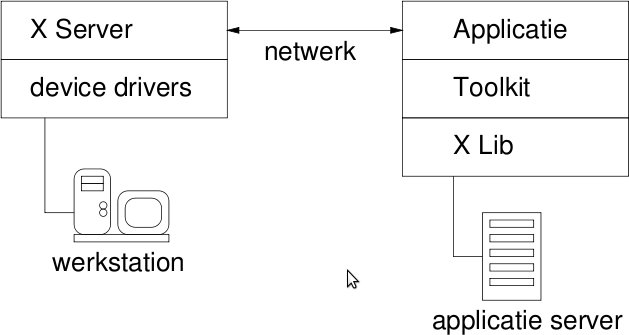
\includegraphics[scale=0.4]{images/xserver}
%  \end{center}
%  \caption{X client/server overzicht}
%  \label{fig:xs}
%\end{figure}

\begin{figure}[h]
  \begin{center}
    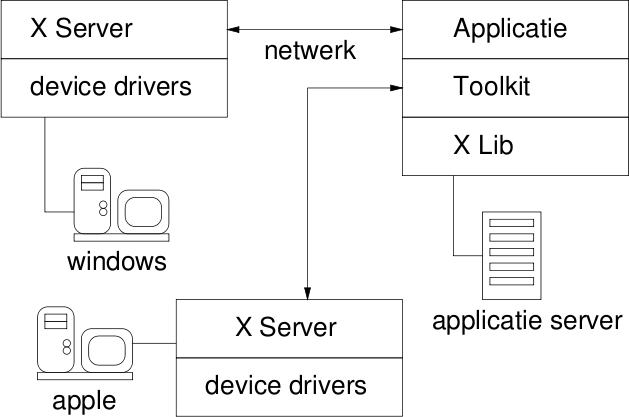
\includegraphics[scale=0.4]{images/xserver2}
  \end{center}
  \caption{X client/server overzicht}
  \label{fig:xs2}
\end{figure}
Hier is duidelijk te zien hoe de verschillende onderdelen van \emph{X} met elkaar samenwerken. Een applicatie gestart op een applicatie server is generiek. Deze zal verbinding maken met de \emph{X server} van de \emph{client}, welke de hardware-specifieke zaken regelt. Om deze reden zal de ``Apple'' computer dus een andere \emph{X server} hebben dan de ``Windows'' computer. 

\section{Window Manager}
Een \emph{window manager} is een pakket wat alle zaken regelt die gerelateerd zijn aan het venster beheer. Denk hierbij bijvoorbeeld aan de mogelijkheid om vensters te verslepen of van grootte te veranderen. De meeste \emph{window managers} zullen ook voor een \emph{desktop} omgeving zorgen, waardoor het paketten zijn die sterk zijn ge\"{i}ntegreerd met basis \emph{desktop} applicaties. 

De bekendste toepassing die een \emph{window manager} uitvoert is het \emph{reparenten} van een scherm. Hier wordt er nog een extra ``venster'' om een programma heen gezet, welke vaak bestaat uit de titelbalk. Dit kan dan bijvoorbeeld worden gebruikt om vensters te verslepen. 

\section{Installatie}
Op \emph{Slackware} zijn er ook \emph{packages} van \emph{Xorg beschikbaar}. Het installeren hiervan is dan ook relatief eenvoudig. 

Er kan gekozen worden om de volledige \emph{X} suite te installeren, of om de minimale delen ervan te kiezen. Omdat het iets gemakkelijker is om de complete \emph{X} suite te installeren zal dat worden gehanteerd in het onderstaande voorbeeld. 
\begin{lstlisting}
kevin@slackbak:/tmp$ mkdir x
kevin@slackbak:/tmp$ cd x; wget -r -A txz -nd ftp://ftp.fu-berlin.de/unix/linux/mirrors/slackware/slackware-13.1/slackware/x/
[...]
FINISHED --2010-12-15 17:55:16--
Downloaded: 299 files, 84M in 9m 34s (150 KB/s)
kevin@slackbak:/tmp/x$ su
Password: 
root@slackbak:/tmp/x$ installpkg *
\end{lstlisting}%$
Kies als \emph{url} natuurlijk een \emph{mirror} naar keuze uit. Als \texttt{installpkg}\index{installpkg} klaar is zal de basis \emph{X} omgeving ge\"{i}nstalleerd zijn. 

\subsection{KDE}
Er zijn verschillende \emph{window managers} beschikbaar, maar in dit voorbeeld zal \emph{KDE} worden geinstalleerd. Deze \emph{window manager} is ook weer in de \emph{Slackware} repositories te vinden, waardoor het erg gemakkelijk is om op het systeem te zetten. De installatie gaat als volgt:
\begin{lstlisting}
kevin@slackbak:/tmp$ mkdir kde
kevin@slackbak:/tmp$ cd kde; wget -r -A txz -nd ftp://ftp.fu-berlin.de/unix/linux/mirrors/slackware/slackware-13.1/slackware/kde/
[...]
FINISHED --2010-12-15 13:06:36--
Downloaded: 35 files, 374M in 6m 4s (1,03 MB/s)
kevin@slackbak:/tmp/kde$ su
Password: 
root@slackbak:/tmp/kde$ installpkg *
\end{lstlisting}

\subsection{Fluxbox}
Mocht \emph{KDE} te groot bevonden worden kan er ook naar de veel minimalistischere, maar lichtere desktop omgeving is \emph{Fluxbox} gekeken worden. Ook deze is gemakkelijk in gebruik, maar ontzettend flexibel in de configuratie. De installatie gaat als volgt:
\begin{lstlisting}
kevin@slackbak:/tmp$ mkdir fluxbox
kevin@slackbak:/tmp$ cd fluxbox; wget ftp://ftp.fu-berlin.de/unix/linux/mirrors/slackware/slackware-13.1/slackware/xap/fluxbox-1.1.1-i486-2.txz
[...]
2010-12-18 13:27:57 (392 KB/s) - “fluxbox-1.1.1-i486-2.txz” saved [654388]
kevin@slackbak:/tmp/fluxbox$ su
Password: 
root@slackbak:/tmp/fluxbox$ installpkg fluxbox-1.1.1-i486-2.txz
\end{lstlisting}

\section{X configureren}
Moderne implementaties van \emph{X} hebben autodetectie mogelijkheden aan boord. Dit betekend dat het veel eenvoudiger is geworden om \emph{X} te configureren, er hoeft nu niets meer te worden gedaan. 

Mocht het gewenst zijn om een configuratie bestand te genereren, zodat er speciefieke \emph{X} instellingen toegepast kunnen worden. Om een basis configuratie bestand te genereren is het mogelijk gebruik te maken van \texttt{xorgsetup}\index{xorgsetup}. Dit is dus een optionele stap.

\begin{lstlisting}
root@slackbak:/$ xorgsetup
\end{lstlisting}%$

De volgende stap is het opgeven van de \emph{window manager}. Dit kan met het commando \texttt{xwmconfig}\index{xwmconfig}: 

\begin{lstlisting}
kevin@slackbak:$ xwmconfig
\end{lstlisting}%$

\section{X Starten}
\emph{X} kan nu gestart worden doort het commando \texttt{startx}\index{startx} uit te voeren. 

\section{Remote X}
Aangezien het \emph{X11} framework dus de mogelijkheid biedt om applicaties remote te draaien zal er enige uitleg volgen over hoe dit is uit te voeren. 

De gemakkelijkste manier is om een \emph{ssh} verbinding te openen met \emph{X forwarding}. Dit kan erg simpel met het programma \texttt{ssh}\index{ssh}:
\begin{lstlisting}
kevin@slackbak:~$ ssh -XY host.nl
\end{lstlisting}%$
De ``-X'' optie zorgt ervoor dat er aan \emph{X forwarding} gedaan kan worden, met ``-Y'' wordt gezegd dat de \emph{X11} verbinding te vertrouwen is. Door de laatste optie hoeven er geen specifieke beveiligings opties te worden toegepast, waardoor het erg eenvoudig in gebruik is. 

Deze optie vereist wel dat de \emph{SSH server} deze mogelijkheden ondersteund. In het onderstaande voorbeeld is dit het geval:
\begin{lstlisting}
kevin@slackbak:~$ grep "X11Forwarding" /etc/ssh/sshd_config 
X11Forwarding yes
\end{lstlisting}%$

% tirlnx01 - Materiaal om het keuzevak Linux te geven 
% op de Hogeschool Rotterdam.
% Copyright (C) 2010 - 2011  Paul Sohier, Kevin van der Vlist
%
% This program is free software: you can redistribute it and/or modify
% it under the terms of the GNU General Public License as published by
% the Free Software Foundation, either version 3 of the License, or
% (at your option) any later version.
%
% This program is distributed in the hope that it will be useful,
% but WITHOUT ANY WARRANTY; without even the implied warranty of
% MERCHANTABILITY or FITNESS FOR A PARTICULAR PURPOSE.  See the
% GNU General Public License for more details.
%
% You should have received a copy of the GNU General Public License
% along with this program.  If not, see <http://www.gnu.org/licenses/>.
%
% Kevin van der Vlist - kevin@kevinvandervlist.nl
% Paul Sohier - paul@paulsohier.nl

\chapter{Device files}\index{device file}
Hardware wordt binnen \emph{Linux} gezien als een speciale file. Wanneer je een device wilt gebruiken, kan je dat gewoon op je filesystem benaderen. Er kan naartoe geschreven worden, maar er kan ook uit gelezen worden. Deze abstractie biedt voordelen omdat het het lezen en schrijven van devices erg simpel kan maken. Voor veel software is het namelijk helemaal niet nodig om op een erg laag niveau met de hardware te communiceren; alles wat ze willen is bijvoorbeeld het lezen van de toets die op je toetsenbord is ingedrukt. 

Om het gebruik van deze speciale device files mogelijk te maken word er gebruik gemaakt van speciale device files. Dit zijn inodes die niet verwijzen naar een block op de disk, maar juist verwijzen naar een device. Dit word gedaan door naar het \emph{major} en \emph{minor} number van een device te wijzen. 

Een \emph{major} device nummer is gerelateerd aan het type device. Deze zijn statisch in de kernel opgenomen\cite{bib.devices}. Wanneer we naar deze lijst kijken kunnen we bijvoorbeeld zijn dat de eerste \emph{tty} het \emph{major} device id \emph{4} krijgt. Daarnaast krijgt hij \emph{minor} device id het getal \emph{1}.
\begin{lstlisting}
  4 char        TTY devices
                  0 = /dev/tty0         Current virtual console
                  1 = /dev/tty1         First virtual console
                    ...
                 63 = /dev/tty63        63rd virtual console
\end{lstlisting}
Hieruit kunnen we dus opmaken dat /dev/tty0 een inode zou moeten hebben die verwijst naar \emph{major device} 4 en \emph{minor device} 1. Dit kunnen we controleren met \emph{stat}.
\begin{lstlisting}
root@slackbak:/# stat --printf="Inode:\t\t\t%i\nMajor:Minor device:\t%t:%T\nSize in bytes:\t\t%s\n" /dev/tty1
Inode:                  1980
Major:Minor device:     4:1
Size in bytes:          0
\end{lstlisting}

\section{Device types}
Er zijn twee hoofdgroepen van speciale devices. De meeste zullen behoren tot de groep \emph{character devices}. 

\subsection{Character devices}
Deze groep staat ook bekend onder de naam \emph{raw devices}. Dit komt omdat je ook directe toegang krijgt tot een device. Het is dus mogelijke omn alle lees-, en schrijf operaties moeten uitvoeren in de aard van het device. 

Een virtuele terminal zal bijvoorbeeld gelezen en geschreven kunnen worden per karakter. Het zijn immers textuele ``apparaten''. Er kan dus op een simpele manier tekst van en naar een apparaat gestuurd worden. 

\subsection{Block devices}
Wanneer we het over een harde schijf gaan hebben zal dit anders worden, dan zullen we in hele sectoren gaan moeten lezen en schrijven. Dit kan handig zijn voor gebruik in combinatie met \texttt{dd}\index{dd}, maar het is iets wat je meestal niet wil. Wanneer je een paar bytes van een file wilt lezen is het natuurlijk onzinnig om de complete sector te moeten uitlezen. 

Om dit gebruik te kunnen cachen, en daarmee veel schaalbaarder te kunnen maken voor de multi user omgeving die \emph{Linux} meestal is, zijn er voor onder andere schijven zogenaamde \emph{block devices}. Dit is een extra laag over het ruwe character device heen die het systeem in staat stelt om te cachen. Veel gebruikte blocks kunnen hierdoor dus in het werkgeheugen van een systeem blijven, wat de performance ten goede komt. 

Omdat er buffers worden gebruikt heeft het wel als nadeel dat er data verloren kan gaan. Een systeem wat uitgaat voordat de buffers zijn \emph{geflusht}\index{flush} zal alle data in buffers kwijt zijn. Dit kan verholpen worden door de system call \texttt{flush()}, die de buffers zal synchroniseren met het onderliggende systeem. 

\section{Belangrijke files}
Omdat sommige device files erg veel gebruikt worden, of erg handige features hebben, zullen we een paar van de meest gebruikte devices uit te leggen. Er zal gekeken worden naar hoe ze gebruikt kunnen worden, en waar eventueel op gelet moet worden. 

\subsection{null}\index{null}
Dit device wordt ook wel de digitale prullenbak genoemd. Het \emph{null} device geeft een gebruiker namelijk een oneindig groot ``zwart gat'', wat alles weggooid wat er aan hem gegeven wordt. Het zal ook nooit output genereren. 

Dit kan bijvoorbeeld erg handig zijn wanneer de output van een script stil moet zijn. Dit is iets wat vaak voorkomt wanneer een script als \emph{cron} word ingesteld. Er kan bijvoorbeeld gekozen worden om de standaard output door te sturen naar \emph{null}, maar om de error stream gewoon zijn gang te laten gaan. 
% Gedaan omdat de lezers de syntax toch weer vergeten zijn. 
\begin{lstlisting}
kevin@slackbak:~$ mijnscript.sh 1> /dev/null 
\end{lstlisting}%$
Wanneer er gelezen word van \emph{null} zal er een \emph{EOF} gereturned worden. 

\subsection{zero}\index{zero}
Het \emph{zero} device zal, wanneer er uit gelezen wordt, alleen maar \emph{NULL} bytes (\textbackslash{}0) geretourneerd. Wanneer er naartoe geschreven wordt vertoond het hetzelfde gedrag als \emph{null}.

\subsection{random}\index{random}
Het \emph{random} device zal willekeurige data geven aan het programma wat hieruit leest. Omdat het de bedoeling is dat dit device fungeert als een echte random number generator, zal er geen data uitkomen als er te weinig entropie is. Dit betekend dat een \texttt{read()} call dus kan blocken tot er genoeg entropie is om aan het lezende proces te geven.

Dit device dient gebruikt te worden bij toepassingen die hoge mate van entropie vereisen. 

\subsection{urandom}\index{urandom}
Het \emph{urandom} device doet hetzelfde als \emph{random} maar zal \emph{niet} blocking zijn. Het betekend wel dat er een concessie wordt gedaan op het gebied van entropie. Wanneer de interne entropie pool van het device (de kernel) leeg is, zal de pool hergebruikt worden. De output krijgt dus minder entropie. 

Dit betekend dus in theorie dat het gebruik van \emph{urandom} minder veilig kan zijn als het gebruik van \emph{random}. Uiteraard hangt dit af van de functie waarvoor \emph{urandom} of \emph{random} gebruikt gaat worden.

% tirlnx01 - Materiaal om het keuzevak Linux te geven 
% op de Hogeschool Rotterdam.
% Copyright (C) 2010 - 2011  Paul Sohier, Kevin van der Vlist
%
% This program is free software: you can redistribute it and/or modify
% it under the terms of the GNU General Public License as published by
% the Free Software Foundation, either version 3 of the License, or
% (at your option) any later version.
%
% This program is distributed in the hope that it will be useful,
% but WITHOUT ANY WARRANTY; without even the implied warranty of
% MERCHANTABILITY or FITNESS FOR A PARTICULAR PURPOSE.  See the
% GNU General Public License for more details.
%
% You should have received a copy of the GNU General Public License
% along with this program.  If not, see <http://www.gnu.org/licenses/>.
%
% Kevin van der Vlist - kevin@kevinvandervlist.nl
% Paul Sohier - paul@paulsohier.nl

\chapter{Basiscommando's}\label{h.basis}
% Alfabetisch toevoegen
Dit hoofdstuk geeft de lezer een overzicht van de meest handige \emph{tools} binnen een \emph{Linux} systeem. Dit overzicht dient meer als ``basispakket'', zodat de lezer zichzelf kan redden met het basis gereedschap van het systeem, en is derhalve geen compleet overzicht. 

Er zal worden benadrukt wat de taak van het commando is, gevolgd door een praktijk voorbeeldje. Voor ieder commando geldt echter wel dat er meer informatie te vinden is in de bijbehorende \emph{man page}. Deze is op te vragen met het commando \texttt{man}\index{man}. Er zal in de \emph{man page} een compleet overzicht over het commando te vinden zijn. 

Mocht het opgezochte commando niet precies voldoen aan de wensen kan er ook altijd nog naar de paragraaf \emph{SEE ALSO} van de \emph{man page} worden gekeken. Hier kunnen eventuele andere commando's worden aangeraden die de gewenste taak wel kunnen volbrengen. 

\section{awk}\index{awk}
\texttt{awk} is een scripttaal specifiek voor \emph{UNIX} en is bedoeld voor het verwerken van tekstbestanden. \texttt{awk}\index{awk} wordt veel gebruikt voor kleine automatische tekst bewerkingen binnen zowel \emph{UNIX} als \emph{Linux}. Het gaat te ver om hier helemaal uit te leggen wat \emph{awk} is, meer informatie is te vinden in de \emph{man pages} over \texttt{awk}\index{awk}. Het is een taal die erg gericht is op \emph{reguliere expressies}. Mede om deze reden is \texttt{perl}\index{perl} gebaseerd op \texttt{awk}\index{awk}.

\section{bzip2}\index{bzip2}
Dit commando biedt een interface om gebruik te maken van een \emph{compressie algoritme}, waardoor het bestanden kan comprimeren. Het gebruikte algoritme heet ook \emph{bzip2}, wat de naam van het commando natuurlijk meteen verklaard. 

Een bestand comprimeren is erg gemakkelijk:
\begin{lstlisting}
kevin@iusaaset:/tmp$ ls -lh video.dump 
-rw------- 1 kevin kevin 11M Dec 18 12:50 video.dump
kevin@iusaaset:/tmp$ bzip2 video.dump 
kevin@iusaaset:/tmp$ ls -lh video.dump
-rw------- 1 kevin kevin 9.2M Dec 18 12:50 video.dump.bz2
\end{lstlisting}%$

Hier is te zien dat het bestand aanzienlijk kleiner is geworden. De standaard extensie van een bestand wat met \emph{bzip2} is gecomprimeerd is \emph{bz2}. Zo'n bestand kan ook weer worden uitgepakt:
\begin{lstlisting}
-rw------- 1 kevin kevin 9.2M Dec 18 12:50 video.dump.bz2
kevin@iusaaset:/tmp$ bzip2 -d video.dump.bz2 
kevin@iusaaset:/tmp$ ls -lh video.dump 
-rw------- 1 kevin kevin 11M Dec 18 12:50 video.dump
\end{lstlisting}
Nu is het bestand weer in originele staat teruggebracht. 

\section{cat}\index{cat}
Leest een bestand en print de inhoud op \emph{STDOUT}, de standaard output. Dit wordt bijvoorbeeld gebruikt om een bestand te lezen: 
\begin{lstlisting}
kevin@slackbak:~/$ cat /etc/passwd
[...]
\end{lstlisting}%$

\section{cron}\index{cron}
Soms is het handig om een bepaald script of een bepaald commando dagelijks of wekelijks op een bepaald tijdstip te laten runnen. Dit kan gedaan worden door middel van een \emph{cronjob} via de \emph{crontab}. Een practisch voorbeeld is het configureren van nachtelijke backups. Via \texttt{man crontab}\index{man} is precies te vinden hoe het commando \texttt{crontab}\index{crontab} werkt. 

Om de \emph{cronjobs} van een gebruiker aan te passen volstaat het om als die gebruiker het commando \texttt{crontab}\index{crontab} te starten:
\begin{lstlisting}
paul@slackbak:~$ crontab -e
\end{lstlisting}%$
De standaard editor zal nu worden geopend, waarna er instellingen gedaan kunnen worden om een \emph{cron} opdracht aan te maken. Het volgende voorbeeld zal elk uur om 10 minuten na het hele uur een bestand verwijderen:
\begin{lstlisting}
10 * * * * rm /tmp/tijdelijk_bestand
\end{lstlisting}
De \emph{*} staat voor een wildcard, waardoor deze altijd wordt uitgevoerd. De volgorde van de opties is: minuten, uren, dagen, maanden en dag van de week. Op deze manier kan er heel precies bepaald worden wanneer het script wordt uitgevoerd. 

Het kan natuurlijk ook voorkomen dat een bepaalde opdracht enkele keren per uur uitgevoerd moet worden. 3 x per uur, dus iedere 20 minuten, is bijvoorbeeld te bereiken door de volgende syntax:
\begin{lstlisting}
*/3 * * * * rm /tmp/tijdelijk_bestand_2
\end{lstlisting}

Zie uiteraard voor meer informatie de \emph{man pages}.

\section{diff}\index{diff}
Het commando \texttt{diff} wordt gebruikt om de verschillen tussen twee bestanden te analyseren. Dit wordt gedaan door de bestanden regel voor regel te vergelijken. 
\begin{lstlisting}
kevin@slackbak:~$ diff passwd passwd_gewijzigd
26,27c26,27
< kevin:x:1000:100:Kevin van der Vlist,,,:/home/kevin:/bin/bash
< paul:x:1001:100:,,,:/home/paul:/bin/bash
---
> kevin:x:1000:100:Kevin van der Vlist,,,:/home/kevin:/bin/dash
> paul:x:1001:101:,,,:/home/paul:/bin/bash
\end{lstlisting}%$
Hier is te zien dat er op regel 26 en 27 wijzigingen zijn. 

Het programma kan ook worden gebruikt om een \emph{patch} te cre\"{e}eren: 
\begin{lstlisting}
kevin@slackbak:~$ diff -u perf.c perf_veranderd.c 
--- perf.c      2010-12-13 20:07:41.441979269 +0100
+++ perf_veranderd.c    2010-12-13 20:07:27.469135267 +0100
@@ -301,6 +301,7 @@
                { "sched",      cmd_sched,      0 },
                { "probe",      cmd_probe,      0 },
                { "kmem",       cmd_kmem,       0 },
+               { "extra",      cmd_extra,      0 },
        };
        unsigned int i;
        static const char ext[] = STRIP_EXTENSION;
\end{lstlisting}%$
Om het bestand perf.c op een ander systeem op exact dezelfde manier te wijzigen hoeft alleen de \emph{patch} te worden verstuurd. Deze methode wordt veel gebruikt bij software ontwikkeling, omdat dan niet alle aangepaste bestanden opgestuurd hoeven te worden. 

\section{file}\index{file}
Dit programma kan worden gebruikt om het bestandstype te analyseren:
\begin{lstlisting}
kevin@slackbak:~/$ file hoofdstuk01.tex 
hoofdstuk01.tex: LaTeX document text
\end{lstlisting}%$

\section{find}\index{find}
Dit is \'{e}\'{e}n van de programma's die onmisbaar is voor een gebruiker van een systeem. Het programma \texttt{find}\index{find} geeft legio mogelijkheden om te zoeken. er zullen een paar handige scenario's geschetst worden. 

Zoek alle bestanden in \emph{/etc/}, met \emph{sl??.rc} in hun naam, en list ze met \texttt{ls}:
\begin{lstlisting}
kevin@slackbak:~$ find /etc/ -name "sl??.rc" -type f -ls
130562 24 -rw-r--r-- 1 root root 21599 May 19 2010 /etc/slrn.rc
130332 4 v-rw-r--r-- 1 root root 1437 Feb 19 2010 /etc/slsh.rc
\end{lstlisting}%$

Zoek alle bestanden in /usr/bin, die beginnen met ps, groter zijn dan 5k, maar kleiner dan 10k: 
\begin{lstlisting}
kevin@slackbak:~$ find /usr/bin/ -name "ps*" -size +5k -a -size -10k
/usr/bin/psc
/usr/bin/psidtopgm
/usr/bin/psset
/usr/bin/psmandup
\end{lstlisting}%$

Als laatste zoeken we in /var/log, behalve /var/log/packages, naar bestanden waarin het woord \emph{swap} voorkomt. Daarna printen we de file en de regel met het woord: 
\begin{lstlisting}
kevin@slackbak:~$ find /var/log -wholename /var/log/packages -prune -o -name dmesg -exec grep "swap" '{}' /dev/null \; -print
/var/log/dmesg:Adding 3140700k swap on /dev/sda3. Priority:-1 extents:1 across:3140700k 
\end{lstlisting}%$

\section{fsck}\index{fsck}
\texttt{fsck} controleert en repareert indien nodig het filesysteem. Wanneer er een fout op het filesysteem aanwezig is kan \texttt{fsck} dit in veel gevallen repareren. \texttt{fsck} draait standaard om de X mounts om ervoor te zorgen dat het filesysteem niet beschadigd is. 

\section{grep}\index{grep}
\texttt{grep} is \'{e}\'{e}n van de meest gebruikte commando's in dit dictaat. Het is een zeer krachtig commando, omdat het gemakkelijk streams kan filteren op patronen waar een gebruiker in geinteresseerd is. De naam \emph{grep} komt van: 
\begin{quote}
\emph{\textbf{g}lobal / \textbf{r}egular \textbf{e}xpression / \textbf{p}rint}. 
\end{quote}\cite{bib.grep}
Doordat \texttt{grep} zo'n krachtig commando is kan het ontzettend veelzijdig ingezet worden. Met de verschillende opties kan \texttt{grep}\index{grep} ook gemakkelijk aangepast worden voor specifieke doeleinden. Hiervoor wordt ook weer naar de \emph{man pages} van \texttt{grep} verwezen.

Wat \texttt{grep} eigenlijk doet is een bestand doorzoeken met een opgegeven \emph{reguliere expressie}. Juist door het gebruik van deze \emph{reguliere expressies} en de grote hoeveelheid parameters van \texttt{grep} is het zeer krachtig. Voor een voorbeeld van \texttt{grep} kunnen we naar bijna ieder hoofdstuk in dit dictaat verwijzen.

\section{gzip}\index{gzip}
Een ander programma om mee te \emph{comprimeren} is \texttt{gzip}\index{gzip}. Dit biedt samen met \texttt{gunzip}\index{gunzip} en \texttt{zcat}\index{zcat} mogelijkheden om data te comprimeren met behulp van het \emph{deflate}\cite{bib.deflate} algoritme. Het comprimeren van data kan erg eenvoudig:
\begin{lstlisting}
kevin@iusaaset:/tmp$ ls -lh dictaat.tex 
-rw-r--r-- 1 kevin kevin 8.6K Dec 19 19:47 dictaat.tex
kevin@iusaaset:/tmp$ gzip dictaat.tex 
kevin@iusaaset:/tmp$ ls -lh dictaat.tex.gz 
-rw-r--r-- 1 kevin kevin 3.7K Dec 19 19:47 dictaat.tex.gz
\end{lstlisting}%$
Om de inhoud van een bestand te bekijken wat verkleind is met \texttt{gzip}\index{gzip} kan gebruik gemaakt worden van \texttt{zcat}\index{zcat}. Dit werkt exact hetzelfde als \texttt{cat}\index{cat}, maar leest data uit een \emph{gzip'd} bestand. Dit laat het originele bestand gecomprimeerd zien:
\begin{lstlisting}
kevin@iusaaset:/tmp$ zcat dictaat.tex.gz
\documentclass[a4paper,11pt]{report}
\usepackage{graphicx}
[...]
\end{lstlisting}%$
Er kan ook worden gekozen om de data uit te pakken. Dit is ook heel eenvoudig met het commando \texttt{gunzip}\index{gunzip}. 
\begin{lstlisting}
kevin@iusaaset:/tmp$ ls -lh dictaat.tex.gz 
-rw-r--r-- 1 kevin kevin 3.7K Dec 19 19:47 dictaat.tex.gz
kevin@iusaaset:/tmp$ gunzip dictaat.tex.gz 
kevin@iusaaset:/tmp$ ls -lh dictaat.tex 
-rw-r--r-- 1 kevin kevin 8.6K Dec 19 19:47 dictaat.tex
\end{lstlisting}%$
Ook met bijvoorbeeld \texttt{gzip -d} kan je een gzip file uitpakken.
 
\section{ldd}\index{ldd}
Dit programma kan worden gebruikt om na te gaan van welke shared libaries een bestand afhankelijk is. Dit is handig om te controleren waarom een bepaald programma niet meer kan starten: 
\begin{lstlisting}
kevin@slackbak:~$ ldd /usr/bin/echo 
        linux-gate.so.1 =>  (0xffffe000)
        libc.so.6 => /lib/libc.so.6 (0xb76aa000)
        /lib/ld-linux.so.2 (0xb7823000)
\end{lstlisting}%$

\section{less}\index{less}
Het programma \texttt{less} is de uitgebreidere variant van \texttt{more}. De \emph{man page} beschrijft het als \emph{less - opposite of more}. Je kan hier mee door teksten bladeren, zoeken naar woorden of andere dingen. Dit programma is aan te raden bij het lezen van teksten en zal standaard ook door \texttt{man} worden gebruikt. 

\section{ln}\index{ln}
Met het programma \texttt{ln} kunnen links worden aangemaakt worden om naar bestanden te verwijzen. Zo kan bijvoorbeeld een binary meerdere namen hebben, maar toch maar een keer opgeslagen zijn. 

Er zijn wel verschillen tussen hard-, en soft links. Hard links laten een bestand naar dezelfde \emph{inode} verwijzen, terwij soft links gebruik maken word van relatieve pad verwijzingen. 

Om het verschil duidelijk te maken hebben we een klein voorbeeldje. 
\begin{lstlisting}
kevin@slackbak:~$ touch bestand
kevin@slackbak:~$ ln bestand hardlink
kevin@slackbak:~$ ln -s bestand softlink
kevin@slackbak:~$ ls -li
total 8
393379 -rw-r--r-- 2 kevin users 0 2010-12-13 19:57 bestand
393379 -rw-r--r-- 2 kevin users 0 2010-12-13 19:57 hardlink
393380 lrwxrwxrwx 1 kevin users 7 2010-12-13 19:57 softlink -> bestand
\end{lstlisting}
Hier is te zien dat \emph{softlink} een echte link is naar de file \emph{bestand}. De file \emph{hardlink} heeft dezelfde \emph{inode} als de file \emph{bestand}. 

\section{man}\index{man}
Voor dit commando willen we terugverwijzen naar de eerdere uitleg over het commando \texttt{man} in paragraaf \ref{man}. 

\section{more}\index{more}
\texttt{more} is een programma wat tekst opvult over het hele scherm. Hierdoor kan het worden gebruikt om gemakkelijk grote teksten door te lopen. Het kan echter niet terug, dus er kan alleen vooruit worden gebladerd. 

\section{nice}\index{nice}
Omdat \emph{Linux} een multi-user systeem is, zullen er regelmatig verschillende \emph{processen} met verschillende eigenaren actief zijn. Het kan echter voorkomen dat een \emph{proces} belangrijker is dan gemiddeld. 

Om in deze situatie een oplossing te bieden kan er gebruik gemaakt worden van \texttt{nice}\index{nice}. Hiermee kan een \emph{proces} een hogere prioriteit gegeven worden. Dit houdt in dat het vaker ``aan de beurt is'' volgens de \emph{scheduler}. 

Standaard heeft een \emph{proces} een \emph{niceness} van 10. Er kan met \texttt{nice}\index{nice} echter een waarde tussen -20 (belangrijkst) en de 19 (onbelangrijkst) toegekend worden. Op de volgende manier krijgt \texttt{tar}\index{tar} dus een hogere prioriteit:
\begin{lstlisting}
root@slackbak:/$ nice -10 tar czf /backup-home.tar.gz /home
\end{lstlisting}%$

\section{patch}\index{patch}
Het commando \texttt{patch} kan worden gebruikt om een bestand met verschillen, bijvoorbeeld gemaakt met \texttt{diff} toe te passen op een bestand: 
\begin{lstlisting}
kevin@slackbak:~$ patch -p0 < perf.patch 
patching file perf.c
\end{lstlisting}%$

\section{sed}\index{sed}
\texttt{sed}\index{sed} staat voor \emph{Stream Editor} en kan tekst streams modificeren. Deze streams kunnen van de \emph{standaard input} komen, maar het kan ook tekst uit een file zijn. 

E\'{e}n van de meest uitgebreide mogelijkheden om tekst mee te filteren is met \emph{reguliere expressies}\cite{bib.regex}\cite{bib.regex.bropj}. Er zal hier niet op ingegaan worden, we verwijzen hiervoor naar de betreffende vakken.

Een voorbeeld van \texttt{sed} is het printen van alle usernames uit \emph{/etc/passwd}. De bovenste regel is een voorbeeld regel uit het bestand, de onderste is de output na het gebruik van \texttt{sed}\index{sed}:
\begin{lstlisting}
root@iusaaset:/$ head -1 /etc/passwd
root:x:0:0:root:/root:/bin/bash
root@iusaaset:/$ sed 's/\([^:]*\).*/\1/' /etc/passwd | head -1
root
\end{lstlisting}\index{head}

\section{stat}\index{stat}
Dit commando laat uitgebreide informatie over een bestand zien. 
\begin{lstlisting}
kevin@slackbak:~$ stat /etc/passwd
  File: `/etc/passwd'
  Size: 1107            Blocks: 8          IO Block: 4096   regular file
Device: 801h/2049d      Inode: 130608      Links: 1
Access: (0644/-rw-r--r--)  Uid: (    0/    root)   Gid: (    0/    root)
Access: 2010-12-13 13:47:01.348605445 +0100
Modify: 2010-12-07 13:29:30.124950561 +0100
Change: 2010-12-07 13:29:30.189443446 +0100
\end{lstlisting}%$

\section{tail}\index{tail}
Het programma \texttt{tail} kan gebruikt worden om het laatste gedeelte van een bestand te laten zien. Standaard zijn dit 10 regels, maar dit is eenvoudig aan te passen. 

Een handige optie van \texttt{tail} is ``-f'', waarmee een bestand ``gevolgd'' kan worden. Hierdoor worden nieuwe entries in een file, zoals bijvoorbeeld een log, meteen weergegeven op \emph{STDOUT}. In een shell script zal men dit niet snel gebruiken, maar gewoon in de console is dit erg handig.

\section{tar}\index{tar}
Dit commando wordt gebruikt om archieven te maken met meerdere bestanden. De archieven zijn ongecomprimeerd en te representeren als een lange lijn met bestanden. Dit komt omdat \texttt{tar}\index{tar} bedoeld was om bestanden op te slaan op een \emph{tape drive}. 

Tegenwoordig wordt \texttt{tar}\index{tar} vaak gebruikt in combinatie met \texttt{gzip}\index{gzip} of \texttt{bzip2}\index{bzip2}. Zo worden meerdere bestanden in een archief geplaatst, welke vervolgens weer als geheel wordt gecomprimeerd:
\begin{lstlisting}
kevin@iusaaset:~/dict$ tar -cjf /tmp/dictaat.tar.bz2 *
kevin@iusaaset:~/dict$ ls -lh /tmp/dictaat.tar.bz2 
-rw-r--r-- 1 kevin kevin 1.3M Dec 19 21:53 /tmp/dictaat.tar.bz2
\end{lstlisting}

Uitpakken van een archief is erg simpel:
\begin{lstlisting}
kevin@iusaaset:/tmp/dictaat$ ls -lh
total 1.3M
-rw-r--r-- 1 kevin kevin 1.3M Dec 19 21:53 dictaat.tar.bz2
kevin@iusaaset:/tmp/dictaat$ tar -xjf dictaat.tar.bz2 
kevin@iusaaset:/tmp/dictaat$ ls -lh
total 1.6M
-rw-r--r-- 1 kevin kevin 1.4K Dec 17 17:24 appendix_bios.tex
-rw-r--r-- 1 kevin kevin 4.5K Dec 17 17:24 appendix_emacs.tex
-rw-r--r-- 1 kevin kevin 1.3M Dec 19 21:53 dictaat.tar.bz2
[...]
\end{lstlisting}%$
Om gebruik te maken van \texttt{gzip}\index{gzip} in plaats van \texttt{bzip2}\index{bzip2} kan de ``j'' optie vervangen worden door een ``z''. 

\section{wget}\index{wget}
Om bestanden van het internet te kunnen downloaden is er het programma \texttt{wget}. Dit programma is ontzettend uitgebreid, het kan zelfs gehanteerd worden om complete websites te kopieren. Voor de details wordt weer verwezen naar de \emph{man page}. 

Naast het downloaden via \emph{http} ondersteunt \texttt{wget} ook de mogelijkheid om te downloaden via \emph{ftp}: 
\begin{lstlisting}
kevin@slackbak:~$ wget ftp://ftp.fu-berlin.de/unix/linux/mirrors/slackware/slackware64-13.1/source/installer/busybox-1.15.3.tar.bz2    
[...]

100%[==============================================>] 1,987,727    985K/s   in 2.0s    

2010-12-13 20:20:33 (985 KB/s) - "busybox-1.15.3.tar.bz2" saved [1987727]
\end{lstlisting}%$

% tirlnx01 - Materiaal om het keuzevak Linux te geven 
% op de Hogeschool Rotterdam.
% Copyright (C) 2010 - 2011  Paul Sohier, Kevin van der Vlist
%
% This program is free software: you can redistribute it and/or modify
% it under the terms of the GNU General Public License as published by
% the Free Software Foundation, either version 3 of the License, or
% (at your option) any later version.
%
% This program is distributed in the hope that it will be useful,
% but WITHOUT ANY WARRANTY; without even the implied warranty of
% MERCHANTABILITY or FITNESS FOR A PARTICULAR PURPOSE.  See the
% GNU General Public License for more details.
%
% You should have received a copy of the GNU General Public License
% along with this program.  If not, see <http://www.gnu.org/licenses/>.
%
% Kevin van der Vlist - kevin@kevinvandervlist.nl
% Paul Sohier - paul@paulsohier.nl

\chapter{Shell}
\section{Inleiding shell}
\begin{figure}[H]
  \begin{center}
    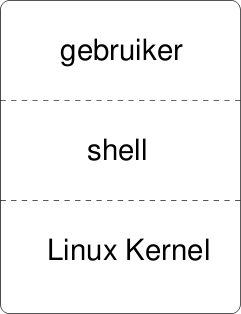
\includegraphics[scale=0.5]{images/shell_intro}
  \end{center}
  \caption{De basis}
  \label{fig:shell}
\end{figure}

De \emph{shell} staat tussen de gebruiker en het systeem in en dient als \emph{opdrachtinterpreter}. De \emph{shell} hiermee vergelijkbaar met \emph{command.com} onder \emph{DOS}. Wanneer een gebruiker een commando geeft controleerd de \emph{shell} of dit opgegeven commando correct is. Hierna zal de \emph{shell} de opdracht uitvoeren, of een foutmelding teruggeven naar de gebruiker. De \emph{shell} is hiermee de eerste laag in het besturings systeem. 

Op elk systeem is er een \emph{shell} die ervoor zorgt dat commando's worden uitgevoerd. Onder \emph{Linux} zijn er meerdere \emph{shells} zoals bijvoorbeeld de \emph{Bash-Shell}, \emph{Korn-shell} en de \emph{C-shell}.

De \emph{Bourne shell} is de \emph{shell} die origineel op de \emph{AT\&T UNIX} systemen stond onder de naam sh. \emph{Bourne Again Shell} (\texttt{bash}\index{bash}) is de opensource versie en is compitable met het orgineel. Deze \emph{shell} heeft echter wel extra mogelijkheden\footnote{Bourne Again SHell, de hoofdletters ``hell'' slaan op de problemen die sommige ermee hebben}.

Naast \emph{Bash} zijn er tegenwoordig ook nog andere afgeleiden. Een goed voorbeeld hiervan is \texttt{dash}\index{dash}, \emph{Debian Almquist Shell}. Dash komt af van de in \emph{netBSD} bekende \emph{Almquist Shell} en was naar \emph{Linux} geport in 2002 \cite{bib.dash}. Het voordeel van Dash is dat het een stuk sneller is als \emph{Bash}, maar toch nog werkt volgens de \emph{POSIX} standard.\index{POSIX} Tegenwoordig maken bijvoorbeeld \emph{Debian}\footnote{\emph{Debian} maakt vanaf de \emph{Debian Squeeze} release standaard gebruik van \emph{Dash}.} en \emph{Ubuntu} gebruik van Dash.

Een \emph{Linux} systeem is geen systeem zonder een \emph{shell}, en de scripting mogelijkheden die daardoor aanwezig zijn. Bijna alles is opgebouwd rond de \emph{shell}. Een goed voorbeeld hiervan zijn de opstart scripts in \emph{Slackware}\footnote{Dit geldt natuurlijk ook voor andere distributies}. Hieronder is een voorbeeld \emph{init} script van de \emph{OpenSSH Server}:
\begin{lstlisting}
root@slackje:/etc/rc.d# cat rc.sshd 
#!/bin/sh
# Start/stop/restart the secure shell server:

sshd_start() {
  # Create host keys if needed.
  if [ ! -r /etc/ssh/ssh_host_key ]; then
    /usr/bin/ssh-keygen -t rsa1 -f /etc/ssh/ssh_host_key -N '' 
  fi
  if [ ! -f /etc/ssh/ssh_host_dsa_key ]; then
    /usr/bin/ssh-keygen -t dsa -f /etc/ssh/ssh_host_dsa_key -N ''
  fi
  if [ ! -f /etc/ssh/ssh_host_rsa_key ]; then
    /usr/bin/ssh-keygen -t rsa -f /etc/ssh/ssh_host_rsa_key -N ''
  fi
  /usr/sbin/sshd
}

sshd_stop() {
  killall sshd
}

sshd_restart() {
  if [ -r /var/run/sshd.pid ]; then
    echo "WARNING: killing listener process only.  To kill every sshd process, you must"
    echo "         use 'rc.sshd stop'.  'rc.sshd restart' kills only the parent sshd to"
    echo "         allow an admin logged in through sshd to use 'rc.sshd restart' without"
    echo "         being cut off.  If sshd has been upgraded, new connections will now"
    echo "         use the new version, which should be a safe enough approach."
    kill `cat /var/run/sshd.pid`
  else
    echo "WARNING: There does not appear to be a parent instance of sshd running."
    echo "         If you really want to kill all running instances of sshd (including"
    echo "         any sessions currently in use), run '/etc/rc.d/rc.sshd stop' instead."
    exit 1
  fi
  sleep 1
  sshd_start
}

case "$1" in
'start')
  sshd_start
  ;;
'stop')
  sshd_stop
  ;;
'restart')
  sshd_restart
  ;;
*)
  echo "usage $0 start|stop|restart"
esac
\end{lstlisting}
Het bovenstaande script zal waarschijnlijk niet helemaal direct begrijpbaar zijn. Wel zullen de grote lijnen al zichtbaar zijn. In de volgende twee hoofdstukken zal de \emph{shell} behandeld worden, waarna het bovenstaande script duidelijk te begrijpen is. Ook zal het maken van eigen scripts hierna mogelijk zijn. 

\emph{Shell} scripting is een van de sterkste punten van \emph{Linux}, omdat het gebruikers en beheerders in staat stelt een systeem ontzettend flexibel te houden. Ook kan het laagdrempelig aan worden gepast naar eigen, specifieke wensen. 

\section{De theorie}
Voordat er uitgebreid begonnen wordt met het bespreken van de verschillende mogelijkheden in de \emph{shell} is het belangerijk om te begrijpen hoe de \emph{shell} precies werkt en wat de eisen zijn. Een uitstekende documentatie over de \emph{shell} is te vinden via \texttt{man}\index{man} \texttt{bash}\index{bash}. Hierin is een goede uitleg te vinden over de werking van de \emph{shell}. Het is mogelijk om uitgebreidere documentatie gerelateerd aan scripting op te zoeken. Een goede plek hiervoor is \emph{tldp}\cite{bib.tldp.abs}, een compleet overzicht van de functionaliteit van de \emph{Bash shell}. 

De meeste generieke beschrijving van een \emph{shell} is als volgt:
\begin{quote}
any program that users employ to type commands
\end{quote}
In \emph{UNIX} zijn er verschillende soorten \emph{Shells}. Wanneer een gebruiker inlogt in het systeem zal de \emph{shell} automatisch worden gestart. De meeste \emph{Shells} zijn hiervoor special ontwikkeld. Dit programma heet een \emph{Shell} omdat het het onderliggende operating system verbergt achter de interface van de \emph{Shell}. De \emph{Shell} beheerd de technische details van de kernel interface, welke de binnenste laag is binnen elk operating system.

Ook de grafische interfaces, zoals \emph{Gnome}, \emph{KDE} of \emph{Fluxbox} zijn \emph{Shells}. Ze worden ook wel \emph{visuele} \emph{shells} of grafische \emph{shells} genoemd. \cite{bib.shell}

\subsection{Interactive command line en scripting program language?}
Toen de \emph{UNIX shell} voor het eerst uitkwam was dit een bijzondere \emph{shell}. Er waren al wel andere \emph{Shells}, maar de \emph{Shells} welke er al wel waren waren niet en een \emph{Interactive Commandline} en een \emph{Scripting Program Language}. De \emph{UNIX shell} was dit wel, met alle voordelen van dien. Je kon nu zelf programma's draaien met de \emph{Shell} en je had dus een stuk meer vrijheid om dingen te doen. 
 
\subsection{Shebang}
Wanneer een programma gestart wordt moet de file loader van de \emph{Shell} weten waarmee het programma geopend moet worden. Standaard zal dit meestal het programma met de \emph{Shell} waarin op dat moment een gebruiker actief is. 

Het kan voorkomen dat het script met een andere \emph{shell} of binary gestart zal moeten worden. Een andere mogelijkheid is het verkrijgen van een garantie dat een bepaalde \emph{shell} het script start. Om dit doel te bereiken kan er gebruik gemaakt worden van een \emph{shebang}, een speciale eerste regel in een script. Deze \emph{shebang} ziet er als volgt uit:
\begin{lstlisting}
#!/bin/bash
\end{lstlisting}
Het hekje met het uitroepteken is de \emph{shebang}. Doordat het hekje commentaar is, zal het genegeerd worden door de interpreter. De program loader zal het echter wel lezen en de goede interpreter aanroepen. In het geval van hierboven dus de \emph{Bash shell}. Er kan op deze manier bijvoorbeeld ook eenvoudig een \emph{Perl}, \emph{PHP} of andere interpreter aangeroepen worden in de \emph{shell}. 

\subsection{Dash in Slackware?}
De standaard \emph{Shell} in \emph{Slackware} is \emph{Bash}. Het is echter mogelijk een andere \emph{shell} te kiezen. Van de \emph{Dash shell} zijn er in \emph{Slackware} geen standaard paketten, maar Ash\footnote{Dash is afgeleid van Ash} is wel beschikbaar. 

Hieronder is te zien hoe een nieuwe gebruiker wordt aangemaakt, welke gebruik zal maken van de \emph{Ash shell}:
\begin{lstlisting}
root@slackje:~# adduser dashtest
Login name for new user: dashtest
User ID ('UID') [ defaults to next available ]: 
Initial group [ users ]: 
Additional UNIX groups:
[...]
:  
Home directory [ /home/dashtest ] 
Shell [ /bin/bash ] /bin/ash
Expiry date (YYYY-MM-DD) []: 
New account will be created as follows:
---------------------------------------
Login name.......:  dashtest
UID..............:  [ Next available ]
Initial group....:  users
Additional groups:  [ None ]
Home directory...:  /home/dashtest
Shell............:  /bin/ash
Expiry date......:  [ Never ]
\end{lstlisting}
De \emph{Ash shell} uit \emph{Slackware} is niet exact hetzelfde als \emph{Bash} en \emph{Dash}. Na het inloggen zal het eerste verschil al opvallen. Ook zullen dingen als \emph{tab completion} zal niet standaard werken. Andere distributies, zoals \emph{Debian/Ubuntu} zullen standaard instellingen aanbieden waarbij dit wel mogelijk is. Om Ash zich hetzelfde te laten gedragen als \emph{Bash} zal er dus wel het een en ander moeten worden aangepast.

In de rest van dit hoofdstuk wordt er vanuit gegaan dat de standaard \emph{shell} de \emph{Bash shell} is. Het gebruik van een andere \emph{shell} is mogelijk, maar hou rekening met de verschillen tussen de \emph{shells}. 

\subsection{In en output}\index{STDOUT}\index{STDIN}\index{STDERR}
De \emph{shell} heeft, net als ieder ander proces, mogelijkheden tot in-, en output van data. De input, \emph{STDIN}, is bijvoorbeeld het toetsenbord\footnote{Dit kan ook wat anders zijn, zie de paragraaf Piping} of de muis. De output, \emph{STDOUT}, is bijvoorbeeld het scherm, of een bestand. Hiernaast is er ook nog \emph{STDERR}. Op deze \emph{stream} worden de fouten uitgevoerd. De \emph{STDERR} wordt standaard naar het scherm geschreven, maar kan ook worden doorgestuurd naar iets anders als dit nodig is. Deze \emph{streams} kunnen ook in programma's gebruikt worden. In C kunnen deze streams bijvoorbeeld gewoon met \emph{fopen()} benaderd worden. In \ref{fig:output} is een goed voorbeeld te zien van hoe de in/output werkt bij een applicatie. In principe is dit hetzelfde voor alle applicaties.
\begin{figure}[H]
  \begin{center}
    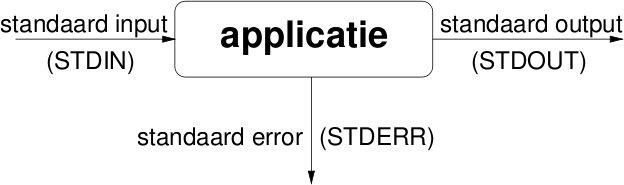
\includegraphics[scale=0.5]{images/inout}
  \end{center}
  \caption{In en Output}
  \label{fig:output}
\end{figure}
Het kunnen gebruiken van deze streams is heel belangrijk voor \emph{Shells}. Zorg dus dat de basis hiervan goed duidelijk is. 

\subsection{Pipeline}
Alle \emph{UNIX} applicaties hebben een standaard input en standaard output mogelijkheid. De \emph{shell} bied handige functionaliteit bij het doorsluizen van uitvoer met het '$|$' teken (sluis, engels: pipe). Het '$|$' teken sluist de uitkomst van de eerste opdracht naar de input van de tweede. Een kort voorbeeld:
\begin{lstlisting}q
  grep kernel /var/log/syslog | more
\end{lstlisting}
\index{cat}\index{grep}\index{more}\index{\textpipe}
\texttt{cat}\index{cat} leest een bestand uit, in dit geval de logfile /var/log/syslog. De output wordt nu gepiped naar het commando \texttt{grep}\index{grep} met een $|$. De output wordt nu niet doorgestuurd naar de \emph{stdout}, en zal dus niet worden weergeven op je scherm. Zodra \texttt{grep}\index{grep} de output ontvangt zoekt \texttt{grep}\index{grep} naar de tekenreeks die opgegeven is. Dat is in dit geval ``kernel''. Voordat het nu doorgestuurd wordt naar de \emph{stdout} wordt het eerst nog gepiped via \texttt{more}\index{more}. \texttt{more}\index{more} zorgt ervoor dat de output gestopt wordt zodra het scherm vol is. Op deze manier kan het resultaat gemakkelijk bekeken worden. Alles gelezen? Dan kan er naar de volgende buffer gegaan worden. 

\begin{lstlisting}
  grep bash /etc/passwd | sort > ~/bash_gebruikers.txt
\end{lstlisting}\index{sort}\index{grep}\index{$>$}
\texttt{grep}\index{grep} ontvangt de inhoud van de file '/etc/passwd' en doorzoekt de inhoud naar de tekenreeks ``bash''. Zit die reeks niet in een regel, dan wordt deze genegeerd. Alle regels van passwd-bestand met ``bash'' in de regels worden nu doorgesluisd naar \texttt{sort}\index{sort}. Deze plaatst ze op alfabetische volgorde. 

Net zoals bij het vorige voorbeeld ontvangt \texttt{grep}\index{grep} weer het resultaat van \texttt{cat}\index{cat}, waarbij het resultaat de inhoud van een bestand is, in dit geval /etc/passwd. Nadat er gezocht is op de string ``bash'' wordt het gepiped naar \texttt{sort}\index{sort}, welke ze sorteert op alfabetische volgorde. 

Het '$>$' teken wordt gebruikt om het resultaat op de \emph{stdout} weg te schrijven. Het resultaat wordt nu naar de file ``bash\_gebruikers'' geschreven. Let wel op dat gebruik maken van '$>$' betekend dat de file, waar de output naartoe wordt gestuurd, gewist zal worden. Om de output achter de huidige content te plakken kan er gebruik gemaakt worden van '$>>$'\index{$>>$}. Wanneer de file niet bestand zal die dan wel gemaakt worden.

Dit soort constructies stellen een gebruiker dus in staat om de uitvoer, \emph{STDOUT} via een \emph{pipeline} als invoer \emph{STDIN} naar het volgende programma te sturen. 

\subsubsection{STDERR redirecten}\index{STDERR}
Hiervoor was al te zien dat \emph{STDOUT} te redirecten is naar een bestand. Maar wat gebeurt er wanneer er fouten optreden? Die moeten misschien ook wel ergens heen. Ook de data op \emph{STDERR} is te redirecten: 
\begin{lstlisting}
cat /etc/passwd | grep test 2> grep_errors.txt
\end{lstlisting}
In het voorbeeld hierboven is te zien dat er geen gebruik gemaakt wordt van $>$ maar van 2$>$\index{2$>$}. Dit houdt in dat de fouten die eventueel optreden worden geschreven naar het bestand ``grep\_errors.txt''. De gewone output wordt nu naar \emph{STDOUT} geschreven. Deze zal niet worden opgeslagen in het bestand.

\begin{lstlisting}
cat /etc/passwd | grep test 1>&2 
\end{lstlisting}
In sommige gevallen is het handig om de output van \emph{STDOUT} te redirecten naar \emph{STDERR}. Dat is precies wat de 1$>$\&2 doet. \index{1$>$\&2}

\begin{lstlisting}
cat /etc/passwd | grep test 2>&1
\end{lstlisting}
Het is vaak veel handiger om dit precies omgekeerd te doen, ofwel de \emph{STDERR} naar \emph{STDOUT} te redirecten. En ook hier is iets voor bedacht, en wel 2$>$\&1 en dus precies het omgekeerde. Let dus goed op de syntax en kies de juiste redirect in de juiste situatie\index{2$>$\&1}.

\begin{lstlisting}
rm tmp/ -rfv &> /dev/null
\end{lstlisting}
\&$>$ zal alle output die vanaf \texttt{rm}\index{rm} afkomt van zowel \emph{STDOUT} als \emph{STDERR} worden redirect naar het opgegeven bestand. In dit geval wordt dit geredirect naar \emph{/dev/null}\index{/dev/null}.

\subsection{TAB-completion}
TAB-completion is eenvoudig en werkt erg makkelijk volgens een simpel principe:
Als er genoeg letters ingevoerd zijn zodat een bestand, opdracht, of naam van een directory kan worden achterhaalt dan vult \emph{Bash} de rest aan. Een voorbeeld:
\begin{lstlisting}
  /usr/lo [tab] wordt /usr/local
\end{lstlisting}
Als er nu op TAB wordt gedrukt vult \emph{Bash} het aan, omdat het ziet dat er gezocht wordt naar '/usr/local'.

Als er bij /usr/li op tab wordt gedrukt kan \emph{Bash} niet het juiste resultaat vinden omdat er meerdere directories zijn die beginnen met /usr/li. Als er vervolgens nogmaals op tab wordt gedrukt geeft \emph{Bash} alle mogelijkheden weer.

\subsection{Opdrachtalliassering}
\begin{lstlisting}
alias psa='ps -aux | less'
alias cp='cp -i'
alias mv='mv -i'
alias rm='rm -i'
\end{lstlisting}
Alias geeft de mogelijkheid om een commando te herschrijven met extra opties. Zet het bovenstaande voorbeeld in het bestand \emph{\~{}/.bash\_profile}\index{\~{}/.bash\_profile} in de home-directory (maak het zonodig aan). Dit bestand zijn extra configuratie instellingen voor de \emph{Bash}B \emph{shell}. Globale \emph{Bash} instellingen moeten in het bestand \emph{/etc/profile} gedaan worden. Activeer de aanpassingen door opnieuw in te loggen of via het commando \texttt{source \~{}/.bash\_profile}.\index{\~{}/.bash\_profile}

\subsection{Historylist}
\emph{Bash} onthoudt bij een sessie de uitgevoerde opdrachten. Bij het uitloggen van het systeem worden alle opdrachten in de file \emph{\~{}/.bash\_history} in de home-directory geschreven. Wanneer een gebruiker de volgende keer inlogt zal door het commando \emph{history}\index{history} precies te zien zijn wat er bij een vorige sessie is gedaan. Als er tijdens een sessie een opdracht uitgevoerd moet worden die al uitgevoerd is kan er met het pijltje-omhoog de vorige opdrachten worden geselecteerd.

Een andere functionaliteit die \emph{Bash} biedt is om een commando dat net is ingegeven te herhalen. Hiervan een korte beschouwing:
\begin{lstlisting}
  mount /dev/hdd -t iso9660 -o ro /mnt/cdrom
\end{lstlisting}
\index{mount}
Omdat dit soort lange opdrachten veel tijd kosten om in te tikken is het gemakkelijk als zo'n opdracht herhaalt moet worden. Door "!$<$commando$>$" te voer je de vorige opdracht uit. In dit geval is dat dus '!mount'.

\subsection{Jobcontrol}
Jobcontrol is mogelijk in \emph{Linux} omdat het een multi-tasking operating system is. Met job control kan in een \emph{shell} meerdere programma's tegelijkertijd worden uitgevoerd. Normaal gesproken draait een opdracht die wordt uitgevoerd op de voorgrond. Met andere worden, de prompt verschijnt pas weer als de opdracht is be\"{e}indigd. De makkelijkstse manier om een job op de achtergrond te plaatsen is door aan het einde van de opdracht een ``\&'' (ampersand) te plaatsen.\index{\&}

De volgende opdracht zoekt vanaf de root ('/') naar alle bestanden die op '.txt' eindigen en zet het resultaat ervan in het bestand 'tekstbestanden'. Doordat er een ampersand achterrstaat wordt het op de achtergrond uitgevoerd en verschijnt de \emph{shell} prompt weer. \texttt{ls -IR /}\index{ls} laat alle bestanden vanaf root zien.\index{ls}

Een op de voorgrond gestart programma kan naar de achtergrond worden gestuurd door \emph{ctrl-z}.
\index{ls}
\begin{lstlisting}
find / -name '*.txt*' > tekstbestanden &
ls -IR / &
\end{lstlisting}
Met de opdracht \index{jobs}\index{jobs} worden alle achtergrond-processen weergeven en in dit geval zou het dus de find opdracht weergeven en de ls opdracht.
\begin{lstlisting}
[1]- Running find / - name '*.txt *' > tekstbestanden &
[2]+ Running ls −lR / &
\end{lstlisting}
Wanneer 'Running' in 'Stopped' veranderd is het process gestopt. Aannemende dat het nog loopt kan het naar de voorgrond gehaald worden met \texttt{fg \%1}\index{fg} of met \texttt{fg find}. Het komt voor dat een lopende opdracht be\"{e}indigd moet worden. Met de opdracht \texttt{kill}\index{kill} is een opdracht af te breken op het \emph{PID} (process ID). Het PID is te zien door \texttt{ps -aux}\index{ps} in te geven. Ook kan \emph{KILL} lopende achtergrond processen stoppen: \index{kill}\texttt{kill \%2} zal in dit geval \texttt{ls -IR /}\index{ls} be\"{e}indigen. Mocht het voorkomen dat alle processen met een bepaalde naam be\"{e}indigd moeten worden dan zou dat het beste met \index{killall}\texttt{killall $<$naam$>$} gedaan kunnen worden.

\subsection{Patronen, Joker-tekens en Accolades}
Een krachtige optie van de \emph{Bash shell} is het gebruik van patronen om bestanden en opdrachten mee aan te duiden.

\begin{lstlisting}
  \* Staat voor 0 of meerdere willekeurige tekens (wildcard, jokerteken)
  \? Staat voor 1 willekeurig teken
  [...] Staat voor 1 van de tekens tussen de haken
  [A-F] Staat voor alle tekens tussen het eerste en tweede
  [!..] Staat voor elk ander teken dan dat er tussen de haken staat
  [!A-F] Staat dus voor elk ander dat niet tussen de A en de F zit
\end{lstlisting}
Alle bestanden van drie letters beginnende met de 'a' en eindigen op de 'z' kunnen gevonden worden met:\index{ls|(}
\begin{lstlisting}
  ls -l a?z
\end{lstlisting}
Alle bestanden die met een 'a' beginnen en eindigen op een 'z' kunnen worden weergeven met:
\begin{lstlisting}
  ls -al a*z
\end{lstlisting}
Stel er moet een lijst komen van alle bestanden beginnende met de 'a', 'b', 'c', of 'd', dan kan je dit doen met:
\begin{lstlisting}
  ls -l a* b* c* d*
\end{lstlisting}
Een iets betere oplosing is:
\begin{lstlisting}
  ls -l [abcd]*
\end{lstlisting}
Maar omdat abcd opeenvolgende letters zijn kan die het best zo worden uitgevoerd:
\begin{lstlisting}
  ls -l [a-d]*
\end{lstlisting}\index{ls|)}
Accoladen-uitbreiding is een manier om opdrachten te maken ongeacht of het bestand of de opdracht wel bestaat:
\begin{lstlisting}
  mkdir tijddir1,2,3,4
\end{lstlisting}

\subsection{Opdracht-substitutie}
Opdracht-substitutie maakt het mogelijk om de opdrachtregel door zijn resultaat te veranderen. De opdracht moet wel tussen \emph{backticks}\index{`} ` worden geplaatst. 
\begin{lstlisting}
  ls -l `find /usr/doc -name '*README*'`
\end{lstlisting}\index{ls}\index{find}
Deze opdracht zoekt naar alle '*README*' bestanden in de '/usr/doc' directory, en zorgt ervor dat \emph{find} ze \'{e}\'{e}n voor \'{e}\'{e}n aan \emph{ls -l} doorgeeft. De volgende opdracht werkt niet omdat ls de gegevens vanuit het standaard invoer kanaal negeert.
\begin{lstlisting}
  find /usr/doc/ -name `*README*` | ls -l
\end{lstlisting}
Dit is te omzijlen door \texttt{xargs}\index{xargs} toe te voegen:
\begin{lstlisting}
  find /usr/doc/ -name `*README*` | xargs ls -l
\end{lstlisting}

% tirlnx01 - Materiaal om het keuzevak Linux te geven 
% op de Hogeschool Rotterdam.
% Copyright (C) 2010 - 2011  Paul Sohier, Kevin van der Vlist
%
% This program is free software: you can redistribute it and/or modify
% it under the terms of the GNU General Public License as published by
% the Free Software Foundation, either version 3 of the License, or
% (at your option) any later version.
%
% This program is distributed in the hope that it will be useful,
% but WITHOUT ANY WARRANTY; without even the implied warranty of
% MERCHANTABILITY or FITNESS FOR A PARTICULAR PURPOSE.  See the
% GNU General Public License for more details.
%
% You should have received a copy of the GNU General Public License
% along with this program.  If not, see <http://www.gnu.org/licenses/>.
%
% Kevin van der Vlist - kevin@kevinvandervlist.nl
% Paul Sohier - paul@paulsohier.nl

\chapter{Shell scripting}
Het beheersen van \emph{UNIX} commando's en een shell script taal zijn het fundament van een goede systeembeheerder en maken zijn leven vele malen aangenamer. We gaan hieronder kort de basis uitleggen van shell scripting. Dit is de pure basis, hierna zal het \emph{SSH} script van het vorige hoofdstuk kunnen begrijpen en waarschijnlijk ook na kunnen maken. De rest van dit hoofdstuk zal gaan over Statements, functies, en structuren. Maar ook over het gebruik van andere programmeer talen, en commando's.

\section{Statements, expressies en controle structuren}
Een belangerijk onderdeel van elke programmeer taal zijn de aanwezige statements. Het lijk eigenlijk erg op elkaar lijkt als je een normale programmeer taal zalt vergelijk met \emph{Bash}, maar het is toch weer niet helemaal hetzelfde. We gaan er een beetje van uit dat je de basis van programmeren wel kent, en ongeveer weet wat wat het doet. 

\section{Variabelen en het if-statement}
Variabelen bieden de mogelijkheid om tijdelijk dingen op te slaan. De \emph{Bash-shell} maakt weinig onderscheid in type variabelen zo bestaaan er wel integers en strings, maar zijn er bijvoorbeeld geen doubles of andere \emph{datatypen}.

Zet het onderstaand voorbeeld in het bestand 'script.sh'. Maak het executable door \texttt{chmod + x}, en roep het daarna aan met \texttt{./script.sh}.\index{chmod}

\begin{lstlisting}
#!/bin/bash
echo "Hey, wat is je naam?"
read naam
if [ $naam == $LOGNAME ]; then
    echo "Ha $naam"
else
    echo "Dat is niet waar!"
fi
exit
\end{lstlisting}%$
Op de eerste regel staat \emph{\#!/bin/bash}, dit geeft aan dat dit een shellscript is. Ondanks dat het geen vereiste is om een werkend script te maken wordt het vaak wel gebruikt. Soms wordt bash vervangen door sh.

Het commando \texttt{echo}\index{echo} zet iets op het scherm waarna \texttt{read}\index{read} de input van de gebruiker opslaat in de variable 'naam'. Het if-statement vergelijkt de waarde van de variable naam met de waarde in de \emph{variable \$LOGNAME}\index{\$LOGNAME}. Wanneer ze overeen komen (==) dan voert de shell de regel onder het if-statement uit, en anders voert de shell het \emph{else-statement} uit. De variable LOGNAME is een systeem-variable die de inlognaam van de user bevat. Als er met de waarde in een variable wordt gewerkt moet er een \$ voor komen.

De structuur van het \emph{if-statement}:
\begin{lstlisting}
if conditie 1
    then
    statement1
    statement2
    ........
elsif conditie2
    then
    statement3
    statement4
    ........
elsif conditie3
    then
    statement5
    statement6
    ........
fi
\end{lstlisting}

\section{Systeem variabelen}
Hierboven maakten we al gebruik van \emph{systeem} variabelen, welke door de \emph{Shell} zelf een waarde gegeven wordt. Naast \emph{\$LOGNAME} zijn dit een aantal belangrijke voorbeelden:
\begin{itemize}
\item \emph{\$UID}: Bevat welke \emph{real} user ID de ingelogde gebruiker is.
\item \emph{\$DISPLAY}: Bevat welk display er op dat moment op gewerkt wordt.
\item \emph{\$PATH}: In dit pad worden de programma's/commando's gezocht welke uitgevoerd worden. Dit moet bijvoorbeeld aangepast worden wanneer je een programma op een ander als standaard locatie installeert.
\end{itemize}
We kunnen uiteraard niet alle aanwezige \emph{systeem} variabelen hier gaan noemen. Als je op internet of in de \emph{man pages} zoekt kan er nog veel meer voorbeelden vinden als hierboven.

\section{Expressies}
\emph{Expressies} worden vaak gebruikt bij het testen van \emph{voorwaarden}. Er wordt gekeken of er aan een bepaalde voorwaarde wordt voldaan. Aan de hand van de uitkomst van de voorwaarde wordt er een stuk code uitgevoerd.

\subsection{String expressies}
\begin{tabular}[t]{ll}
  Expressie & Waar als\ldots \\
  \hline
  -z string & de lengte van de string 0 is \\
  -n string & de lengte van string niet 0 is\\
  string1 == string2 & de twee strings gelijk zijn\\
  string1 != string2 & de twee strings ongelijk zijn\\
  string & de string niet NULL is\\
\end{tabular}

\subsection{Integer expressies}
\begin{tabular}[t]{ll}
  expressie & waar als\ldots \\
  \hline
  int1 -eq int2 & de eerste integer gelijk is aan de tweede integer (equal)\\
  int1 -ne int2 & de eerste integer ongelijk is aan de tweede integer (not equal)\\
  int1 -gt int2 & de eerste integer groter is als de tweede integer (greater) \\
  int1 -ge int2 & de eerste integer groter of gelijk is aan de tweede integer (greater or equal) \\
  int1 -lt int2 & de eerste integer lager is als de tweede integer \\
  int1 -le int2 & de eerste integer lager of gelijk is aan de tweede integer \\
\end{tabular}

\subsection{Bestands expressies}\label{h7.bestandexp}
\begin{tabular}[t]{ll}
  Expressie & Waar als\ldots\\
  \hline
  -e file & file bestaat \\
  -r file & file bestaat en is readable \\
  -w file & file bestaat en is writeable \\
  -x file & file bestaat en is executable \\
  -f file & file bestaat en is een gewoon bestand \\
  -d file & file bestaat en is een directory \\
  -h file & file bestaat en is een symbolic link \\
  -c file & file bestaat en is een character special file \\
  -b file & file bestaat en is een block special file \\
  -p file & file bestaat en is een named pipe \\
  -u file & file bestaat en is setuid \\
  -g file & file bestaat en is setgid \\
  -k file & file bestaat en heeft een sticky bit \\
  -s file & file bestaat en de grote is meer als 0 \\
\end{tabular}

Een voorbeeld van een expressie is als volgt:
\begin{lstlisting}
  if [ -e /tmp/test/ ]; then
      echo ``/tmp/test/ bestaat!''
  fi
\end{lstlisting}

\subsection{Logische operatoren}
\begin{tabular}[t]{ll}
  Expressie & Doel
  \\
  \hline
  ! & neem het tegenovergestelde van het resultaat van de expressie \\
  -a & AND operator \\ 
  -o & OR operator \\
 \end{tabular}

\section{De shell parameter variabelen}\label{h7.para}
\begin{tabular}[t]{ll}
  Variabele & Doel \\
  \hline
  \$0 & Naam van het script\\
  \$1 tot \$9 & Het eerste tot de negende parameter\\
  \$\# & Het totaal aantal parameters \\
  \$* & Alle parameters die zijn opgegeven \\
  \$@ & Alle parameters als gescheiden woorden \\
\end{tabular}

\section{Het case-statement}
Het \emph{case-statement}, maakt gebruik van het voorkomen van bepaalde \emph{cases} die in het script voorkomen. Er is van te voren al gedacht over de mogelijk uitvoer en springt daar op in. Maak de file 'case.sh' aan met de onderstaande code erin. Maak de file executable en voer het uit.
%todo: Code controleren (Echo!)
\begin{lstlisting}
#!/bin/bash
echo -n "$*"
case $2 in
    "-")
        echo 'expr $1 - $3'
        ;;
    "+")
        echo 'expr $1 + $3'
        ;;
    "*")
        echo 'expr $1 * $3'
        ;;
esac
exit
\end{lstlisting}

Op de tweede regel staat de opdracht \texttt{echo}\index{echo} die de waarde van alle variables die als parameter zijn opgegeven aan het script weergeeft (\$*). Dus als we vanuit de shell intikken './case 2 + 3' dan is de \$* gelijk aan '2 + 3'. De optie 'echo -n' zorgt ervoor dat er nog niet op een nieuwe regel wordt begonnen.

De shell leest nu het case-statement. Het vergelijkt de tweede parameter (\$2) met een '-' of '+'. Mochten ze niet overeen komen dan voert hij de code uit die bij de wildcard (*) staat. De wildcard staat voor alle mogelijk tekens. De werking van het scripot is dus een comandline rekenmachine die getallen optelt en aftrekt.

De structuur van het case statement:
\begin{lstlisting}
  case "variable" in
      mogelijkheid1)
          statement1
          statement2
          ........
      mogelijkheid2)
          statement3
          statement4
          ........
  esac
\end{lstlisting}

\subsection{Case voorbeeld}
Het volgende voorbeeld drukt telkens de komende dag af. Sla het op in de file morgen.sh, maak het executable en run het:
\begin{lstlisting}
#!/bin/bash
date=date
	case "`$date +%a`" in
	Sun) echo Sunday ;;
	Mon) echo Tuesday ;;
	Tue) echo Wednesday ;;
	Wed) echo Thursday ;;
	Thu) echo Friday ;;
	Fri) echo Saterday ;;
	Sat) echo Sunday ;;
	*) echo "Help! Onmogelijk om hier te komen!" ;;
esac
\end{lstlisting}%$
Het script maakt op dezelfde manier als het voorbeeld hiervoor gebruik van het case-statement. Alleen neemt het nu als voorwaarde het eerste woord van \texttt{date} als resultataat. Het commando \texttt{date}\index{date} wordt aan de variabele \$date toegekent. Normaal doet het commando date dit: 
\begin{lstlisting}
paul@slackbak:~$ date
Mon Dec 20 13:55:43 CET 2010
\end{lstlisting}%$
Maar '\$date +\%a' is nu dus Mon, omdat \$date het hele resultaat weergeeft. Als er '\$date + \%b' had gestaan was het resultaat Dec. Dit klinkt nogal abstract maar met een paar oefeningen is het goed te begrijpen.

\subsection{HELP, dit script werkt niet!}
Heb je het script netjes overgenomen, maar je krijgt "Help! Onmogelijk om hier te komen!"? Dat kan best. Het huidige script gaat ervan uit dat je Engels als standaard taal gebruikt. Dit is standaard bij in ieder geval \emph{Slackware}, maar mogelijk bij een andere distributie niet. Op mijn laptop, met Nederlandse instellingen, krijg ik netjes deze fout. Hoezo? Date geeft iets anders terug:
\begin{lstlisting}
paul@paul-laptop:/tmp$ date
wo dec  8 18:39:39 CET 2010
\end{lstlisting}%$
Wat valt op? Juist, er staat geen Wed, maar wo. Het case statement zal dus nooit uitgevoerd worden! Hoe kan je dit oplossen? In dit geval vrij simpel, door expliciet de taal op te geven. Voor engels kan je dit doen door als taal C te gebruiken. Dit kan op de volgende manier:
\begin{lstlisting}
paul@paul-laptop:/tmp$ LANG=C ./morgen.sh 
Thursday
\end{lstlisting}%$
Bij het maken van een \emph{Shell} script moet je altijd rekening houden met de taal van de gebruiker en het operating system. Er kan nooit van uitgegaan worden dan een gebruiker de standaard instelling of taal gebruikt. Eigenlijk kan er dus nooit in een \emph{shell} script gecontroleerd worden op taal specifieke uitingen.

\section{Het while statement}
Het \emph{while-statement} voert een bepaalde handeling uit totdat er aan een voorwaarde wordt voldaan. Hier een voorbeeldje, het script simuleert een dobbelsteen waarvan je het aantal ogen moet raden:
\begin{lstlisting}
  #!/bin/bash
  trap 'echo bedankt voor het spelen. ' EXIT
  magischnr=$(($RANDOM%6+1))
  
  while [ "$gok" != "$magischnr" ]; do
      echo Geef een cijfer tussen de 1 en de 6;
      read gok
  done
  echo "Het magische nummer was: $magischnr"
  exit
\end{lstlisting}%$
Het \texttt{trap}\index{trap} commando vangt de afbraak van het script af. Als er tijdens het runnen van het script plots op ctrl+c wordt gedrukt voert de shell het commando na de \texttt{trap} uit. Maar ook als het script netjes wordt afgesloten wordt hetr commando uitgevoerd. Meestal bevat een \texttt{trap} het verwijderen van tijdelijke files en weergeven van een afsluitboodschap. 

De structuur van het while statement:
\begin{lstlisting}
  while conditie
    do
       statement1
       statement2
       ........
 done
\end{lstlisting}

\section{Het untill-Statement}
Het \emph{until-statement} voert iets uit tot dat aan de voorwaarde wordt voldaan. Het lijkt op het while statement, alleen doet het een handeling pas als er aan een voorwaarde wordt voldaan, terwijl het while-statement zo lang er aan de voorwaarde wordt voldaan iets doet.

De structuur van het until statement:
\begin{lstlisting}
  until conditie
    do
       statement1
       statement2
       ........
 done
\end{lstlisting}
Voorbeeld:
\begin{lstlisting}
  until ["$1" = ""]
    do
       statement1
       statement2
       ........
 done
\end{lstlisting}%$

\section{Het for-statement}
Naast de while en Untill loop hebben we ook nog de for loop. De for loop wijkt iets af van de uit \emph{C} of \emph{JAVA} bekende for loop. Er is standaard een teller, en die loopt een string af. 

\begin{lstlisting}
        #!/bin/bash
        for i in `seq 1 10`;
        do
                echo $i
        done    
\end{lstlisting}%$
\emph{seq}\index{seq}\index{echo} print een sequence of nummers, in dit geval van 1 tot 10. De for loop zal hierna van 1 tot 10 tellen. De i is een variable welke gebruikt wordt als teller.

De structuur van de for loop is als volgt:
\begin{lstlisting}
for i in "$string";
do
    statement1
    statement2
    ........
done
\end{lstlisting}%$

\section{Functies}
In bijna elke taal zijn er functies aanwezig. Functies zijn handig binnen gebruik van programmeertalen, om bijvoorbeeld de code overzichtelijk te houden, veel voorkomende taken uit te voeren, of voor recursie.
Ook in de \emph{shell} zijn functies aanwezig. In het geval van een functie roep je hem gewoon aan, net als een programma.
Maak een bestand genaamd aanwezig.sh en zet het volgende script erin, en voer het hierna uit:
\begin{lstlisting}
#!/bin/bash
aanwezig() {
  if [ -e test.txt ] ; then
      echo "bestaat"
  else
      echo "bestaat niet"
  fi
}
aanwezig 
\end{lstlisting}Dit script maakt eerst een functie genaamd aanwezig. In deze functie is een controle of het bestand test.txt bestaat. (Zie paragraaf \ref{h7.bestandexp} voor uitleg over -e). Wanneer hij niet bestaat print hij dit netjes, en zodra hij bestaat print hij dit ook. Als laatste is nog de functie aanroep zelf. Dit is netals een bestand aanroepen, gewoon de functie naam.
Een voorbeeld uitvoer is dit:
\begin{lstlisting}
paul@slackje:~$ ./aanwezig.sh 
bestaat niet
paul@slackje:~$ touch test.txt
paul@slackje:~$ ./aanwezig.sh 
bestaat
paul@slackje:~$ 
\end{lstlisting}
In het eerste geval bestaat het bestand test.txt niet. Hierna wordt het bestand aangemaakt met het commando touch\index{touch}. Wanneer dit aangemaakt is, wordt het script nogmaals uitgevoerd. En nu bestaat hij!

\subsection{Parameters}
Het bovenstaande script is nog niet erg dynamische. Het zal altijd controleren voor \'{e}\'{e} bepaald bestand. Wat je dus eigenlijk wilt is dat je dynamische kan opgeven om welk bestand dit gaat. Gelukkig is dit mogelijk, en wel op de volgende manier. Sla het volgende voorbeeld op als aanwezig2.sh:
\begin{lstlisting}
#!/bin/bash
aanwezig() {
  if [ -e $1 ] ; then
      echo "$1 bestaat"
  else
      echo "$1 bestaat niet"
  fi
}
aanwezig test.txt
aanwezig aanwezig2.sh
\end{lstlisting}%$
Dit script zal als voorbeeld dit als resultaat geven:
\begin{lstlisting}
paul@slackje:~$ ./aanwezig2.sh 
test.txt bestaat niet
aanwezig2.sh bestaat
paul@slackje:~$ touch test.txt
paul@slackje:~$ ./aanwezig2.sh 
test.txt bestaat
aanwezig2.sh bestaat
\end{lstlisting}%$
Het bovenstaande script is eigenlijk maar heel weinig veranderd. In plaats van test.txt staat er nu \$1. De \$1 staat voor de eerste parameter aan die \textbf{functie} (Heeft het script ook als script parameters, dan zijn die niet zichtbaar voor de functie. Wil je de bestandsnaam toch zichtbaar maken, zal die apart op moeten geven worden als parameter). Dezelfde opties als voor de shell parameters uit paragraaf \ref{h7.para} gelden hier ook. Naast dat we afdrukken of het bestand dan daardwerkelijk bestaat, drukken we nu ook de bestandsnaam mee af. Dit zodat we kunnen zien wat de parameter eigenlijk was.
De functie aanroep wordt nu ook aangepast. Als parameter moet er nu de bestandsnaam voor de controle worden opgegeven. Normaal gesproken zouden we ook nog moeten controleren of de parameter niet leeg is. Dit hebben we echter in dit voorbeeld weggelaten.

\subsection{Shell parameters en functie parameters}
Om het eerdere script nu nog iets verder aan te passen kunnen we ook nog de parameter dynamische maken door hem op te laten geven als shell parameter. Sla onderstaande code op als aanwezig3.sh.
\begin{lstlisting}
#!/bin/bash
aanwezig() {
  if [ -e $1 ] ; then
      echo "$1 bestaat"
  else
      echo "$1 bestaat niet"
  fi
}
aanwezig $1
\end{lstlisting} 
Wat je hier ziet is dat de eerste Shell parameter direct doorgegeven wordt als parameter voor de functie, en daar wordt gebruikt. \$0 is de bestandsnaam van het Shell script, \$1 de eerste parameter. Zie ook paragraaf \ref{h7.para}.
Voorbeeld uitvoer:
\begin{lstlisting}
paul@slackje:~$ ./aanwezig3.sh 
 bestaat
paul@slackje:~$ ./aanwezig3.sh test.txt
test.txt bestaat niet
paul@slackje:~$ touch test.txt
paul@slackje:~$ ./aanwezig3.sh test.txt
test.txt bestaat
\end{lstlisting}
Zoals je ziet mist de controle op een lege parameter, en geeft hij dus dat een lege file aan als bestaat. Hierna wordt netjes gecontroleerd of test.txt aanwezig is.

\section{Arrays}
Met shell scripting kan er ook gebruik gemaakt worden van \index{array}arrays. Alhoewel deze datasets hetzelfde zijn als in de meeste andere talen, is het syntactisch wel een vreemde eend. Er zullen daarom wat voorbeelden gegeven over het gebruik van arrays:

\subsection{Assignment}
Array assignment. De quotes dienen om aardbei ijs als een element te specificeren.
\begin{lstlisting}
arr=( appel peer banaan "aardbei ijs" )
# Dit geeft dus de volgende array:
arr[0] = appel
arr[1] = peer
arr[2] = banaan
arr[3] = aardbei ijs
\end{lstlisting}

Ook kan de array assignment op specifieke locaties plaatsvinden:
\begin{lstlisting}
arr=( [0]=appel [11]="aardbei ijs" )
\end{lstlisting}

\subsection{Benaderen}
Print het tweede element:
\begin{lstlisting}
echo ${arr[1]}} 
\end{lstlisting}%$

Print de complete array:
\begin{lstlisting}
echo ${arr[@]}
\end{lstlisting}%$

Print de array size:
\begin{lstlisting}
echo ${#arr[@]}
\end{lstlisting}%$

Voeg een element toe aan de eerste vrije locatie
\begin{lstlisting}
arr[${#arr[@]}]="nieuw"
\end{lstlisting}%$

Print de size van het tweede array element 
\begin{lstlisting}
echo ${#arr[1]}
\end{lstlisting}%$

Print 2 elementen na id 10 
\begin{lstlisting}
echo ${arr[@]:10:2}
\end{lstlisting}%$

Er is nog veel meer mogelijk met arrays, maar de meest gebruikte vormen zijn nu gegeven. Mocht er meer interesse zijn in de mogelijkheden kan er naar de \emph{Advanced Bash Scripting Guide}\cite{bib.tldp.abs} gekeken worden. 

\section{En nu?}
Nu je de basis van shell scripting hebt gehad, kan je als het goed is het van SSH uit het vorige hoofdstuk compleet uit leggen hoe het werkt. Probeer zelf te bedenken hoe dit script werkt en wanneer je het niet snapt, lees de theorie nogmaals eens door en vraag je af wat je niet snapt. 

\section{Commando gebruik}
Met alleen structuren kom je natuurlijk nergens. In veel programeer talen zijn standaard functies aanwezig welke bepaalde taken kunnen doen. Met Shell scripting zal je hiervoor vaak moeten terugvallen op de standaard aanwezige commando's. Netals in de Shell zelf kan je in een Shell script standaard gebruik maken van de aanwezige commando's in de Shell. Voordat je deze gaat gebruiken moet je wel goed nadenken over wat voor consequenties dit heeft en hoe je dit kan opvangen. 

We kunnen hier niet even alle commando's welke aanwezig zijn standaard in linux gaan uitleggen. Op een standaard Slackware install zijn dit er ruim 2600, en dit document is al lang genoeg. De belangrijkste commando's kan je lezen in hoofdstuk \ref{h.basis}. Elk commando aanwezig in je distributie kan je in principe gebruiken in je Shell script. Hou er wel rekening mee dat je bijvoorbeld in een \emph{cron} niet vraagt om user input. 

\section{Alternatieve scripting mogelijkheden}
Scripting is iets wat niet alleen mogelijk is door gebruik te maken van een van de \emph{shells} op het systeem, maar dit kan ook gedaan worden met behulp van andere scripting talen. 

Een veel gebruikte scripting-, en programmeer taal is \texttt{perl}\index{perl}\cite{bib.perl.wiki}\cite{bib.perl.doc}. De afkorting \emph{perl} staat voor \emph{Practical Extraction and Report Language}, een naam die zeker recht wordt aangedaan. 

\texttt{perl}\index{perl} is een scripting taal die erg gemakkelijk gebruikt kan worden om files (of streams) te analyseren. Dit komt omdat \texttt{perl}\index{perl} een enorme ondersteuning voor \emph{reguliere expressies} heeft. 

Eem een klein idee te geven over de syntax van een \texttt{perl}\index{perl} programma zal hieronder een klein scriptje te vinden zijn wat gebruikers uit het bestand \emph{/etc/passwd} haald wanneer het \emph{uid} van de betreffende gebruiker tussen de 0 en de 999 ligt. Ook zal de gebruiker zijn wachtwoord in \emph{/etc/shadow} moeten hebben staan, of zal de login geblokkeerd moeten zijn. Het zal, wanneer de user gebruik maakt van de \texttt{sh}\index{sh} shell, deze omzetten naar \texttt{false}\index{false}. Dit zal dan worden geprint:
\begin{lstlisting}
#!/usr/bin/perl
open F, "/etc/passwd" or exit;
foreach my $line (<F>) {
    if($line =~ m/[a-z]+:[x|!]:\d{1,3}:/) {
        $line =~ s/\/sh/\/false/;
        print $line;
    }
}
\end{lstlisting}
Zoals te zien biedt het gebruik van \texttt{perl}\index{perl} een andere kijk op het toepassen van \emph{scripting}. Het is ook zo dat er niet alleen gebruik gemaakt kan worden van \texttt{perl}\index{perl}, ook \texttt{python}\index{python} is een taaltje wat vaak voor dit soort doeleinden wordt gebruikt. 

% Appendix:
\appendix
% tirlnx01 - Materiaal om het keuzevak Linux te geven 
% op de Hogeschool Rotterdam.
% Copyright (C) 2010 - 2011  Paul Sohier, Kevin van der Vlist
%
% This program is free software: you can redistribute it and/or modify
% it under the terms of the GNU General Public License as published by
% the Free Software Foundation, either version 3 of the License, or
% (at your option) any later version.
%
% This program is distributed in the hope that it will be useful,
% but WITHOUT ANY WARRANTY; without even the implied warranty of
% MERCHANTABILITY or FITNESS FOR A PARTICULAR PURPOSE.  See the
% GNU General Public License for more details.
%
% You should have received a copy of the GNU General Public License
% along with this program.  If not, see <http://www.gnu.org/licenses/>.
%
% Kevin van der Vlist - kevin@kevinvandervlist.nl
% Paul Sohier - paul@paulsohier.nl

\chapter{Slackware installeren op VirtualBox}\label{app.virtualbox}
Wanneer er geen computer vrij is om een nieuwe installatie op uit te voeren, is er de mogelijkheid om gebruik te maken van virtualisatie software. Een erg goed werkende, maar eenvoudige oplossing hiervoor is het gebruik van \emph{VirtualBox}\cite{bib.vbox}. Je kan hier eenvoudig een virtuele computer cre\"{e}eren waar je vervolgens de installatie op uit kunt voeren.

\emph{Virtualbox} kan eenvoudig geinstalleerd worden. Op \emph{Windows}, \emph{Solaris} of \emph{OS X} download je de installer van de virtualbox site. Onder \emph{Linux} staat virtualbox meestal in de gebruikte package manager van de gebruikte distributie.

De installatie van \emph{Slackware} is eigenlijk hetzelfde als normaal. Je mount de ISO van \emph{Slackware} in de instellingen van \emph{Virtualbox}. Hierna kan de VM gestart worden. Nu komt er een scherm krijgen met hierin de monitor over de VM. Volg hier gewoon alle normale installatie stappen uit hoofdstuk \ref{h.inst}.

Zodra je klaar bent met de installatie moet je zelf de installatie CD unmounten via de instellingen. Wanneer je dit niet doet zal je iedere keer opnieuw booten in de installatie CD.

\section{Problemen met netwerk/SSH}
\emph{Virtualbox} maakt standaard gebruik van NAT. Je kan dus niet zomaar bij een virtuele machine komen. Het kan echter wenselijk zijn om bepaalde services van de VM te ontsluiten, zodat je bijvoorbeeld naar de virtuele machine kan SSH'en. Dit is heel simpel te bereiken door op de \emph{host} het volgende uit te voeren:
\begin{lstlisting}
kevin@iusaaset:~$ VBoxManage modifyvm "Slackware-current-i686" --natpf1 "guestssh,tcp,127.0.0.1,2022,,22"
\end{lstlisting}%$
\emph{Slackware-current-i686} is natuurlijk de naam van de VM. Verder staat hier dat je onder het label \emph{guestssh}, met het TCP protocol verkeer gericht op 127.0.0.1:2022 wil forwarden naar guest:22. 

Voer dit uit als de VM uit staat, en na het aanzetten van de VM is hij beschikbaar.

% tirlnx01 - Materiaal om het keuzevak Linux te geven 
% op de Hogeschool Rotterdam.
% Copyright (C) 2010 - 2011  Paul Sohier, Kevin van der Vlist
%
% This program is free software: you can redistribute it and/or modify
% it under the terms of the GNU General Public License as published by
% the Free Software Foundation, either version 3 of the License, or
% (at your option) any later version.
%
% This program is distributed in the hope that it will be useful,
% but WITHOUT ANY WARRANTY; without even the implied warranty of
% MERCHANTABILITY or FITNESS FOR A PARTICULAR PURPOSE.  See the
% GNU General Public License for more details.
%
% You should have received a copy of the GNU General Public License
% along with this program.  If not, see <http://www.gnu.org/licenses/>.
%
% Kevin van der Vlist - kevin@kevinvandervlist.nl
% Paul Sohier - paul@paulsohier.nl

\chapter{BIOS}
De BIOS is een belangrijk onderdeel van je computer. BIOS staat voor \emph{Basic Input Output System}. Zonder BIOS zal je PC nooit werken. Wanneer je je PC opstart is het eerste wat je ziet je BIOS, nog voordat het operating system gestart is. De BIOS zal je basis hardware controleren en regelt alle communcatie tussen het operating system en de hardware. 

In elke BIOS zijn instellingen aan te passen, en vaak heb je deze nodig om bijvoorbeeld Linux te kunnen installeren. 

\section{Boot sequence}
Om Linux te kunnen installeren moet er vaak vanaf een ander medium als de aanwezige harde schijf opgestart worden. In veel gevallen is dit echter standaard uitgeschakeld en moet je de BIOS instellingen aanpassen naar je eigen wens zodat je van bijvoorbeeld CD of USB stick kan booten.
Om dit te doen moet je opstarten in de BIOS. Vaak doe je dit door een toets zoals F2 of del in te drukken, welke dit is hangt af van de gebruikte hardware en wordt vaak weergeven bij het opstarten.

Zodra je in de BIOS bent zal je op zoek moeten gaan naar de plek waar je de boot sequence aan kan passen. Vaak is dit een apart tabblad dat Boot Sequence heet. In dit tabblad zal je de sequence zo moeten aanpassen dat jou installatie medium voor de harde schijf staat. Zodra je dit gedaan hebt kan je het opslaan en opnieuw opstarten. Als het goed is start je PC nu op vanaf jou installatie medium.

% tirlnx01 - Materiaal om het keuzevak Linux te geven 
% op de Hogeschool Rotterdam.
% Copyright (C) 2010 - 2011  Paul Sohier, Kevin van der Vlist
%
% This program is free software: you can redistribute it and/or modify
% it under the terms of the GNU General Public License as published by
% the Free Software Foundation, either version 3 of the License, or
% (at your option) any later version.
%
% This program is distributed in the hope that it will be useful,
% but WITHOUT ANY WARRANTY; without even the implied warranty of
% MERCHANTABILITY or FITNESS FOR A PARTICULAR PURPOSE.  See the
% GNU General Public License for more details.
%
% You should have received a copy of the GNU General Public License
% along with this program.  If not, see <http://www.gnu.org/licenses/>.
%
% Kevin van der Vlist - kevin@kevinvandervlist.nl
% Paul Sohier - paul@paulsohier.nl

\chapter{Partities en fdisk}\label{app.fdisk}
Een harddisk wordt meestal ingedeeld in partities. Voor de installtie van \emph{Linux} moeten er minimaal twee partities worden gemaakt. \'{E}\'{e}n partitie voor het algemene \emph{Linux filesysteem} en \'{e}\'{e}n partitie voor swap. Windows partitioneerd verplicht in een primaire en een extended partitie. Binnen de extended partitie kunnen vervolgens werer enkele logical partities aangemaakt worden. \emph{Linux} ondersteund echter meerdere primaire partities.

\section{Fdisk}
Om je SATA schijf te partioneren moet je het volgende commando gebruiken:
\begin{lstlisting}
fdisk /dev/sda
\end{lstlisting}
Dit commando zal de eerste aanwezige schijf nemen. Wil je een andere schijf? Verander dan de sda in bijvoorbeeld sdb. Als je het niet zeker weet, kan je via het command
\begin{lstlisting}
dmesg | less
\end{lstlisting}dit vinden. \index{dmesg}\index{less}

Type nu eerst m in om te zien welke opties fdisk allemaal heeft. Je krijgt onderstaand scherm:
\begin{lstlisting}
root@slackje:~# fdisk /dev/sda

Command (m for help): m
Command action
   a   toggle a bootable flag
   b   edit bsd disklabel
   c   toggle the dos compatibility flag
   d   delete a partition
   l   list known partition types
   m   print this menu
   n   add a new partition
   o   create a new empty DOS partition table
   p   print the partition table
   q   quit without saving changes
   s   create a new empty Sun disklabel
   t   change a partition's system id
   u   change display/entry units
   v   verify the partition table
   w   write table to disk and exit
   x   extra functionality (experts only)

Command (m for help): 
\end{lstlisting}
Kies vervolgens 'p' om de huidige partitie instellingen te tonen.

\begin{lstlisting}
Command (m for help): p

Disk /dev/sda: 26.8 GB, 26843545600 bytes
255 heads, 63 sectors/track, 3263 cylinders, total 52428800 sectors
Units = sectors of 1 * 512 = 512 bytes
Sector size (logical/physical): 512 bytes / 512 bytes
I/O size (minimum/optimal): 512 bytes / 512 bytes
Disk identifier: 0x028f6a13

   Device Boot      Start         End      Blocks   Id  System
/dev/sda1   *          63    10506509     5253223+  83  Linux
/dev/sda2        10506510    41977844    15735667+  83  Linux
/dev/sda3        41977845    52420094     5221125   82  Linux swap
\end{lstlisting}
Hier zijn al drie partities aanwezig. Deze handleiding gaat er van uit dat er geen partities aanwezig zijn, en deze partities hierboven zullen dan ook niet meer genoemd worden hieronder. Wanneer dit wel het geval is moet het eerstvolgende volg nummer gekozen worden. In dit geval is dat 4. Deze waarde moet onthouden worden. Kies vervolgens 'n' om een partitie toe te voegen.
\begin{lstlisting}
Command (m for help): n
Command action
   e   extended
   p   primary partition (1-4)
p
Partition number (1-4, default 1): 1
First sector (2048-52428799, default 2048): 2048
Last sector, +sectors or +size{K,M,G} (2048-52428799, default 52428799): +10240M
\end{lstlisting}
Na 'n' is achtereenvolgens gekozen voor 'p', '1', '1'\footnote{In het voorbeeld is gekozen voor 2048, omdat deze harde schijf in gebruik is. Echter, bij een nieuwe installatie kies je voor 0.}  en '+10240M'. De 'p' staat voor primary partitie en de '1' voor het nummer. Vervolgens wordt om het cylinder nummer gevraagd. De waarde '1' geeft aan dat het begin van de harddisk gekozen wordt. Vervolgens dient de eind-cylinder van de partitie gegegeven te worden. De waarde '+10240M' staat voor 10 gigabte.
Nu de hoofdpartitie is aangemaakt kan de swap partitie gemaakt worden. Hiervoor kan dezelfde procedure gebruikt worden, namelijk: 'n', 'p', '2', 'enter', '+128M' (Of meer\footnote{Het best kan je kiezen voor een SWAP partitie van 2 maal je RAM geheugen. Als je dus 2GB RAM hebt kan je het beste 4GB swap nemen.}). Nu is de tweede partitie aangemaakt met een grote die jij zelf gekozen hebt. Kies vervolgens 'p' om de partitie tabel te weergeven.
\begin{lstlisting}
Command (m for help): n
Command action
   e   extended
   p   primary partition (1-4)
p
Partition number (1-4, default 2): 
Using default value 2
First sector (20973568-52428799, default 20973568): 
Using default value 20973568
Last sector, +sectors or +size{K,M,G} (20973568-52428799, default 52428799): +128M

Command (m for help): p

Disk /dev/sda: 26.8 GB, 26843545600 bytes
255 heads, 63 sectors/track, 3263 cylinders, total 52428800 sectors
Units = sectors of 1 * 512 = 512 bytes
Sector size (logical/physical): 512 bytes / 512 bytes
I/O size (minimum/optimal): 512 bytes / 512 bytes
Disk identifier: 0x028f6a13

   Device Boot      Start         End      Blocks   Id  System
/dev/sda1            2048    20973567    10485760   83  Linux
/dev/sda2        20973568    21235711      131072   83  Linux
\end{lstlisting}
De paritite tabel geeft 2 partities weer. Beide hebben id 83 (Linux native). Dit is het standaard Linux type. Voor de tweede partitie moet dit veranderd worden in id 82 (Linux swap).
Kies 't' voor het veranderen van het type, en vervolgs het partitie nummer '2'. Nu kan het id gegeven worden (82), of via de letter 'L' kan er een lijst van typen worden opgevraagd. Na het veranderen van het type kan via de optie 'p' een nieuw partitie overzicht gevraagd worden. Dit zal er dan zo uit zien:
\begin{lstlisting}
Command (m for help): t
Partition number (1-4): 2
Hex code (type L to list codes): 82
Changed system type of partition 2 to 82 (Linux swap)

Command (m for help): p

Disk /dev/sda: 26.8 GB, 26843545600 bytes
255 heads, 63 sectors/track, 3263 cylinders, total 52428800 sectors
Units = sectors of 1 * 512 = 512 bytes
Sector size (logical/physical): 512 bytes / 512 bytes
I/O size (minimum/optimal): 512 bytes / 512 bytes
Disk identifier: 0x028f6a13

   Device Boot      Start         End      Blocks   Id  System
/dev/sda1            2048    20973567    10485760   83  Linux
/dev/sda2        20973568    21235711      131072   82  Linux swap
\end{lstlisting}
Als laatste moet de optie 'a' gekozen worden om partitie '1' bootable te maken. Deze optie is van belang voor het installeren van een bootloader zoals LILO en voor het maken van een multi-boot systeem met bijvoorbeeld Windows. En het eindresultaat is dan zo:
\begin{lstlisting}
Command (m for help): a 
Partition number (1-4): 1

Command (m for help): p

Disk /dev/sda: 26.8 GB, 26843545600 bytes
255 heads, 63 sectors/track, 3263 cylinders, total 52428800 sectors
Units = sectors of 1 * 512 = 512 bytes
Sector size (logical/physical): 512 bytes / 512 bytes
I/O size (minimum/optimal): 512 bytes / 512 bytes
Disk identifier: 0x028f6a13

   Device Boot      Start         End      Blocks   Id  System
/dev/sda1   *        2048    20973567    10485760   83  Linux
/dev/sda2        20973568    21235711      131072   82  Linux swap
\end{lstlisting}
Kies 'w' om de partitie instellingen op te slaan en fdisk te verlaten.

Als je zelf een filesystem wilt maken op een partitie kan dit bijvoorbeeld met \texttt{mkfs}\index{mkfs}. Zie \texttt{man mkfs} voor meer informatie.


\section{Swap}\index{swap}
Het kan in sommige gevallen gebeuren dat de swap partitie niet in \emph{/etc/fstab}\index{/etc/fstab} staat. Om te controleren of je \emph{swap} hierin staat moet je het volgende doen:
\begin{lstlisting}
pico /etc/fstab
[...]
/dev/sda3       swap    swap    sw      0       0
\end{lstlisting}
Wanneer er geen regel instaat met \emph{swap} kan je de bovenstaande regel toevoegen. Hierbij is \emph{/dev/sda3} natuurlijk de \emph{swap partitie} die je zelf hebt gemaakt. Na het handmatig inschakelen van de \emph{swap} partitie via \texttt{swapon}, of na een herstart zal de\emph{swap} wel werken. Dit kan met \texttt{free}\index{free} worden gecontroleerd:
\begin{lstlisting}
paul@slackbak:~$ free -m
             total       used       free     shared    buffers     cached
Mem:          1001         78        923          0         19         31
-/+ buffers/cache:         26        974
Swap:         3067          0       3067
\end{lstlisting}%$
In de kolom ``free'' van de regel \emph{swap} zal bij een werkende \emph{swap} een getal groter dan nul staan. 

% tirlnx01 - Materiaal om het keuzevak Linux te geven 
% op de Hogeschool Rotterdam.
% Copyright (C) 2010 - 2011  Paul Sohier, Kevin van der Vlist
%
% This program is free software: you can redistribute it and/or modify
% it under the terms of the GNU General Public License as published by
% the Free Software Foundation, either version 3 of the License, or
% (at your option) any later version.
%
% This program is distributed in the hope that it will be useful,
% but WITHOUT ANY WARRANTY; without even the implied warranty of
% MERCHANTABILITY or FITNESS FOR A PARTICULAR PURPOSE.  See the
% GNU General Public License for more details.
%
% You should have received a copy of the GNU General Public License
% along with this program.  If not, see <http://www.gnu.org/licenses/>.
%
% Kevin van der Vlist - kevin@kevinvandervlist.nl
% Paul Sohier - paul@paulsohier.nl

\chapter{Boot manager}\label{app.grub}\index{boot manager}
Om een systeem te kunnen starten is er de mogelijkheid om gebruik te maken van zogenaamde \emph{boot managers}. Dit zijn programma's die het mogelijk maken om op een generieke manier een besturingssysteem de mogelijkheid te geven om te starten. 

\section{MBR}\index{mbr}
De afkorting \emph{MBR} staat voor \emph{master boot record}, de eerste sector van een gepartioneerde schijf. Het is een sector van 512 bytes, waardoor het een minimale beschikbaarheid heeft voor opslag. De data die hier op staat, kan een of meer van de volgende punten zijn.
\begin{itemize}
\item[1.] Het bevatten van de partitie tabel van een schijf. 
\item[2.] Het starten van een boot manager.
\item[3.] Een uniek device id opslaan. 
\end{itemize}

\section{Bootable partitie}
Wanneer er geen gebruik word gemaakt van de \emph{MBR} om de bootmanager onder te brengen, zal de \emph{BIOS} van de computer kijken in de \emph{bootsector} van de eerste harde schijf. Er zal dan een \emph{boot manager} vanaf de partitie worden gestart. Met \texttt{fdisk}\index{fdisk} is te zien welke partitie \emph{bootable} is, de \emph{bootable} flag is eenvoudig met \texttt{fdisk}\index{fdisk} te wijzigen.

Wanneer met \texttt{fdisk}\index{fdisk} de partities worden gelist zal de partitie met ``*'' de partitie zijn die \emph{bootable} is. 
\begin{lstlisting}
root@slackje:~# fdisk /dev/sda 
[...]
Command (m for help): p
[...]
   Device Boot Start    End      Blocks    Id System
/dev/sda1 *    63       10506509 5253223+  83 Linux
/dev/sda2      10506510 41977844 15735667+ 83 Linux
/dev/sda3      41977845 52420094 5221125   82 Linux swap
\end{lstlisting}
Wanneer de \emph{bootpartitie} veranderd dient te worden, kan er weer gebruik worden gemaakt van \texttt{fdisk}\index{fdisk}. Dit is met de optie ``a'' erg makkelijk te regelen. 
\begin{lstlisting}
root@slackje:~# fdisk /dev/sda 
Command (m for help): a
Partition number (1-4): 2
Command (m for help): p
[...]
   Device Boot Start    End      Blocks    Id System
/dev/sda1 *    63       10506509 5253223+  83 Linux
/dev/sda2 *    10506510 41977844 15735667+ 83 Linux
/dev/sda3      41977845 52420094 5221125   82 Linux swap
\end{lstlisting}
Omdat de optie ``a'' de boot status van een schijf alleen maar aan of uit zet hebben we hier een potenti\"{e}le fout situatie. Een schijf mag namelijk maar een \emph{bootable} partitie hebben. We zullen de andere dus nog even uit moeten zetten. 
\begin{lstlisting}
root@slackje:~# fdisk /dev/sda 
Command (m for help): a
Partition number (1-4): 1
[...]
   Device Boot Start    End      Blocks    Id System
/dev/sda1      63       10506509 5253223+  83 Linux
/dev/sda2 *    10506510 41977844 15735667+ 83 Linux
/dev/sda3      41977845 52420094 5221125   82 Linux swap
\end{lstlisting}

\section{GRUB}\index{grub}
In het geval van \emph{GRUB}\footnote{Dit gaat over \emph{GRUB 1}.} gebeurt dit op de volgende manier.

De \emph{BIOS} zal het primary boot device selecteren, en deze laden. In het geval van \emph{GRUB} is dit de zogenaamde \emph{GRUB stage 1}\footnote{De \emph{MBR} methode werkt vanaf hier identiek.}. Deze sectie kan vervolgens gelijk \emph{GRUB stage 2} laden, of het kan uit de eerste 30 kilobytes van de harde schijf een tussenstap laden, \emph{GRUB stage 1.5}. Deze stap kan gebruikt worden om extra \emph{file system} drivers te laden zodat in \emph{stage 2} een systeem gestart kan worden. 

Wanneer \emph{GRUB} zich in stage 2 bevindt krijgt de gebruiker ook de mogelijkheid om met een kleine \emph{command line} eventueel een alternatieve boot optie in te voeren. Dit kan gebruikt worden om het systeem met andere waardes op te starten, of om juist een rescue procedure te starten. 

Door de flexibele opzet is \emph{GRUB} ook erg geschikt voor systemen waar het niet direct compatible mee is. Het is namelijk mogelijk voor \emph{GRUB} een zogenaamde \emph{chainload} kan uitvoeren. Het geeft dan als het ware het stokje door aan de volgende \emph{boot manager} in rij. De \emph{boot manager} die dan actief wordt heeft totaal geen weet heeft dat het vooraf is gegaan door \emph{GRUB}. Dit biedt flexibiliteit om bijvoorbeeld een \emph{Windows} systeem te starten vanuit \emph{GRUB}. 

\subsection{GRUB installeren}\label{grub.boot.install}
Het installeren van \emph{GRUB} is erg gemakkelijk. Er bestaat een \emph{GRUB} \emph{package} die in de \emph{extra} tak van de \emph{repository} te vinden is. Wanneer de package is ge\"{i}nstalleerd kan deze worden geconfigureerd.
\begin{lstlisting}
root@slackbak:/# wget ftp://ftp.fu-berlin.de/unix/linux/mirrors/slackware/slackware-13.37/extra/grub/grub-0.97-i486-9.txz
root@slackbak:/# installpkg grub-0.97-i486-9.txz
root@slackbak:/# grubconfig 
\end{lstlisting}

Nu kan er voor ``simple'' worden gekozen, gevolgd door de ``standard'' \emph{framebuffer} optie. De volgende stap is het opgeven van de partitie met de ``/boot''. Geef hier bijvoorbeeld \emph{/dev/sda1} op. De laatste optie is de keuze tussen een installatie in de \emph{MBR} of de partitie van de schijf. In het laatste geval zal de partitie weer bootable verklaard moeten zijn. 

\subsection{GRUB boot wijzigen}\label{grub.boot.modify}
\emph{GRUB} biedt gebruikers de mogelijkheid om met gewijzigde boot parameters te starten. Ook kan er gekozen worden om tijdelijk van een andere partitie te starten. Dit kan door in het \emph{GRUB} menu op de ``e'' toets te drukken. Hierdoor kan de huidige geselecteerde entry gemodificeerd worden. 

Om van een andere partitie te booten kan bijvoorbeeld worden gekozen om de optie \emph{root} te veranderen. 
\begin{lstlisting}
root (hd1,1)
\end{lstlisting}
Wanneer dit als root optie word gegeven betekend dit dat er geprobeerd zal worden om vanaf de tweede schijf en de tweede partitie te starten. 

Een andere handigheid is om de \emph{init} parameter van de kernel te overschrijven. Een voorbeeld is het toevoegen van het volgende. 
\begin{lstlisting}
init=/bin/bash
\end{lstlisting}
Dit houdt in dat er gestart zal worden met de \emph{bash} shell als \emph{init} proces. Dit truukje word uitgebreider uitgelegd in bijlage \ref{app.rescue}. 

Wanneer alle opties naar wens zijn aangepast kan het systeem worden gestart met de ``b'' toets. 

Wanneer deze wijzigingen permanent dienen te zijn kunnen de \emph{GRUB} opties in het volgende bestand permanent worden aangepast.
\begin{lstlisting}
/boot/grub/menu.lst
\end{lstlisting}

\section{LILO}\index{LILO}
Op oudere systemen, of op standaard \emph{Slackware} omgevingen komt het ook nog voor dat er \texttt{LILO}\index{LILO} wordt gebruikt. Dit is de voorganger van \emph{GRUB}, en staat voor \emph{LInux LOader}, een boot manager om \emph{Linux} te kunnen starten. 

\subsection{Installatie}
Het \emph{Slackware} commando \texttt{liloconfig}\index{liloconfig} is een menu gebaseerd configuratie programma waarmee \emph{LILO} eenvoudig geconfigureerd kan worden. 

Om \emph{LILO} te installeren kan tijdens het draaien van \texttt{liloconfig}\index{liloconfig} gekozen worden voor een ``simple'' install, gevolgd door een standard \emph{framebuffer} keuze. De optionele \emph{kernel} parameters kunnen hoogstwaarschijnlijk leeg worden gelaten, tenzij je een goede reden hebt om er een toe te voegen. De keuze voor \emph{UTF-8} haalt momenteel niet meer uit, software is op nieuwe systemen hier wel op voorbereid. Bij de laatste keuze moet er gekozen worden voor een locatie om \emph{LILO} te installeren. 

In de bovenstaande uitleg wordt er vanuit gegaan dat er ge\"{i}nstalleerd wordt in de \emph{bootable} partitie. De \emph{MBR} is ook zeker een mogelijke optie, kies dan natuurlijk voor die optie. 

\subsection{Aanpassen LILO configuratie}
De configuratie van \emph{LILO} vindt plaats in \emph{/etc/lilo.conf}. De belangrijkste is de regel met \emph{boot} erin. 
\begin{lstlisting}
boot=/dev/sda
\end{lstlisting}
Hier staat de locatie van \emph{LILO}. Momenteel is dit de \emph{bootsector} van de eerste harde schijf, dus niet de \emph{root} partitie. Dit werkt alleen wanneer ook de \emph{boot manager} in de \emph{MBR} te vinden is. 
In het eerder beschreven scenario zal dit dus moeten worden aangepast. 
\begin{lstlisting}
boot=/dev/sda1
\end{lstlisting}

% tirlnx01 - Materiaal om het keuzevak Linux te geven 
% op de Hogeschool Rotterdam.
% Copyright (C) 2010 - 2011  Paul Sohier, Kevin van der Vlist
%
% This program is free software: you can redistribute it and/or modify
% it under the terms of the GNU General Public License as published by
% the Free Software Foundation, either version 3 of the License, or
% (at your option) any later version.
%
% This program is distributed in the hope that it will be useful,
% but WITHOUT ANY WARRANTY; without even the implied warranty of
% MERCHANTABILITY or FITNESS FOR A PARTICULAR PURPOSE.  See the
% GNU General Public License for more details.
%
% You should have received a copy of the GNU General Public License
% along with this program.  If not, see <http://www.gnu.org/licenses/>.
%
% Kevin van der Vlist - kevin@kevinvandervlist.nl
% Paul Sohier - paul@paulsohier.nl

\chapter{Rescue}\label{app.rescue}
Ook \emph{Linux} is een systeem waar door verschillende fouten er een slecht of totaal niet werkend systeem kan optreden. Door de structurele opzet van veiligheid zul je echter wel fysieke toegang moeten hebben voordat je een poging tot herstel kan wagen. Wanneer je fysiek met het systeem aan de slag kan, zijn er wel verschillende mogelijkheden om het systeem te redden. Is er geen mogelijkheid om toegang te hebben tot het fysieke systeem, dan ben snel verloren.

\section{Nieuwe harddisk}
Wanneer er een nieuwe harddisk in het systeem wordt gedaan, zou het kunnen zijn dat het systeem niet meer opstart. Wanneer dit het geval is, dien je na te denken over wat je nu precies hebt toegevoegd, en in hoeverre dit verschilt van de originele situatie. 

Wanneer de kernel sata devices gaat selecteren, zullen alle beschikbare devices worden geenumereerd. Dit resulteert in de volgende tabel. De volgorde is afhankelijk van de volgorde waarop de schijven worden aangesproken.\\
\begin{tabular}[t]{ll}
  \hline
  Device node & Betekenis\\
  \hline
  /dev/sda & Disk 1\\
  /dev/sdb & Disk 2\\
  /dev/sdX & Disk X\\
\end{tabular}

Om het overzicht compleet te houden zullen we ook een kleine enumeratie geven van een systeem met \emph{IDE} schijven. Vroeger werden deze \emph{/dev/hdX} genoemd, maar sinds de Linux kernel IDE schijven ook door \emph{libata} laat afhandelen hebben deze ook een \emph{/dev/sdX} naam gekregen. In de praktijk levert het de volgende situatie op.\\
\begin{tabular}[t]{ll}
  \hline
  Device node & Betekenis\\
  \hline
  /dev/sda & Primary master\\
  /dev/sdb & Primary slave\\
  /dev/sdc & Secundary master\\
  /dev/sdd & Secundary slave\\
\end{tabular}

Nu er extra device(s) zijn toegevoegd, zou het zo kunnen zijn dat de enumeratie anders is. Het zou kunnen zijn dat het systeem niet meer boot, met een \emph{GRUB ERROR 11}. Dit betekend dat er een filesystem is gemount, maar er geen kernel kan worden gevonden. Dit komt meestal omdat de device volgorde is gewijzigd. 

Om dit te herstellen zullen we \emph{GRUB} moeten laten starten met een aangepaste boot optie. zie \ref{grub.boot.modify} \emph{GRUB boot wijzigen}  om te kijken hoe dit moet. Zorg dat je nieuwe boot device het correcte oude \emph{boot device} is, en pas het daarna permanent aan. Het systeem zal nu opstarten. 

Wanneer er nu nog word geklaagd over het niet kunnen vinden van het \emph{root filesystem} dien je de file \emph{/etc/fstab} te wijzigen naar de nieuwe situatie. 

Bij deze paragraaf is wel een kanttekening te maken. \emph{Slackware} is een erg traditionele distributie, welke vaak de kat uit de boom kijkt bij nieuwigheden, soms zelfs jarenlang. Practisch heeft dit gevolgend dat er vaak relatief oude, maar bewezen technieken gebruik worden. 

Dit houd echter in dat nieuwe trends, zoals het gebruik van \emph{UUID's}\index{uuid} iets is wat standaard ongebruikt is. Men kan het zelf configureren, maar het zal standaard niet in gebruik zijn. Nu cre\"{e}ert het gebruik van \emph{UUID's} een scenario waar het eerder beschreven systeem zich niet kan voordoen, omdat ieder device een gegarandeerd uniek ID krijgt. Voor de werking hiervan willen we jullie naar \emph{Universally Unique Identifier}\cite{bib.uuid} verwijzen. 

\section{Root password gecompromitteerd}
Opnieuw installeren. Je systeem is niet meer veilig. Breng alle gerelateerde mensen op de hoogte van je probleem. Ga ervan uit dat al je data is gekopieerd en dat alle NAW gegevens zijn verkocht. Zoek uit hoe dit zich heeft kunnen voordoen, en neem voorzorgsmaatregelen om dit te voorkomen. 

Geen enkel commando hoeft meer correcte informatie terug te geven. Een hacker kan in theorie ieder commando aanpassen zodat het informatie naar zijn wensen teruggeeft. Dit kan gaan van een simpele aanpassing naar \texttt{w} of \texttt{who}, maar ook naar commando's als \texttt{halt} en \texttt{reboot}.\index{w}\index{who}\index{halt}\index{reboot}

\section{Root password vergeten}
Dit is iets wat niet slim is, maar het is geen ramp. Om het syteem te kunnen redden zul je het wel moeten herstarten. Gebruik de sectie \ref{grub.boot.modify} \emph{GRUB boot wijzigen} om het systeem te starten met een gewijzgde parameter. Wanneer de parameter niet bestaat, voeg hem dan toe aan de \emph{kernel} regel. 
\begin{lstlisting}
init=/bin/bash
\end{lstlisting}
Na enkele seconden zie je nu de bekende \emph{BASH} shell. Gebruik deze om handmatig, of met \emph{passwd} het root wachtwoord te laten wijzigen. Start nu het programma \emph{sync}, wacht 3 seconden, en start dan opnieuw op. 

\section{Windows geinstalleerd - Linux weg}
Onze vrienden van Microsoft zijn zo sociaal om bewust een jarenlange bug te laten bestaan. Bij een installatie van Windows word er niet gekeken of er eventueel al een besturingssyteem te vinden is, en zoja; of deze gebruik maakt van de \emph{MBR}\index{mbr} van de harde schijf. Hierdoor zal de bootloader worden overschreven met een speciale versie wan Windows, welke dus je Linux installatie negeert. Dit repareren vereist het starte van een Linux cd, waarna je grub opnieuw laat installeren. Zie hiervoor \ref{grub.boot.install} \emph{grub installeren} voor \emph{Slackware} specifieke instructies. De meeste systemen voldoen met het draaien van het volgende commando:
\begin{lstlisting}
grub-install /dev/sda
\end{lstlisting}
Hier geld natuurlijk weer dat /dev/sda het goede device moet zijn. Beantwoord eventuele vragen, en geniet van een werkende installer. Controleer wel even over er een Windows entry te vinden is, of voeg deze toe. Een voorbeeld van zo'n \emph{chainloader}\index{chainloader} is als volgt. We gaan uit van disk 2, partitie 3.
\begin{lstlisting}
title Windows savedefault 0,0
root (hd1,2)
savedefault
makeactive
chainloader +1
\end{lstlisting}

% tirlnx01 - Materiaal om het keuzevak Linux te geven 
% op de Hogeschool Rotterdam.
% Copyright (C) 2010 - 2011  Paul Sohier, Kevin van der Vlist
%
% This program is free software: you can redistribute it and/or modify
% it under the terms of the GNU General Public License as published by
% the Free Software Foundation, either version 3 of the License, or
% (at your option) any later version.
%
% This program is distributed in the hope that it will be useful,
% but WITHOUT ANY WARRANTY; without even the implied warranty of
% MERCHANTABILITY or FITNESS FOR A PARTICULAR PURPOSE.  See the
% GNU General Public License for more details.
%
% You should have received a copy of the GNU General Public License
% along with this program.  If not, see <http://www.gnu.org/licenses/>.
%
% Kevin van der Vlist - kevin@kevinvandervlist.nl
% Paul Sohier - paul@paulsohier.nl

\chapter{Slackware Packages}\label{app.package}
Package management betekend dat er kant en klare software paketten gedownload kunnen worden. De gebruiker zal dus geen compilatie van de source files hoeven te doen. Dit maakt het installeren van software een stuk gemakkelijker en sneller. Slackware biedt een minimale package manager aan, maar toch is het erg handig om te weten hoe dit werkt. We zullen dit hier uitleggen. 

\section{pkgtool}\index{pkgtool}
Dit is een frontend voor de verschillende losse onderdelen van de package manager. Het is via een grafische interface te bedienen. Het kan onder andere gebruikt worden om ge\"{i}nstalleerde software te bekijken, nieuwe software te installeren of oude software te verwijderen. Voor specifiekere toepassingen is het echter gemakkelijker om terug te grijpen op de programma's die onder de motorkap worden gebruikt. 

\section{installpkg}\index{installpkg}
Wanneer je een package download kan je met dit programma de package installeren. 
\begin{lstlisting}
root@slackbak:/tmp# installpkg grub-0.97-i486-9.txz 
\end{lstlisting}

\section{upgradepkg}\index{upgradepkg}
Dit kan gebruikt worden om packages te updaten. Er zijn twee manieren om dit commando te gebruiken. Het upgraden van een package met dezelfde naam.
\begin{lstlisting}
root@slackbak:/tmp# upgradepkg grub-0.97-i486-9.txz 

+================================================================
| Upgrading grub-0.95-i486-2 package using ./grub-0.97-i486-9.txz
+================================================================
[...]
\end{lstlisting}
Het upgraden van een package die hetzelfde aanbied, maar een nieuwe naam heeft gekregen kan ook. De syntax is dan oude naam\%nieuwe naam.
\begin{lstlisting}
root@slackbak:/tmp# upgradepkg oudenaam-grub-0.95-i486-2.txz%grub-0.97-i486-9.txz 

+================================================================
| Upgrading oudenaam-grub-0.95-i486-2 package using ./grub-0.97-i486-9.txz
+================================================================
[...]
\end{lstlisting}

\section{removepkg}\index{removepkg}
Hiermee kunnen packages worden verwijderd.
\begin{lstlisting}
root@slackbak:/tmp# removepkg grub-0.97-i486-9
Removing package /var/log/packages/grub-0.97-i486-9...
Removing files:
[...]
\end{lstlisting}

% tirlnx01 - Materiaal om het keuzevak Linux te geven 
% op de Hogeschool Rotterdam.
% Copyright (C) 2010 - 2011  Paul Sohier, Kevin van der Vlist
%
% This program is free software: you can redistribute it and/or modify
% it under the terms of the GNU General Public License as published by
% the Free Software Foundation, either version 3 of the License, or
% (at your option) any later version.
%
% This program is distributed in the hope that it will be useful,
% but WITHOUT ANY WARRANTY; without even the implied warranty of
% MERCHANTABILITY or FITNESS FOR A PARTICULAR PURPOSE.  See the
% GNU General Public License for more details.
%
% You should have received a copy of the GNU General Public License
% along with this program.  If not, see <http://www.gnu.org/licenses/>.
%
% Kevin van der Vlist - kevin@kevinvandervlist.nl
% Paul Sohier - paul@paulsohier.nl

\chapter{Source installatie}\label{app.source}
Van veel populaire softwarepakketten zullen Slackware packages beschikbaar zijn. Deze packages hebben een aantal voordelen, waardoor ze gemakkelijk en gebruiksvriendelijk zijn in de praktijk. Voor meer details, zie bijlage \ref{app.package} \emph{Slackware Packages}. 

\section{Achtergrond}
Wanneer een bepaald stuk software niet beschikbaar is als Slackware package betekend het niet dat het onmogelijk is dit pakket te gebruiken. Er is echter alleen geen gebruiksvriendelijke manier om de packages te installeren. Gebruikers dienen in dit geval zelf een zogenaamde \emph{source install} te doen. 

Omdat problemen tijdens een \emph{source install} vrij cryptisch over kunnen komen, zullen we naast de uitleg van de installatie zelf nog het een en ander vertellen over de tools die worden gebruikt voor de installatie. Dit kan lezers van het document eventueel goed op weg helpen om eventuele problemen op te lossen. 

\subsection{Voordelen}
Het grootste voordeel van een source installatie is de flexibiliteit. Je bent niet afhankelijk van de meegecompileerde opties die een packager voor jou logisch vindt. Wanneer er gebruik gemaakt word van repositories gebeurd het namelijk regelmatig dat er features missen in software die je eigenlijk toch wel wilt gebruiken. Deze features hebben vaak een \emph{--enable} flag in het configure script. 

Ook is software vaak nieuwer dan uit repositories. Je kunt immers zelf kiezen welke versie je wilt installeren. Niemand zal je dus tegenhouden wanneer je een beta versie wilt gebruiken. Ook hoef je niet te wachten totdat de packager tijd heeft gehad om de gebruikte package te updaten. 

\subsection{Nadelen}
Er zijn echter wel een aantal erg belangrijke nadelen. De grootste is de extra tijd die je kwijt bent aan onderhoud. Wanneer je zelf software compileert, en je wilt je pakket upgraden zal je de source moeten downloaden, opnieuw \emph{configure} moeten runnen, daarna eventuele dependencies resolven, om vervolgens weer een complete compilatie van het pakket te doen. Dit is een tijdrovende business. 

Een ander groot nadeel is het gebrek aan updates. Door het bovenstaande nadeel zullen source installs vaak achterlopen op stable releases van het software pakket. Wanneer er (grote) beveiligingslekken te vinden zijn, en je dit niet direct door hebt ben je langer kwetsbaar voor aanvallen. Je zult dus actiever je software bij moeten houden. 

\section{Hoe gaan we te werk}\index{source install}
Een source installatie zelf is vrij simpel, het is puur de compilatie van de broncode van een bepaald project. Deze compilatie heeft echter verschillende afhankelijkheden van het systeem waar het op draait, zodat er vaak erg unieke situaties ontstaan. Deze verschillen tussen systemen zijn vaak in de loop der tijd ontstaan, en hebben meestal te maken met de locatie van de zogenaamde \emph{dependencies}, afhankelijkheden voor de compiler en de linker. Een andere oorzaak zijn verschillen in systemcalls tussen verschillende besturingssystemen. 

In dit voorbeeld zullen we het programma \emph{netcat} installeren. De website hiervan is hier te vinden: \url{http://netcat.sourceforge.net}. 

\subsection{Source download}
Om te beginnen hebben we de sourcecode van het programma nodig. Download versie 0.7.1. Dit is op het moment van schrijven de meest recente versie. 
\begin{lstlisting}
kevin@slackbak:~$ wget http://garr.dl.sourceforge.net/sourceforge/netcat/netcat-0.7.1.tar.bz2
[...]
2010-12-13 11:32:45 (2.31 MB/s) - "netcat-0.7.1.tar.bz2" saved [325687/325687]

\end{lstlisting}%$
Het is aan te raden bij belangrijke software de integriteit van het programma te controleren. Zo weet je dat de download niet corrupt is geraakt, of dat deze eventueel door malafide derde partijen is aangepast. Dit kan als volgt. 
\begin{lstlisting}
kevin@slackbak:~$ wget http://netcat.sourceforge.net/signatures/md5sums.txt
kevin@slackbak:~$ md5sum -c md5sums.txt netcat-0.7.1.tar.bz2 2> /dev/null | grep netcat-0.7.1.tar.bz2
netcat-0.7.1.tar.bz2: OK
\end{lstlisting}\index{md5sum}
Nu we weten dat het archief correct is gedownload kunnen we het gaan uitpakken. 
\begin{lstlisting}
kevin@slackbak:~$ tar -xjf netcat-0.7.1.tar.bz2
\end{lstlisting}%$
Wanneer er gebruik word gemaakt van een \emph{gzip}\index{gzip} in plaats van een \emph{bzip2}\index{bzip2} zal de ``j'' vervangen moeten worden met een ``z''.

Als de \emph{signature} niet correct was, is het verstand het archief opnieuw te downloaden. Blijkt bij deze tweede controle weer een foute \emph{MD5} signature, is er (Als die optie aangeboden wordt) nog een mogelijkheid tot downloaden via een andere mirror. Het kan echter wel slim zijn de maker te informeren over een mogelijke aangepast archief, door derde personen.

\subsection{configure}\index{configure}
Om alle systeem afhankelijkheden te onderzoeken kan het \emph{configure} script worden gedraaid. Dit zal de zogenaamde \emph{Makefiles}\index{makefile} genereren welke gebruikt kunnen worden om de software te compileren. \emph{Configure} zorgt er ook voor dat de platform specifieke compileer instructies worden toegepast. 

Deze file is in bijna alle \emph{GNU} source trees te vinden, het is ook deel van de richtlijnen voor \emph{GNU} software. Dit komt omdat de \emph{GNU Foundation} programmeurs aanraad om allemaal gebruik te maken van de \emph{GNU Build System}\cite{bib.gnu.autotools}. Dit geeft programmeurs veel handige utilities om een source tree zo neer te zetten dat deze op een generieke manier te gebruiken is. 

Om alle opties van het configure script te bekijken kan er om help informatie gevraagd worden.
\begin{lstlisting}
kevin@slackbak:~$ cd netcat-0.7.1/
kevin@slackbak:~/netcat-0.7.1$ ./configure --help
\end{lstlisting}
Er zullen nu heel veel opties van het configure script worden geprint. Veel ervan zullen een goede default value hebben, maar een gebruiker zou default values aan kunnen willen passen. Eventueel kunnen er extra parameters op gegeven worden. 

We zullen zorgen dat we netcat als gewone gebruiker kunnen installeren. Je hoeft dus geen root te zijn om software te kunnen installeren. 
\begin{lstlisting}
kevin@slackbak:~/netcat-0.7.1$ ./configure --prefix=$HOME/software/netcat
\end{lstlisting}\index{\$HOME}
Nu zullen alle systeem checks worden uitgevoerd. Hierna zullen ook alle \emph{makefiles} worden voorbereid om te installeren in de software/netcat directory van je home map. 

\subsection{make}
Wanneer het script klaar is met uitvoeren en er geen fouten gemeld zijn, zullen alle makefiles klaargemaakt zijn, en kan er worden begonnen met het compileren van de software. Dit is een erg simpele stap.
\begin{lstlisting}
kevin@slackbak:~/netcat-0.7.1$ make
\end{lstlisting}%$
Alle sourcecode zal nu worden gecompileerd zodat we het daadwerkelijke programma krijgen. Mocht de compilatie onverhoopt toch mislukken zal \emph{Make}\index{make} dit melden. Je kan dan de code eventueel \emph{patchen}\index{patch} zodat deze wel compileert. 

\subsection{make install}
Nu \emph{Make} de code succesvol heeft gecompileerd is het mogelijk om de code te installeren. Ook dit is weer erg simpel omdat er een \emph{install} target is gespecificeerd. 
\begin{lstlisting}
kevin@slackbak:~/netcat-0.7.1$ make install
\end{lstlisting}%$
Nu zal make de gecompileerde binaries installeren in de vooraf opgegeven locaties. In ons geval zal er dus een installatie te vinden moeten zijn in \emph{\customtilde/software/netcat}. 
\begin{lstlisting}
kevin@slackbak:~$ file software/netcat/bin/netcat 
software/netcat/bin/netcat: ELF 32-bit LSB executable, Intel 80386, version 1 (SYSV), dynamically linked (uses shared libs), not stripped
\end{lstlisting}\index{file}%$
De binary is er inderdaad te vinden. Nu kunnen we het nog testen. 
\begin{lstlisting}
kevin@slackbak:~$ export PATH=$PATH:software/netcat/bin/
kevin@slackbak:~$ which netcat 
/home/kevin/software/netcat/bin/netcat
kevin@slackbak:~$ netcat --help
GNU netcat 0.7.1, a rewrite of the famous networking tool.
\end{lstlisting}\index{export}\index{\$PATH}\index{which}
Netcat is nu succesvol geinstalleerd, in de home map van de gebruiker. 

\subsection{Source management}
Om de ge\"{i}nstalleerde software te kunnen de\"{i}nstalleren is de makkelijkste optie om de source directory te bewaren. Ook kan dit handig of nodig zijn wanneer er software word gecompileerd die een afhankelijkheid heeft op een eerder pakket. 

Het is gebruikelijk om de sources op een vaste locatie te bewaren, en niet zomaar in de home map van de gebruiker zoals hierboven beschreven. In principe zijn de volgende conventies aan te raden. 
\begin{itemize}
\item[1.] Systeem brede sources.
\begin{lstlisting}
/usr/local/src
\end{lstlisting}\index{/usr/local/src}
\item[2.] Gebruiker specifieke sources.
\begin{lstlisting}
$HOME/src/
\end{lstlisting}%$
\end{itemize}\index{\$HOME}
Op deze manier staat alle software op een algemene locatie, en kan er wanneer nodig gemakkelijk een uninstall target gerund worden. Mocht je software hebben die afhankelijk is van een ander pakket, is het ook gemakkelijk hier naartoe te verwijzen. 

% tirlnx01 - Materiaal om het keuzevak Linux te geven 
% op de Hogeschool Rotterdam.
% Copyright (C) 2010 - 2011  Paul Sohier, Kevin van der Vlist
%
% This program is free software: you can redistribute it and/or modify
% it under the terms of the GNU General Public License as published by
% the Free Software Foundation, either version 3 of the License, or
% (at your option) any later version.
%
% This program is distributed in the hope that it will be useful,
% but WITHOUT ANY WARRANTY; without even the implied warranty of
% MERCHANTABILITY or FITNESS FOR A PARTICULAR PURPOSE.  See the
% GNU General Public License for more details.
%
% You should have received a copy of the GNU General Public License
% along with this program.  If not, see <http://www.gnu.org/licenses/>.
%
% Kevin van der Vlist - kevin@kevinvandervlist.nl
% Paul Sohier - paul@paulsohier.nl

\chapter{SSH}\label{app.ssh}\index{ssh}
Van het \emph{SSH} protocol bestaan meerdere versies. We zullen dit verhaal richten op versie twee hiervan. Dit doen we omdat versie twee de variant is die standaard word gebruikt in productie omgevingen, aangezien deze veiliger is. 

De details over deze beslissing vallen buiten de scope van dit document, hiervoor verwijzen we naar de encrypievakken van de opleiding. Dit geldt voor deze complete sectie van de appendix. We zullen, wanneer relevant, wel verwijzen naar externe informatiebronnen. 

\section{Verbinding opzetten}
Wanneer er een verbinding wordt opgezet zal er als eerste stap een \emph{Diffie-Hellman}\cite{bib.diffiehellman}\cite{bib.diffiehellman.paper} key agreement plaatsvinden. Hieruit volgt een zogenaamde \emph{shared session key}. Deze shared session key is een geheime sleutel welke bekend is bij de beide partijen, maar toch niet bekend kan zijn bij partijen die eventueel de communicatie afluisteren. Er is dus een geheime key te genereren over een insecuur medium. 

De rest van de session verloopt via een \emph{symmetrische versleuteling}\cite{bib.sym.enc}. Er is hiervoor de mogelijkheid om uit verschillende algoritmes te kiezen. Keuzes worden doorgegeven aan de client, welke er een zal uitkiezen voor de communicatie. De sleutel hiervoor is de geheime key die met behulp van \emph{Diffie-Hellman} is gegenereerd. 

Om de integriteit van de sessie te bewaken zal er gebruik gemaakt worden van een \emph{session authentication code}. Ook hier is weer keuze uit verschillende algoritmes. Deze code kan door de client, maar ook de server worden gebruikt om een \emph{Message Authentication Code} te genereren om de integriteit en de authenticiteit van een bericht te controleren. 

\section{Authenticatie}
De server en de client hebben nu een beveiligde verbinding gestart. Er is echter nog op geen enkele manier gekeken over welke gebruiker er nu probeert te verbinden. Om de identiteit van de client vast te stellen kunnen er verschillende methodieken gebruikt worden. We zullen de twee meest gebruikte hier even behandelen. 

\subsection{Public Key Authentication}
Om gebruik te maken van \emph{public key authentication} word er aan de server, maar ook aan de clientkant gezorgd dat er een private en een public key gegenereerd worden. De public key is, zoals de naam vermoed, publiekelijk bekend. Deze zal verspreid moeten worden naar de andere kant van de verbinding. De private key blijft alleen bekend bij de eigenaar ervan, anders is de integriteit van de key niet meer verzekerd. 

Wanneer er een authenticatiepoging word gedaan met public/private keys zal \emph{OpenSSH} automatish een \emph{RSA}\cite{bib.rsa}\cite{bib.rsa.pres} of een \emph{DSA}\cite{bib.dsa} authenticatie proberen. Doordat beide partijen elkaars public key kennen, maar de private verborgen hebben, kunnen ze een data versleutelen die alleen de andere partij kan ontcijferen. Er heeft dan een succesvolle authenticatie plaatsgevonden. 

\subsection{Password authenticatie}
Via deze methode word er om het wachtwoord van de gebruiker gevraagd. Dit wachtwoord word dan naar de server kant verstuurd. Omdat het kanaal waarover dit gebeurd versleuteld is, zal deze niet gecompromitteerd zijn. Op de server kant zal er een gewone user authenticatie plaatsvinden. Wanneer dit een positief resultaat geeft zal er in ieder geval een geverifi\"{e}erde gebruiker zijn.

\section{Account check}
Op dit moment is op een van bovenstaande manier de gebruiker geverifieerd. Nu moet nog gekeken worden of deze gebruiker wel recht heeft op shell access. Er word dan naar drie punten gekeken. 

\subsection{Locked}
De gebruiker kan vergrendeld zijn. Dit betekend dat er wel een account is van de gebruiker, maar dat deze door een beheerder is vergrendeld. Een gebruiker mag dus om deze reden het systeem niet meer in, en zal een unlock moeten aanvragen. 

\subsection{DenyUsers}\index{DenyUsers}
De \emph{OpenSSH} server heeft ook een configuratie optie waar gebruikers kunnen worden opgegeven, die wel een (werkende) account hebben, maar geen toegang hebben tot \emph{SSH}. Dit betekend dat ze zich alleen fysiek mogen aanmelden op de machine in kwestie. 

\subsection{DenyGroups}\index{DenyGroups}
Wanneer een gebruiker zich bevind in een groep welke in de \emph{OpenSSH} server config  staat aangegeven als een verboden groep, zal de login ook worden geblokkeerd. Men zou dus kunnen beslissen om de groep \emph{users} toe te voegen achter de directive \emph{DenyGroups}. Hierdoor zou het voor leden van andere groepen nog steeds mogelijk zijn om in te loggen. 

\section{Sessie voorbereiden}
Nu we zeker weten dat een gebruiker ook toegang heeft op de server kunnen we voor de gebruiker een sessie gaan cre\"{e}eren. Dit gaat schematisch in de volgende stappen. 

\begin{itemize}
% ~ == {\raise.17ex\hbox{$\scriptstyle\sim$}}
\item[1.] Wanneer de login plaatsvind op een \emph{tty} word, tenzij anders gespecificeerd in SSH config of \emph{\customtilde/.hushlogin}, de last login en \emph{/etc/motd} geprint. 
\item[2.] Als de login plaatsvind op een \emph{tty} word de login tijd opgeslagen. 
\item[3.] Als het bestand \emph{/etc/nologin} bestaat word dit afgedrukt, en word de verbinding gesloten. Dit geld niet wanneer de \emph{root} gebruiker inlogt. %t niet d 
\item[4.] \emph{fork()} onder user permissies. 
\item[5.] Stel basis environment in. Eventueel ook dingen als X forwarding instellen. 
\item[6.] Als gebruikers een eigen environment mogen instellen zal dit gedaan worden aan de hand van \emph{{\raise.17ex\hbox{$\scriptstyle\sim$}}/.ssh/environment}, mits deze bestaat. 
\item[7.] Verander naar de home directory van de gebruiker. 
\end{itemize}

\section{Shell}
Nu alle aanvragen van de client zijn behandeld is het aan de client om een proces uit te voeren. Dit kan een speciaal commando zijn welke is opgegeven met verbinden, maar meestal zal dit de shell zijn. Beide kanten van de verbinding mogen op ieder moment data naar elkaar zenden, waardoor er een volledig interactieve omgeving is ontstaan. 

\section{Disconnect}
Als de user zijn aangevraagde programma (en eventuele verbindingen met de X server) afsluit, zal de server een \emph{exit} commando versturen naar de client, waarna de beide kanten verbinding met elkaar zullen verbreken. 

% tirlnx01 - Materiaal om het keuzevak Linux te geven 
% op de Hogeschool Rotterdam.
% Copyright (C) 2010 - 2011  Paul Sohier, Kevin van der Vlist
%
% This program is free software: you can redistribute it and/or modify
% it under the terms of the GNU General Public License as published by
% the Free Software Foundation, either version 3 of the License, or
% (at your option) any later version.
%
% This program is distributed in the hope that it will be useful,
% but WITHOUT ANY WARRANTY; without even the implied warranty of
% MERCHANTABILITY or FITNESS FOR A PARTICULAR PURPOSE.  See the
% GNU General Public License for more details.
%
% You should have received a copy of the GNU General Public License
% along with this program.  If not, see <http://www.gnu.org/licenses/>.
%
% Kevin van der Vlist - kevin@kevinvandervlist.nl
% Paul Sohier - paul@paulsohier.nl

\chapter{GNU Emacs}\label{app.emacs}\index{Emacs}
\section{Introductie}
Emacs\cite{bib.emacs.wiki}\cite{bib.emacs.gnu} is een reeks tekst editors, waarvan in de jaren 70 de ontwikkeling is begonnen. De belangrijkste en meest gebruikte variant van \emph{emacs} is de \emph{GNU} versie, \emph{GNU Emacs}. Deze tekst zal verder over deze variant gaan. 

Emacs is een text editor die er naar streeft om de muis overbodig te maken. Doordat alle bediening met het toetsenbord gebeurd is het een editor die erg veel \emph{RSI klachten}\index{RSI} voorkomt. 

\section{Voordelen}
De voordelen van Emacs zijn legio, maar een paar van de belangrijkste zullen hier beschreven worden. 

Als eerste hebben we het eerder genoemde \emph{RSI} punt. Dit word namelijk vaak veroorzaakt door het gebruik van een muis, aangezien dit (relatief) erg krampachtige bewegingen zijn. 

Ten tweede is het ontzettend snel. Door het gebruik van de vele shortcuts is het voor een gebruiker van een traditionele editor (Netbeans, Eclipse, \ldots) onmogelijk om een Emacs of VI(M) gebruiker bij te houden. 

Ook is het ontzettend lichtgewicht. Het gebruik van Emacs als editor kost bijna geen systeem resources. In de praktijk betekent het dat je systeem veel responsiever aanvoelt. Verder is de opstarttijd laag, en blijft het in gebruik erg vloeiend. 

Er zijn meerdere clipboards. Ook al klinkt dit erg onzinnig is de mogelijkheid om meerdere dingen te knippen en te plakken met een paar simpele knoppen van je toetsenbord goud waard. Het bied erg veel mogelijkheden om grote stukken tekst of code efficient te herstructureren. 

\section{Shortcuts}
Er is een erg grote nadruk gelegd op het gebruik van shortcuts. Hierdoor kan je ontzettend snel complexe taken uitvoeren. Deze shortcuts zijn meestal via zogenaamde \emph{modifier keys} te gebruiken. Wanneer je in de documentatie van \emph{Emacs} kijkt zie je deze ook veel gebruikt worden. Het gebruik van knoppen is als volgt:\\
\begin{tabular}[t]{ll}
  \hline
  Wat & Betekenis\\
  \hline
  C & Control\\
  M & Meta (Alt)\\
  C-f & Control + f\\
  C-x C-f & Control + x gevolgd door Control + f\\
  M-x sort-lines & Meta + x, gevolgd door het typen van sort-lines\\
\end{tabular}

Nu ben je als gebruiker in staat de documentatie en verschillende cheatsheets\cite{bib.emacs.cheatsheet}\index{Emacs!cheatsheet} te lezen. 

\section{Navigatie in Emacs}
Om mensen toch enigzins op weg te helpen zullen hier een aantal erg veel gebruikte knoppen worden gedefinieerd.\\
\begin{tabular}[t]{ll}
  \hline
  Wat & Betekenis\\
  \hline
  C-f & Een karakter naar rechts\footnotemark.\\
  M-f & Een woord naar rechts\footnotemark.\\
  C-a & Begin van de regel.\\
  C-e & Einde van de regel.\\
  C-x f & Bestand openen.\\
  C-x C-s & Bestand opslaan.\\
  C-k & Kill 'knip' alles vanaf cursor naar einde regel.\\
  M-Backspace & Delete een woord van cursor naar links.\\
  M-d & Delete een woord van cursor naar rechts.\\
  C-u & Undo.\\
  C-y & Yank; plakken.\\
  M-y & Cycle the kill buffer na een Yank.\\
  C-x C-c & Emacs afsluiten\\
\end{tabular}
\footnotetext[1]{Dit geld ook voor C-b, M-p en M-n, een karakter naar links, boven en onder.}
\footnotetext[2]{Dit geld ook voor M-b, M-p en M-n, een woord naar links, boven en onder.}

\subsection{Configuratie}
De configuratie van emacs bestaat uit het bestand \~{}/.emacs in de home directory van een gebruiker. Een leuk begin van een configuratie kan het volgende zijn:
\begin{lstlisting}
(custom-set-variables '(inhibit-startup-screen t))
(custom-set-faces)
;;Tab completion voor buffer switching. 
(iswitchb-mode t)
;;Indent grootte
(setq standard-indent 4)
;;Geen debiele backup files - we denken zelf na (name~)
(setq make-backup-files nil)
;;Geen toolbar
(tool-bar-mode 0)
;;Geen menu bar
(menu-bar-mode -1)
;;Fullscreen wanneer er op F11 gedrukt word. 
(defun fullscreen ()
    (interactive)
    (set-frame-parameter nil 'fullscreen
        (if (frame-parameter nil 'fullscreen) nil 'fullboth)))
            (global-set-key [f11] 'fullscreen)
;;F12 voor de config file van emacs. 
(global-set-key (kbd "<f12>") 
  (lambda()(interactive)(find-file "~/.emacs")))
;;Parenthesis highlighting!
(show-paren-mode)
;;Scrollbar rechts houden. 
(set-scroll-bar-mode 'right)
;;Trigger voor scrollen in een buffer.
(setq scroll-margin 3)
\end{lstlisting}
Het commentaar geeft informatie over wat de regel doet. Voor een ontzettend uitgebreide website met achtergrond informatie willen we de ge\"{i}nteresseerde leze doorverwijzen naar de emacs wiki\cite{bib.emacs.ewiki}.

% tirlnx01 - Materiaal om het keuzevak Linux te geven 
% op de Hogeschool Rotterdam.
% Copyright (C) 2010 - 2011  Paul Sohier, Kevin van der Vlist
%
% This program is free software: you can redistribute it and/or modify
% it under the terms of the GNU General Public License as published by
% the Free Software Foundation, either version 3 of the License, or
% (at your option) any later version.
%
% This program is distributed in the hope that it will be useful,
% but WITHOUT ANY WARRANTY; without even the implied warranty of
% MERCHANTABILITY or FITNESS FOR A PARTICULAR PURPOSE.  See the
% GNU General Public License for more details.
%
% You should have received a copy of the GNU General Public License
% along with this program.  If not, see <http://www.gnu.org/licenses/>.
%
% Kevin van der Vlist - kevin@kevinvandervlist.nl
% Paul Sohier - paul@paulsohier.nl

\chapter{VIMProved}\label{app.vim}
VIM is VI-Improved en is gemaakt door Bram Molenaar. De VI editor is eenvoudig te verbeteren. Het commando 'vi'\index{vi} start op de meeste Linux systemen de VIM editor. Door de afwezigheid van de file '\customtilde/.vimrc'\index{\~{}/.vimrc} start VIM in de VI compatiable mode. Het enige wat dus gedaan moet worden is het aanmaken van een '\customtilde/.vimrc' bestand.

\section{Navigatie in VIM}
Om mensen toch enigzins op weg te helpen zullen hier een aantal erg veel gebruikte knoppen worden gedefinieerd.\\
\begin{tabular}[t]{ll}
  \hline
  Wat & Betekenis\\
  \hline
  i & Start insert mode; je kan typen.\\
  ESC & Einde editting mode; je kan commando's invoeren.\\
  l & Een karakter naar rechts\footnotemark.\\
  e & Een woord naar rechts\footnotemark.\\
  0 & Begin van de regel.\\
  A & Einde van de regel + insert mode\\
  :e & Bestand openen.\\
  w & Bestand opslaan.\\
  d & Kill 'knip' alles vanaf cursor naar einde regel.\\
  db & Delete een woord van cursor naar links.\\
  dw & Delete een woord van cursor naar rechts.\\
  u & Undo.\\
  y & Yank; plakken.\\
  q & VIM afsluiten\\
\end{tabular}
\footnotetext[1]{Dit geld ook voor h, k en j, een karakter naar links, boven en onder.}
\footnotetext[2]{Dit geld ook voor b, k en j, een woord naar links, boven en onder.}
\section{\~{}/.vimrc}
Deze VIM configuratie file zorgt ervoor dat een aantal eigenschappen van VIM gaat werken.
\begin{lstlisting}
   :syntax on
   set nocp
   set ruler
   set ts=4
   set incsearch
   set ignorecase
   set cindent
   set cinoptions=>0.5s,e0,n0,f0,{0,}0,ˆ0,:s,=s,ps,ts ,c3,+s,(2s,us,)20,∗30,gs,hs
   set cinkeys=0{,0},:,0 #,!ˆ F,o,O,e
   set t Co=16
   set t Sf =ˆ[[3%dm
   set t Sb=ˆ[[4%dm
\end{lstlisting}
\begin{itemize}
  \item[1.] Syntax zorgt ervoor dat afhankelijk van de file extensie de juiste kleurcodering wordt gestart.
  \item[2.] Ruler geeft onderaan het scherm aan in welke mode VIM momenteel staat.
  \item[3.] ts=4 zet de tab-size op 4.
  \item[4.] incsearch bestekend dat VIM direct gaat zoeken wanneer de eerste letter wordt weergeve. (Zoeken gaat via '/').
  \item[5.] ignorecase zorgt ervoor dat tijdens het zoeken geen onderscheid tussen upper- en lower case wordt gemaakt.
  \item[6.] De opties die met cin beginnen zijn voor het plaatsen van " en " en bepalen het gedrag van de 'TAB' toets.
  \item[7.] De laatste drie regels zijn voor de kleuren. Het teken ˆ[[3\%dm  is de toetsencombinatie 'CTRL + v' en dan ESC. Als het teken dus uit 2 karakters bestaat moet deze worden vervangen door de genoemde toetscombinatie.
\end{itemize}

% tirlnx01 - Materiaal om het keuzevak Linux te geven 
% op de Hogeschool Rotterdam.
% Copyright (C) 2010 - 2011  Paul Sohier, Kevin van der Vlist
%
% This program is free software: you can redistribute it and/or modify
% it under the terms of the GNU General Public License as published by
% the Free Software Foundation, either version 3 of the License, or
% (at your option) any later version.
%
% This program is distributed in the hope that it will be useful,
% but WITHOUT ANY WARRANTY; without even the implied warranty of
% MERCHANTABILITY or FITNESS FOR A PARTICULAR PURPOSE.  See the
% GNU General Public License for more details.
%
% You should have received a copy of the GNU General Public License
% along with this program.  If not, see <http://www.gnu.org/licenses/>.
%
% Kevin van der Vlist - kevin@kevinvandervlist.nl
% Paul Sohier - paul@paulsohier.nl

\chapter{General Public License v2}\label{app.gpl}
Dit gaat over versie twee van de licentie. Ook al bestaat er tegenwoordig een nieuwere (v3) is versie 2 nog steeds een belangrijke licentie. Veel grote projecten zijn onder versie 2 uitgegeven. Omdat deze licentie nog zo belangrijk is zullen we deze dan ook behandelen. 

\section{Uitwerking}
Om de GPL uit te werken is er een onderverdeling gemaakt in de volgende punten
\begin{itemize}
  \item[1.] Welke rechten krijg je.
  \item[2.] Welke plichten krijg je.
  \item[3.] Wat word je verboden.
  \item[4.] Overige opmerkingen.
\end{itemize}

\subsection{Rechten}
Je krijgt alle rechten om een project te kopi\"{e}ren, te wijzigen en te distribueren. Dit mag met de code, maar ook met het binaire werk. Dit betekend dus dat je zonder problemen het werk mag afleiden, en een eigen tak van een project mag uitbrengen. Dit word in de community een zogenaamde \emph{fork}\index{fork} genoemd. Dit geeft de nieuwe verspreider wel weer extra plichten. 

Wanneer een project softwarepatenten omhelst, zal de uitgever (de maker) een onvoorwaardelijke vrijstelling voor het gebruik van de gerelateerde patenten geven. De enige manier waarop dit word ingetrokken, is wanneer een andere partij een rechtzaak begint om de rechtmatigheid van de patenten te betwisten. 

Een aanbieder is gevrijwaard van garanties. Er is dus geen mogelijkheid om de (natuurlijk) persoon aansprakelijk te stellen voor eventuele geleden schade. Aanbieders hebben echter wel het recht om contractuele verplichtingen aan te gaan en zo bepaalde diensten te verlenen. Dit stelt bedrijven in staat om diensten aan te bieden in combinatie met een open product. 

\subsection{Plichten}
Wanneer een project is veranderd, en het word opnieuw gedistribueerd, dan is de nieuwe distributeur verplicht om de nieuwe, aangepaste code beschikbaar te stellen. Hier zijn verschillende eisen aan:
\begin{itemize}
  \item[1.] Alle aanpassingen moeten genoteerd zijn. Bovenaan een gewijzigde source file zal de naam van de persoon die de wijziging uitvoert moeten komen. Ook zal de datum van de wijziging ingevoegd moeten worden.%CHECKEN: Volgens mij klopt dit niet Plus erbij dat orginele namen/copyrights wel vermeld moeten blijven.
  % Jawel, zie punt 2a. Changelog wel weggehaald, dat was een andere licentie. Vermelding bij punt twee hieronder
  \item[2.] De namen van eerdere aanbieders mogen niet gebruikt worden om het product te promoten, zodat bij verminderde kwaliteit er geen image schade optreed. Er zal echter wel melding moeten blijven over het werk wat zij hebben gedaan. 
  \item[3.] De code moet digitaal of op cd aangeboden worden. In het laatste geval moet het tegen minimale kosten en voor minimaal 3 jaar na publicatie gelden. 
  \item[4.] Wanneer de code ongemodificeerd door een non-profit instelling word verspreid, zal deze de mogelijkheid hebben om source requests te verwijzen naar een bovenliggende partij. 
  \item[5.] Bij een nieuwe distributie van een werk zal er expliciet op de GPL licentie gewezen moeten worden. Dit betekend een vermelding in een interactief programma, een bijgevoegde licentie en references aan het begin van een source file.
\end{itemize}

Wanneer uitbreidingen aan het werk patent gerelateerde zaken bevatten, zullen deze uitbreidingen alleen legaal zijn als je dezelfde patent rechten verleend als hierboven beschreven. Dit houd dus in dat deze patenten vrij te gebruiken moeten zijn. Wanneer dit niet zo is, zal dit als een overtreding van de GPL gezien worden, waardoor alle verleende rechten ontnomen worden. 

\subsection{Verbod}
Alles gerelateerd tot het beperken van de rechten tot kopieren, modificeren of verspreiden is nadrukkelijk verboden. Herdistribueren van een afgeleid werk met extra restricties valt hier ook onder. Dit is de reden dat afgeleid werk altijd een zelfde of recentere GPL licentie moet krijgen. De recentere GPL licentie moet echter wel compitable blijven met de zelfde GPL licensie. Wordt er gebruik gemaakt van ``GPL versie 2 of later'' dan is dit geen probleem, maar wordt er gebruik gemaakt van ``GPL versie 2'' dan is dit wel een probleem. Versie 3 van de GPL is namelijk op sommige punten niet compitable, en het is dus niet zomaar mogelijk om een onder de specifieke versie 2 uitgebrachte software onder versie 3 uit te brengen.

Een ander verboden punt is het integreren van werk onder deze licentie in werk onder een andere licentie. Deze andere licentie zal andere eisen aan de distributie stellen, en deze eisen zijn expliciet verboden binnen de GPL. Integratie met ander werk word immers gezien als afgeleid werk, en dat moet onder eenzelfde of latere GPL licentie uitgebracht worden. 

Door het bovenstaande zijn ontwikkelaars echter wel beschermd tegen misbruik van bedrijven. Ze hebben immers niet het recht om zomaar de producten te gebruiken binnen eigen werk. De enige voorwaarde is wanneer de bedrijven, of andere partijen, hun eigen werk ook weer onder voorwaarde van de GPL vrij te geven. Dit garandeerd het vrije karakter van het werk. 

\subsection{Opmerkingen}
Om bovenstaande verplichtingen en garanties veilig te stellen, zijn er bepaalde eisen gesteld aan de geldigheid van de licentie. De volgende punten zijn de kritieke aspecten. 

Wanneer een programma aangepast of opnieuw verspreid word, zal dit worden gezien als het impliciet accepteren van de licentie. Bij het verspreiden zal er wel een duidelijke melding gemaakt moeten worden over het type licentie, en de rechten en plichten daarvan. Dit kan door in een gui op een menu item te klikken, maar ook met command line switches als het een console programma betreft. Er moet door de verspreider in ieder getracht zijn de gebruiker op de hoogte te brengen. 

De GPL licentie zelf mag vrij verspreid worden, maar een wijziging aan de licentie, van welke aard dan ook, zal deze licentie ongeldig verklaren. 

Wanneer er door juridische of wettelijke interventie (delen van) de GPL ongeldig worden verklaard, zal de GPL zelf totaal ongeldig worden. Al het verleende copyright word ingetrokken binnen de regio waar deze beperkingen gaan gelden. 

Functioneel houd dit in dat de licentie zichzelf beschermd tegen juridisch en wettelijke overmacht. Wanneer een rechter bepaald dat een bepaalde clausule onrechtmatig is, kan het voorkomen dat er bepaalde plichten afgeschaft worden. Dit zou betekenen dat het vrije karakter niet meer word gewaarborgd, waardoor er misbruik mogelijk gaat zijn. Een voorbeeld zou zijn dat de code ineens niet meer hoeft te worden verspreid na het aanpassen. Dit betekend dus het einde van het vrije karakter van het werk. 

Dit heeft echter wel een groot nadeel. In het hypothetische geval dat de GPL wereldwijd als ongeldig word verklaard, is het gebruik van alle onder de GPL uitgebrachte werk illegaal. Theoretisch zou dit dus de complete GNU wereld kunnen vernietigen. 

\section{Licentie}
Copyright (C) 1989, 1991 Free Software Foundation, Inc.
59 Temple Place, Suite 330, Boston, MA 02111-1307 USA

Everyone is permitted to copy and distribute verbatim copies
of this license document, but changing it is not allowed.

Preamble

The licenses for most software are designed to take away your freedom to share and change it. By contrast, the GNU General Public License is intended to guarantee your freedom to share and change free software--to make sure the software is free for all its users. This General Public License applies to most of the Free Software Foundation's software and to any other program whose authors commit to using it. (Some other Free Software Foundation software is covered by the GNU Library General Public License instead.) You can apply it to your programs, too.

When we speak of free software, we are referring to freedom, not price. Our General Public Licenses are designed to make sure that you have the freedom to distribute copies of free software (and charge for this service if you wish), that you receive source code or can get it if you want it, that you can change the software or use pieces of it in new free programs; and that you know you can do these things.

To protect your rights, we need to make restrictions that forbid anyone to deny you these rights or to ask you to surrender the rights. These restrictions translate to certain responsibilities for you if you distribute copies of the software, or if you modify it.

For example, if you distribute copies of such a program, whether gratis or for a fee, you must give the recipients all the rights that you have. You must make sure that they, too, receive or can get the source code. And you must show them these terms so they know their rights.

We protect your rights with two steps: (1) copyright the software, and (2) offer you this license which gives you legal permission to copy, distribute and/or modify the software.

Also, for each author's protection and ours, we want to make certain that everyone understands that there is no warranty for this free software. If the software is modified by someone else and passed on, we want its recipients to know that what they have is not the original, so that any problems introduced by others will not reflect on the original authors' reputations.

Finally, any free program is threatened constantly by software patents. We wish to avoid the danger that redistributors of a free program will individually obtain patent licenses, in effect making the program proprietary. To prevent this, we have made it clear that any patent must be licensed for everyone's free use or not licensed at all.

The precise terms and conditions for copying, distribution and modification follow.

TERMS AND CONDITIONS FOR COPYING, DISTRIBUTION AND MODIFICATION

0. This License applies to any program or other work which contains a notice placed by the copyright holder saying it may be distributed under the terms of this General Public License. The "Program", below, refers to any such program or work, and a "work based on the Program" means either the Program or any derivative work under copyright law: that is to say, a work containing the Program or a portion of it, either verbatim or with modifications and/or translated into another language. (Hereinafter, translation is included without limitation in the term "modification".) Each licensee is addressed as "you".

Activities other than copying, distribution and modification are not covered by this License; they are outside its scope. The act of running the Program is not restricted, and the output from the Program is covered only if its contents constitute a work based on the Program (independent of having been made by running the Program). Whether that is true depends on what the Program does.

1. You may copy and distribute verbatim copies of the Program's source code as you receive it, in any medium, provided that you conspicuously and appropriately publish on each copy an appropriate copyright notice and disclaimer of warranty; keep intact all the notices that refer to this License and to the absence of any warranty; and give any other recipients of the Program a copy of this License along with the Program.

You may charge a fee for the physical act of transferring a copy, and you may at your option offer warranty protection in exchange for a fee.

2. You may modify your copy or copies of the Program or any portion of it, thus forming a work based on the Program, and copy and distribute such modifications or work under the terms of Section 1 above, provided that you also meet all of these conditions:

a) You must cause the modified files to carry prominent notices stating that you changed the files and the date of any change.

b) You must cause any work that you distribute or publish, that in whole or in part contains or is derived from the Program or any part thereof, to be licensed as a whole at no charge to all third parties under the terms of this License.

c) If the modified program normally reads commands interactively when run, you must cause it, when started running for such interactive use in the most ordinary way, to print or display an announcement including an appropriate copyright notice and a notice that there is no warranty (or else, saying that you provide a warranty) and that users may redistribute the program under these conditions, and telling the user how to view a copy of this License. (Exception: if the Program itself is interactive but does not normally print such an announcement, your work based on the Program is not required to print an announcement.)

These requirements apply to the modified work as a whole. If identifiable sections of that work are not derived from the Program, and can be reasonably considered independent and separate works in themselves, then this License, and its terms, do not apply to those sections when you distribute them as separate works. But when you distribute the same sections as part of a whole which is a work based on the Program, the distribution of the whole must be on the terms of this License, whose permissions for other licensees extend to the entire whole, and thus to each and every part regardless of who wrote it.

Thus, it is not the intent of this section to claim rights or contest your rights to work written entirely by you; rather, the intent is to exercise the right to control the distribution of derivative or collective works based on the Program.

In addition, mere aggregation of another work not based on the Program with the Program (or with a work based on the Program) on a volume of a storage or distribution medium does not bring the other work under the scope of this License.

3. You may copy and distribute the Program (or a work based on it, under Section 2) in object code or executable form under the terms of Sections 1 and 2 above provided that you also do one of the following:

a) Accompany it with the complete corresponding machine-readable source code, which must be distributed under the terms of Sections 1 and 2 above on a medium customarily used for software interchange; or,

b) Accompany it with a written offer, valid for at least three years, to give any third party, for a charge no more than your cost of physically performing source distribution, a complete machine-readable copy of the corresponding source code, to be distributed under the terms of Sections 1 and 2 above on a medium customarily used for software interchange; or,

c) Accompany it with the information you received as to the offer to distribute corresponding source code. (This alternative is allowed only for noncommercial distribution and only if you received the program in object code or executable form with such an offer, in accord with Subsection b above.)

The source code for a work means the preferred form of the work for making modifications to it. For an executable work, complete source code means all the source code for all modules it contains, plus any associated interface definition files, plus the scripts used to control compilation and installation of the executable. However, as a special exception, the source code distributed need not include anything that is normally distributed (in either source or binary form) with the major components (compiler, kernel, and so on) of the operating system on which the executable runs, unless that component itself accompanies the executable.

If distribution of executable or object code is made by offering access to copy from a designated place, then offering equivalent access to copy the source code from the same place counts as distribution of the source code, even though third parties are not compelled to copy the source along with the object code.

4. You may not copy, modify, sublicense, or distribute the Program except as expressly provided under this License. Any attempt otherwise to copy, modify, sublicense or distribute the Program is void, and will automatically terminate your rights under this License. However, parties who have received copies, or rights, from you under this License will not have their licenses terminated so long as such parties remain in full compliance.

5. You are not required to accept this License, since you have not signed it. However, nothing else grants you permission to modify or distribute the Program or its derivative works. These actions are prohibited by law if you do not accept this License. Therefore, by modifying or distributing the Program (or any work based on the Program), you indicate your acceptance of this License to do so, and all its terms and conditions for copying, distributing or modifying the Program or works based on it.

6. Each time you redistribute the Program (or any work based on the Program), the recipient automatically receives a license from the original licensor to copy, distribute or modify the Program subject to these terms and conditions. You may not impose any further restrictions on the recipients' exercise of the rights granted herein. You are not responsible for enforcing compliance by third parties to this License.

7. If, as a consequence of a court judgment or allegation of patent infringement or for any other reason (not limited to patent issues), conditions are imposed on you (whether by court order, agreement or otherwise) that contradict the conditions of this License, they do not excuse you from the conditions of this License. If you cannot distribute so as to satisfy simultaneously your obligations under this License and any other pertinent obligations, then as a consequence you may not distribute the Program at all. For example, if a patent license would not permit royalty-free redistribution of the Program by all those who receive copies directly or indirectly through you, then the only way you could satisfy both it and this License would be to refrain entirely from distribution of the Program.

If any portion of this section is held invalid or unenforceable under any particular circumstance, the balance of the section is intended to apply and the section as a whole is intended to apply in other circumstances.

It is not the purpose of this section to induce you to infringe any patents or other property right claims or to contest validity of any such claims; this section has the sole purpose of protecting the integrity of the free software distribution system, which is implemented by public license practices. Many people have made generous contributions to the wide range of software distributed through that system in reliance on consistent application of that system; it is up to the author/donor to decide if he or she is willing to distribute software through any other system and a licensee cannot impose that choice.

This section is intended to make thoroughly clear what is believed to be a consequence of the rest of this License.

8. If the distribution and/or use of the Program is restricted in certain countries either by patents or by copyrighted interfaces, the original copyright holder who places the Program under this License may add an explicit geographical distribution limitation excluding those countries, so that distribution is permitted only in or among countries not thus excluded. In such case, this License incorporates the limitation as if written in the body of this License.

9. The Free Software Foundation may publish revised and/or new versions of the General Public License from time to time. Such new versions will be similar in spirit to the present version, but may differ in detail to address new problems or concerns.

Each version is given a distinguishing version number. If the Program specifies a version number of this License which applies to it and "any later version", you have the option of following the terms and conditions either of that version or of any later version published by the Free Software Foundation. If the Program does not specify a version number of this License, you may choose any version ever published by the Free Software Foundation.

10. If you wish to incorporate parts of the Program into other free programs whose distribution conditions are different, write to the author to ask for permission. For software which is copyrighted by the Free Software Foundation, write to the Free Software Foundation; we sometimes make exceptions for this. Our decision will be guided by the two goals of preserving the free status of all derivatives of our free software and of promoting the sharing and reuse of software generally.

NO WARRANTY

11. BECAUSE THE PROGRAM IS LICENSED FREE OF CHARGE, THERE IS NO WARRANTY FOR THE PROGRAM, TO THE EXTENT PERMITTED BY APPLICABLE LAW. EXCEPT WHEN OTHERWISE STATED IN WRITING THE COPYRIGHT HOLDERS AND/OR OTHER PARTIES PROVIDE THE PROGRAM "AS IS" WITHOUT WARRANTY OF ANY KIND, EITHER EXPRESSED OR IMPLIED, INCLUDING, BUT NOT LIMITED TO, THE IMPLIED WARRANTIES OF MERCHANTABILITY AND FITNESS FOR A PARTICULAR PURPOSE. THE ENTIRE RISK AS TO THE QUALITY AND PERFORMANCE OF THE PROGRAM IS WITH YOU. SHOULD THE PROGRAM PROVE DEFECTIVE, YOU ASSUME THE COST OF ALL NECESSARY SERVICING, REPAIR OR CORRECTION.

12. IN NO EVENT UNLESS REQUIRED BY APPLICABLE LAW OR AGREED TO IN WRITING WILL ANY COPYRIGHT HOLDER, OR ANY OTHER PARTY WHO MAY MODIFY AND/OR REDISTRIBUTE THE PROGRAM AS PERMITTED ABOVE, BE LIABLE TO YOU FOR DAMAGES, INCLUDING ANY GENERAL, SPECIAL, INCIDENTAL OR CONSEQUENTIAL DAMAGES ARISING OUT OF THE USE OR INABILITY TO USE THE PROGRAM (INCLUDING BUT NOT LIMITED TO LOSS OF DATA OR DATA BEING RENDERED INACCURATE OR LOSSES SUSTAINED BY YOU OR THIRD PARTIES OR A FAILURE OF THE PROGRAM TO OPERATE WITH ANY OTHER PROGRAMS), EVEN IF SUCH HOLDER OR OTHER PARTY HAS BEEN ADVISED OF THE POSSIBILITY OF SUCH DAMAGES.

END OF TERMS AND CONDITIONS

How to Apply These Terms to Your New Programs

If you develop a new program, and you want it to be of the greatest possible use to the public, the best way to achieve this is to make it free software which everyone can redistribute and change under these terms.

To do so, attach the following notices to the program. It is safest to attach them to the start of each source file to most effectively convey the exclusion of warranty; and each file should have at least the "copyright" line and a pointer to where the full notice is found.

One line to give the program's name and a brief idea of what it does.
Copyright (C) <year> <name of author>

This program is free software; you can redistribute it and/or modify it under the terms of the GNU General Public License as published by the Free Software Foundation; either version 2 of the License, or (at your option) any later version.

This program is distributed in the hope that it will be useful, but WITHOUT ANY WARRANTY; without even the implied warranty of MERCHANTABILITY or FITNESS FOR A PARTICULAR PURPOSE. See the GNU General Public License for more details.

You should have received a copy of the GNU General Public License along with this program; if not, write to the Free Software Foundation, Inc., 59 Temple Place, Suite 330, Boston, MA 02111-1307 USA

Also add information on how to contact you by electronic and paper mail.

If the program is interactive, make it output a short notice like this when it starts in an interactive mode:

Gnomovision version 69, Copyright (C) year name of author Gnomovision comes with ABSOLUTELY NO WARRANTY; for details type `show w'. This is free software, and you are welcome to redistribute it under certain conditions; type `show c' for details.

The hypothetical commands `show w' and `show c' should show the appropriate parts of the General Public License. Of course, the commands you use may be called something other than `show w' and `show c'; they could even be mouse-clicks or menu items--whatever suits your program.

You should also get your employer (if you work as a programmer) or your school, if any, to sign a "copyright disclaimer" for the program, if necessary. Here is a sample; alter the names:

Yoyodyne, Inc., hereby disclaims all copyright interest in the program `Gnomovision' (which makes passes at compilers) written by James Hacker.

signature of Ty Coon, 1 April 1989
Ty Coon, President of Vice

This General Public License does not permit incorporating your program into proprietary programs. If your program is a subroutine library, you may consider it more useful to permit linking proprietary applications with the library. If this is what you want to do, use the GNU Library General Public License instead of this License.


% Include van de biblio file, ook in de toc:
\phantomsection 
\addcontentsline{toc}{chapter}{\numberline{}Bibliografie}
\bibliographystyle{plain}
\bibliography{biblio}

% Als laatste printen we de index, helemaal onderaan het document. Ook deze komt in de toc
\phantomsection
\addcontentsline{toc}{chapter}{\numberline{}Index}
\printindex

% Einde document
\end{document}
